\documentclass[slidestop,usepdftitle=false,10pt]{beamer}
\usepackage[accumulated]{beamerseminar}
\usepackage[english]{babel}
\usepackage{beamertexpower}
\usepackage{multicol}
\usepackage{beamerthemeshadow}
\usepackage[ansinew]{inputenc}
\usepackage{graphics}
\usepackage{graphicx}
\usepackage{color}
\usepackage{animate}
% \usepackage{movie15}
\usepackage{bibentry}
\usepackage{epstopdf}
\usepackage{media9}
%\usepackage{enumerate}
\usepackage{amssymb,amsmath,graphicx,tikz,movie15}
\usepackage[linesnumbered,lined,boxed,commentsnumbered,ruled]{algorithm2e}
\usepackage{hyperref}
\usepackage[mathscr]{eucal}
\usepackage{optidef}
\usepackage{multirow}


%\usetheme[height=0mm]{Rochester}
%\usepackage[spanish]{babel}
%\usepackage[utf8]{inputenc}
%\input adefin.tex
%\beamertemplatenavigationsymbolsempty
%\beamersetaveragebackground{white!90!red}
%**********************************************************
\newtheorem{defn}{Definition}[section]
\newtheorem{ej}{Example}[section]
\newtheorem{ejs}{Examples}[section]
\newtheorem{prop}{Proposition}[section]
\newtheorem{nota}{Notation}[section]
\newtheorem{thm}{Theorem}[section]
\newtheorem{cor}{Corollary}[section]
\newtheorem{rem}{Remark}[section]
\newtheorem{lem}{Lemma}[section]

\def \Proof{\noindent{\underline {Proof:}}}
\def\fra#1#2{\frac{ #1}{ #2}}
\renewcommand*{\baselinestretch}{1}

\def\fra#1#2{\frac{ #1}{ #2}}
%\def\fra#1#2{\frac{\displaystyle #1}{\displaystyle #2}}
%\renewcommand*{\baselinestretch}{1}

\def\fra#1#2{\frac{\displaystyle #1}{\displaystyle #2}}

%\newcommand{\fra}[2]{\displaystyle{\frac{#1}{#2}}}


\newcommand{\bi}{\mathbf{b}}
\newcommand{\ta}{\mathbf{t}}
\newcommand{\no}{\mathbf{n}}
\newcommand{\nor}{\mathbf{N}}
\newcommand{\sv}{\mathbf{S}}
\newcommand{\norm}[2]{|| #1 ||_{#2}}
\newcommand{\norma}[1]{|#1|}
\newcommand{\R}[1]{\mathbb{R}^#1}
\newcommand{\C}{\mathcal{C}^\infty}
\newcommand{\x}{\mathbf{x}}
\newcommand{\y}{\mathbf{y}}
\newcommand{\alfa}{$\alpha:(a,b)\longrightarrow\mathbb{R}^3$ }
\newcommand{\dom}{\text{dom }}
\newcommand{\Pl}{\CMcal P_l}
\newcommand{\Dl}{\CMcal D_l}

%%%%%%%%%%%%%%%%%
\definecolor{31}{rgb}{.3,.5,.2}
\definecolor{13}{rgb}{.1,.6,.3}
% CHANGED: Moved \title and \author outside of slide
\title[Coordinated and Non-Coordinated Routing Problems with Drones]{\textsc{Coordinated and Non-Coordinated Routing Problems with Drones}}
\author[Congreso Fuengirola 2021]{Carlos Valverde Mart\'in}
\newline
\institute{
	\begin{center}
		\date{}
		\text{Congreso Fuengirola 2021}
	\end{center}
	\begin{center}
		\textcolor{blue}{Joint work with Justo Puerto and Lavinia Amorosi}
	\end{center}
	\begin{center}
		
\includegraphics[width=0.25\textwidth]{logo.jpg}
	\end{center}
}
\date{}
\begin{document}
	\begin{frame}
		\titlepage
	\end{frame}
	%Trasparencias
	
	\begin{frame}
		\frametitle{Contents}
		\begin{enumerate}
%			\item Motivation for the use of drones
			\item Non-Coordinated Models
			\begin{enumerate}
				\item The Crossing Postman Problem with Neighborhoods (XPPN)
			\end{enumerate}
			\item Coordinated Models
			\begin{enumerate}
				\item The mothership and drone routing problem with Graphs (MDRPG)
				% \begin{itemize}
				% 	\item Problem Description
				% 	\item 
				% \end{itemize}
				\item The all-terrain mothership and multiple drone routing problem with Graphs (AMMDRPG)
			\end{enumerate}
%			\item Further research
		\end{enumerate}
	\end{frame}

	\section{Non-Coordinated Models: XPPN}
	\begin{frame}{Contents}
	    \begin{itemize}
		    \item Problem Description
		    \item Formulations
		    \item Example
		    \item Heuristic
		    \item Strengthening results for the formulation
		    \item Benders decomposition
		    \item Computational Experiments
		\end{itemize}
	\end{frame}
	\begin{frame}
		\frametitle{Problem Description}
		\begin{itemize}
			\item Our problem (XPPN) combines the Crossing Postman Problem (XPP) and Travelling Salesman Problem with Neighborhoods (TSPN). 
			\item The XPP was worked by Garfinkel. It is a relaxation of the Rural Postman Problem because it is permitted to leave the edges of the network and cross from one to another at points other than the original vertices.
			\item The TSPN is a extension of the TSP because points are replaced by neighborhoods (that we assume to be convex).
			\item It is also related to the Minimum Spanning Tree with Neighborhoods (MSTN).
			\item This work can be applied to Routing Problems with Umanned Aerial Vehicles because their movement are not limited.
		\end{itemize}
	\end{frame}
	
	\begin{frame}{Problem Description}
    We have two nature of sets where the points can be located:
    \begin{itemize}
    	
        \item \begin{small} Second Order Cone representable sets: \end{small}
        \begin{tiny}
        \begin{equation}\label{U-C}\tag{$\mathcal U$-C}
             x_v^i\in \mathcal U_v \Longleftrightarrow
             \left\{
             \begin{array}{cclr}
              \|A_v^{j_\ell} x_v^i + b_v^{j_\ell}\|& \leq & (c_v^{j_\ell})^T x_v^i + d_v^{j_\ell}+ M_v^{j_\ell}(1-\chi_v^{i\ell}), & \ell=1,\ldots,m_v, j_\ell=1,\ldots,n_{\ell v}, \\
             \sum_{\ell = 1}^{m_v} \chi_v^{i\ell}  & =    & 1.
             \end{array}
             \right.
        \end{equation}
        \end{tiny}
        \item \begin{small} Polygonal Chains where we have to cross a percentage $\alpha$ of its total length: \end{small}
        \begin{tiny}
        \begin{equation}\label{P-C}\tag{$\mathcal P$-C}
             x_v^i\in \mathcal P_v \Longleftrightarrow
             \left\{
             \begin{array}{cclr}
              \lambda_v^i - j                    & \geq & \gamma_v^{ij} - (n_{Sv}+1)(1-\mu_v^{ij}),                            & j=2,\ldots,n_{Sv}+1, \\
              \lambda_v^i - j                    & \leq & \gamma_v^{ij} + (n_{Sv}+1)(1-\mu_v^{ij}),                            & j=2,\ldots,n_{Sv}+1, \\
              \gamma_v^{i1}                      & \leq & \mu_v^{i1}, & \\
              \gamma_v^{ij}                      & \leq & \mu_v^{ij-1} + \mu_v^{ij},                                         & j=2,\ldots,n_{Sv}\\
              \gamma_v^{in_{Sv}}                    & \leq & \mu_v^{in_{Sv}}, \\
              \sum_{j = 1}^{n_{Sv}} \mu_v^{ij}      & =    & 1, \\
              \sum_{j = 1}^{n_{Sv}+1} \gamma_v^{ij} & =    & 1, \\
              x_v^i                              & = & \sum_{j=1}^{n_{Sv}+1}\gamma_v^{ij}A_v^j. \\
             \end{array}
             \right.
        \end{equation}
        \begin{equation}\label{alpha-C}\tag{$\alpha$-C}
             |\lambda_v^1-\lambda_v^2|\geq \alpha_v n_{Sv} \Longleftrightarrow
             \left\{
             \begin{array}{ccl}
              \lambda_v^1 - \lambda_v^2                       & =    & \lambda^{\text{max}}_v - \lambda^{\text{min}}_v, \\
              \lambda^{\text{max}}_v + \lambda^{\text{min}}_v & \geq & \alpha_v n_{Sv},                                    \\
              \lambda^{\text{max}}_v                          & \leq & n_{Sv}(1-u_v),                                      \\
              \lambda^{\text{min}}_v                          & \leq & n_{Sv} u_v.                                       \\
             \end{array}
             \right.
        \end{equation}
        \end{tiny}
    \end{itemize}
	\end{frame}
	
	\begin{frame}{Time dependent formulation for the XPPN}
        The idea is to make variables dependent on the index of the stage when an element is visited in the sequence of visited elements.
        \footnotesize
        \begin{mini!}|s|
        {}{\sum_{t=1}^{|V|}\sum_{v\neq w} d_{vw}^tz_{vw}^t+\sum_{t=1}^{|V|}\sum_{v\in V}f_v^t d_v^t\label{eq:obj_fun_time}}{}{}
        \addConstraint{d_{vw}^t}{\geq \beta_{vw}^t \|x_v^2 - x_w^1\|,}{\qquad\forall v\neq w}
        \addConstraint{d_v^t}{\geq \beta_{v}^t \|x_v^1 - x_v^2\|,}{\qquad\forall v\in V}
        \addConstraint{\sum_{v\in V}y_v^t}{= 1, \label{eq:connectivity1a}}{\qquad\forall t}
        \addConstraint{\sum_{t=1}^{|V|}y_v^t}{= 1, \label{eq:connectivity1b}}{\qquad\forall v\in V}
        \addConstraint{y_v^t + y_{w}^{t+1}-1}{\leq z_{vw}^t, \label{eq:subtour1}}{\qquad\forall e=(v, w)\in E_{\text{out}},\,t=1,\ldots,|\mathcal C|-1}
        \addConstraint{\eqref{U-C}, \eqref{P-C}, \eqref{alpha-C} \label{domain}}{}{}
        %\addConstraint{|\lambda_v^1 - \lambda_v^2|}{\geq \alpha_v,}{\qquad\forall v\in V_\mathcal P}
        %\addConstraint{x_v^i}{\in \mathcal P_v}{\qquad\forall v\in V_\mathcal P,\,i=1,2}
        %\addConstraint{\|B_vx_v^i+b_v\|}{\leq c_v^Tx_v^i + u_v,}{\qquad\forall v\in V_\mathcal C,\,i=1,2}
        \end{mini!}
	\end{frame}
	
	\begin{frame}{Non-time dependent formulations for the XPPN}
	   % We present alternative MINLP formulations for the XPPN:
	   % \begin{itemize}
	       % \item Non-time dependent formulations. % The idea is to simplify this formulation making it independent of time at the price of losing some of its time-dependent characteristics.
        \scriptsize
        \begin{mini*}|s|
         {}{P = \sum_{e\in E_\text{out}} p_e + \sum_{v\in V} f_v d_v}{}{}\label{SEC-XPPN}\tag{SEC-XPPN}
        \addConstraint{p_e}{\geq d_e - M_e(1 - z_e)\quad}{\forall e\in E_\text{out}}{}\tag{LIN-Mc}
        \addConstraint{p_e}{\geq m_e z_e\quad}{\forall e\in E_\text{out}}{}\label{VI-1}\tag{VI-1}
        \addConstraint{d_v}{\leq M_v\quad}{\forall v\in V}{}\label{VI-2}\tag{VI-2}
        % \addConstraint{z\in\mathcal T_{G}}{}
         \addConstraint{\sum_{w\in V\setminus\{v\}} z_{vw}}{=1,\quad}{\forall v \in V}{}\label{C1}\tag{C$_1$}
         \addConstraint{\sum_{w\in V\setminus\{v\}} z_{wv}}{=1,\quad}{\forall v \in V}{}
         \label{C2}\tag{C$_2$}
         \addConstraint{\sum_{e=(v, w):v,w\in S} z_e}{\leq |S| - 1,\quad}{\forall S\subsetneq V}{}\label{SEC}\tag{SEC}
        \addConstraint{d_e}{\geq \|x_v^1-x_w^2\|_2\quad}{\forall e = (v, w) \in E_\text{out}}{}\label{D1}\tag{D$_1$}
        \addConstraint{d_v}{\geq \|x_v^1-x_v^2\|_2\quad}{\forall v \in V}{}\tag{D$_2$}
        \addConstraint{\eqref{U-C}, \eqref{P-C}, \eqref{alpha-C}}{}{}
        \end{mini*}
	   % \end{itemize}
	\end{frame}
	
	\begin{frame}{Non-time dependent formulations for the XPPN}
	   % We present alternative MINLP formulations for the XPPN:
	   % \begin{itemize}
	       % \item Non-time dependent formulations. % The idea is to simplify this formulation making it independent of time at the price of losing some of its time-dependent characteristics.
	        \scriptsize
            \begin{mini*}|s|
             {}{P = \sum_{e\in E_\text{out}} p_e + \sum_{v\in V} f_v d_v}{}{}\label{SEC-XPPN}\tag{sSEC-XPPN}
            \addConstraint{p_e}{\geq d_e - M_e(1 - z_e)\quad}{\forall e\in E_\text{out}}{}\tag{LIN-Mc}
            \addConstraint{p_e}{\geq m_e z_e\quad}{\forall e\in E_\text{out}}{}\label{VI-1}\tag{VI-1}
            \addConstraint{d_v}{\leq M_v\quad}{\forall v\in V}{}\label{VI-2}\tag{VI-2}
            % \addConstraint{z\in\mathcal T_{G}}{}
             \addConstraint{\sum_{w\in V\setminus\{v\}} z_{vw}}{=2,\quad}{\forall v \in V}{}
             \addConstraint{\sum_{e=(v, w):v,w\in S} z_e}{\leq |S| - 1,\quad}{\forall S\subsetneq V}{}\label{SEC}\tag{SEC}
            \addConstraint{d_e}{\geq \|x_v^1-x_w^2\|_2\quad}{\forall e = (u, v) \in E_\text{out}}{}\label{D1}\tag{D$_1$}
            \addConstraint{d_v}{\geq \|x_v^1-x_v^2\|_2\quad}{\forall v \in V}{}\tag{D$_2$}
            \addConstraint{\eqref{U-C}, \eqref{P-C}, \eqref{alpha-C}}{}{}
            \end{mini*}
	   % \end{itemize}
	\end{frame}
	
	\begin{frame}{Non-time dependent formulations for the XPPN}
	   % We present alternative MINLP formulations for the XPPN:
	   % \begin{itemize}
	       % \item Non-time dependent formulations. % The idea is to simplify this formulation making it independent of time at the price of losing some of its time-dependent characteristics.
	        \scriptsize
            \begin{mini*}|s|
             {}{P = \sum_{e\in E_\text{out}} p_e + \sum_{v\in V} f_v d_v}{}{}\label{SEC-XPPN}\tag{MTZ-XPPN}
            \addConstraint{p_e}{\geq d_e - M_e(1 - z_e)\quad}{\forall e\in E_\text{out}}{}\tag{LIN-Mc}
            \addConstraint{p_e}{\geq m_e z_e\quad}{\forall e\in E_\text{out}}{}\label{VI-1}\tag{VI-1}
            \addConstraint{d_v}{\leq M_v\quad}{\forall v\in V}{}\label{VI-2}\tag{VI-2}
            % \addConstraint{z\in\mathcal T_{G}}{}
             \addConstraint{\sum_{w\in V\setminus\{v\}} z_{vw}}{=1,\quad}{\forall v \in V}{}\label{C1}\tag{C$_1$}
             \addConstraint{\sum_{w\in V\setminus\{v\}} z_{wv}}{=1,\quad}{\forall v \in V}{}
             \label{C2}\tag{C$_2$}
             \addConstraint{|V|z_{vw} + s_v - s_w}{\leq |V| - 1,\quad}{\forall e=(v,w)\in E_\text{out}}{}\label{MTZ1}\tag{MTZ$_1$}
             \addConstraint{s_1}{= 1}{}{}\label{MTZ2}\tag{MTZ$_2$}
             \addConstraint{2}{\leq s_v\leq |V|, \quad}{\forall v\in V}{}\label{MTZ3}\tag{MTZ$_3$}
             \addConstraint{s_v-s_w + |V|z_{wv}}{\leq |V|-1,\quad}{\forall e=(v,w)\in E_\text{out}, w>1}\label{MTZ4}\tag{MTZ$_4$}
            \addConstraint{s_v-s_w + (|V|-2)z_{wv}}{\leq |V|-1,\quad}{\forall e=(v,w)\in E_\text{out}, v>1}\label{MTZ5}\tag{MTZ$_5$}
            \addConstraint{d_e}{\geq \|x_v^1-x_w^2\|_2\quad}{\forall e \in E_\text{out}}{}\label{D1}\tag{D$_1$}
            \addConstraint{d_v}{\geq \|x_v^1-x_v^2\|_2\quad}{\forall v \in V}{}\tag{D$_2$}
            \addConstraint{\eqref{U-C}, \eqref{P-C}, \eqref{alpha-C}}{}{}
            \end{mini*}
	   % \end{itemize}
	\end{frame}
	
	\begin{frame}{Example}
	
	\begin{figure}
		\centering
		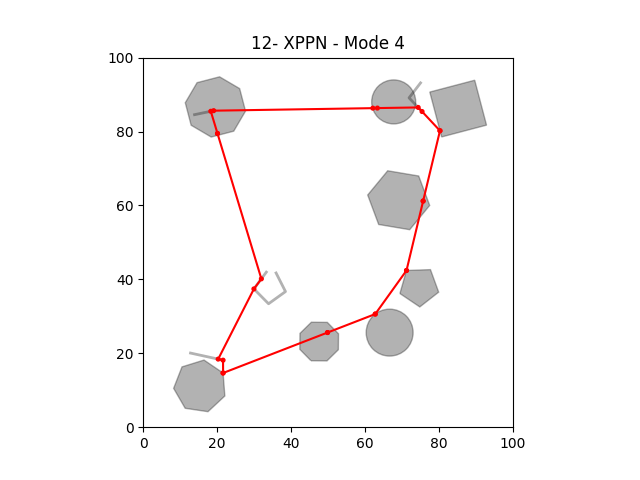
\includegraphics[width=0.8\linewidth]{example_xppn.png}
	\end{figure}
	\end{frame}

% Aqui va el ejemplo 2

	\begin{frame}{Example 2}
	    \begin{center}
			\animategraphics[controls, width = 0.7\linewidth]{3}{gif_xppn/}{100}{1}
		\end{center}
	\end{frame}
	
	\begin{frame}{Heuristic Algorithm}
	    \begin{algorithm}[H]
        %\SetKwInOut{Input}{Initial parameters}
        %\SetKwInOut{Output}{output}
        Let $\{\mathcal N_v:v\in V\}$ be the neighborhood set.
        Set $attempts=25$, $neigh\_size = 5$, $iter=10$.
        \begin{enumerate}
        \item Solve 
        \begin{mini*}|s|
         {}{\sum_{v\in V}\|x_v^i - \text{Med} \|}{}{}\label{weber}\tag{Weber}
        \addConstraint{\eqref{U-C}, \eqref{P-C}, \eqref{alpha-C}}{}{}
        \end{mini*}
        for $\{\mathcal N_v:v\in V\}$ to get $\bar{x}$.
        \item Consider the VNS approach with parameters $attempts$, $neigh\_size$ and $iter$ and points $\bar{x}$ to obtain the order of visit to the neighborhoods $\bar{z}$.
        \end{enumerate}
        
        \caption{Heuristic for solving XPPN.\label{alg:heuristic}}
        \end{algorithm}
	    
	\end{frame}
	
	\begin{frame}{Heuristic Algorithm: Clustering Phase}
        \begin{figure}[ht!]
        \begin{center}
         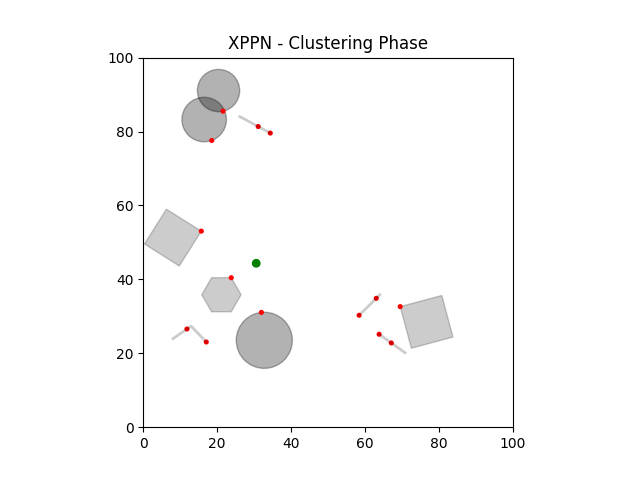
\includegraphics[width=0.7\linewidth]{XPPN - Clustering Phase}
        \end{center}
        \caption{Illustration of the first phase of the heuristic algorithm} \label{fig:heur-1}
        \end{figure}
	\end{frame}


	\begin{frame}{Heuristic Algorithm: VNS Phase}
        \begin{figure}[ht!]
        \begin{center}
         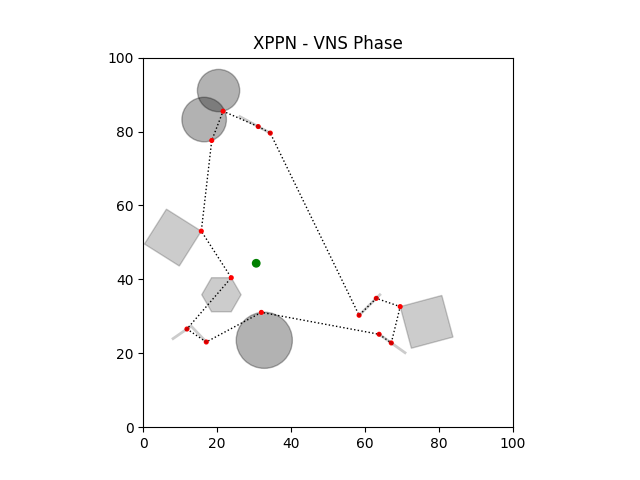
\includegraphics[width=0.7\linewidth]{XPPN - VNS Phase}
        \end{center}
        \caption{Application of the VNS phase to the example of Figure \ref{fig:heur-1} \label{fig:heur-2}}
        \end{figure}
	\end{frame}
	
	\begin{frame}{Strengthening results for the formulation: Preprocessing}
	\begin{small}
	\begin{block}{Remark 1}
		If the problem verifies that $f _v= 0$ for all $v\in V _{\mathcal C}$, then the entry and exit points $x_v^1$ and $x_v^2$ selected in each neighborhood are the same that the ones obtained by minimizing the distance between the neighborhoods.
	\end{block}
	
	    \begin{block}{Remark 2}
	        If $f_v\geq 1$ for some $v\in V_{\mathcal C}$, then, there exists an optimal solution verifying $x_v^1=x_v^2$.
	    \end{block}
	    
       	\begin{block}{Proposition 1}
            Given two neighborhoods $A$ and $B$, if $B\supset A$, then $B$ can be removed in the 						problem.
        \end{block}
	    \begin{block}{Proposition 2}
	        There exists always an optimal solution of the XPPN whose selected points are placed in the boundary of the neighborhoods.
	    \end{block}
	 \end{small}
	    
	 \end{frame}
	 
	 \begin{frame}{Strengthening results for the formulation: Preprocessing}
	    \begin{block}{Corollary 1}
	        Any point selected in an optimal solution of the XPPN when all the neighborhoods are circles is placed in some arc of one of the circumferences inside of the convex hull generated by the center of the circles.
	    \end{block}
	    
	    \begin{center}
         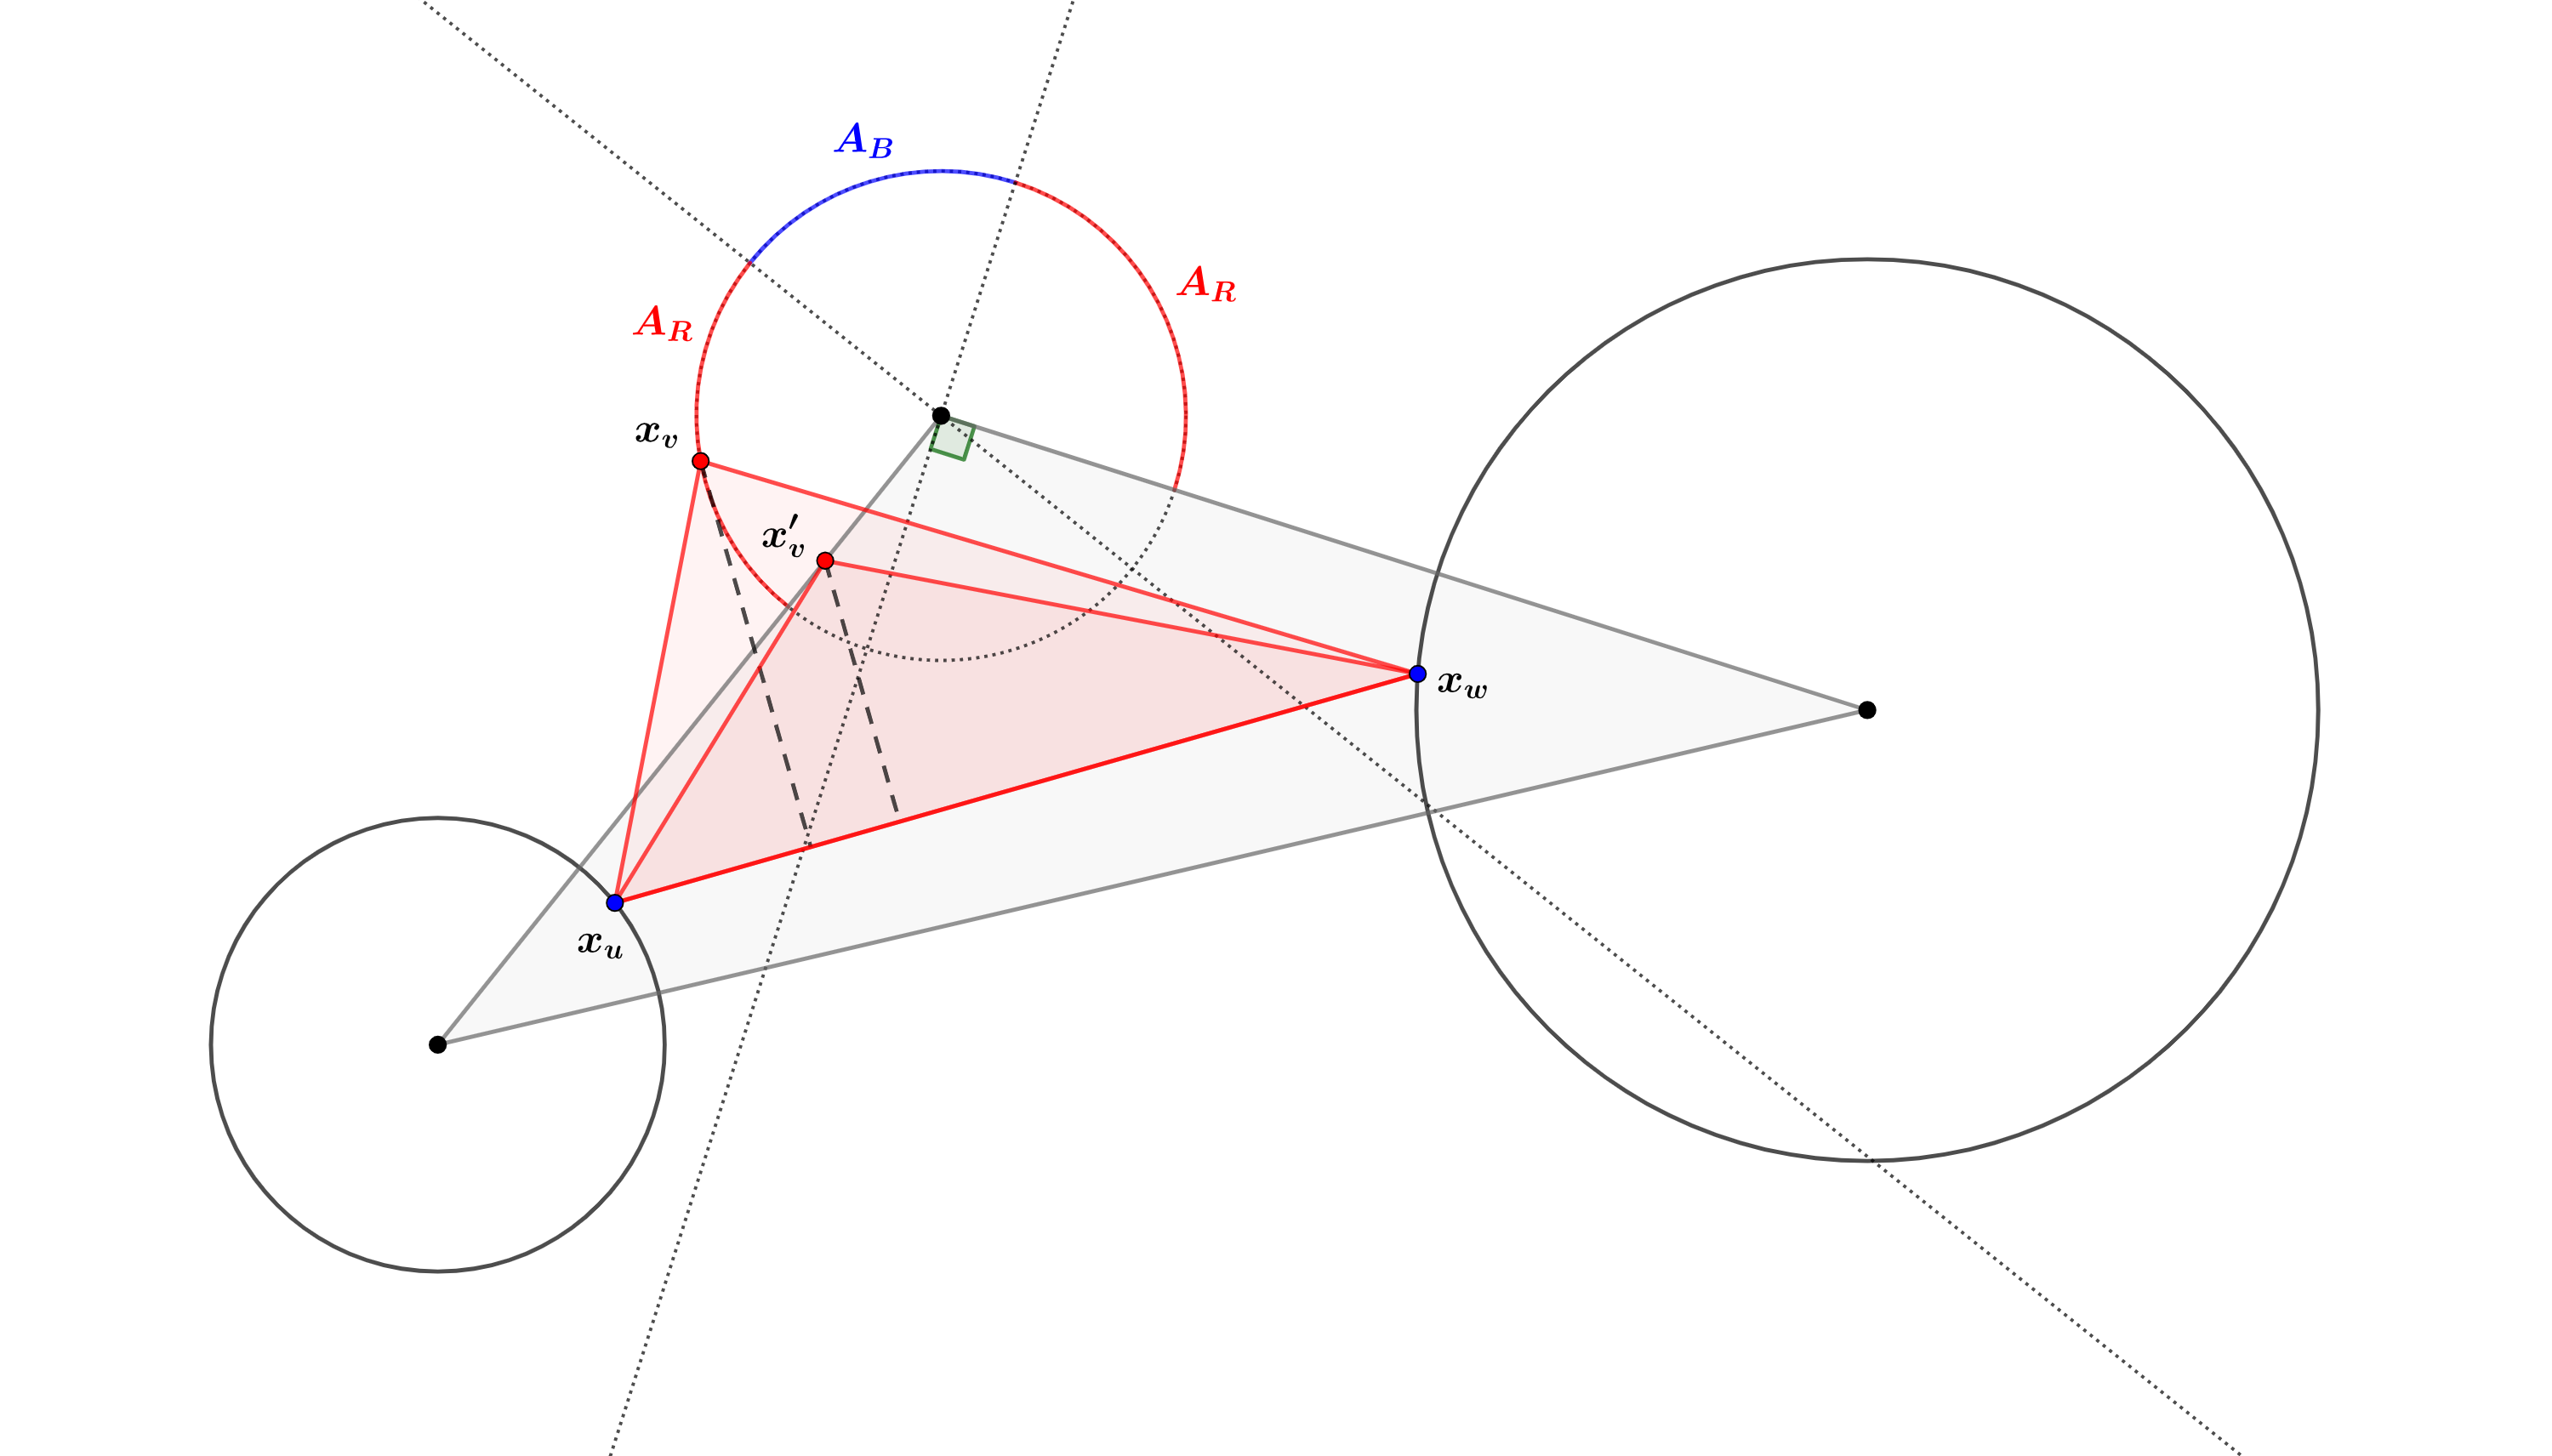
\includegraphics[width=0.45\linewidth]{XPPN-Corollary21a.png} \label{fig:corolario1}
         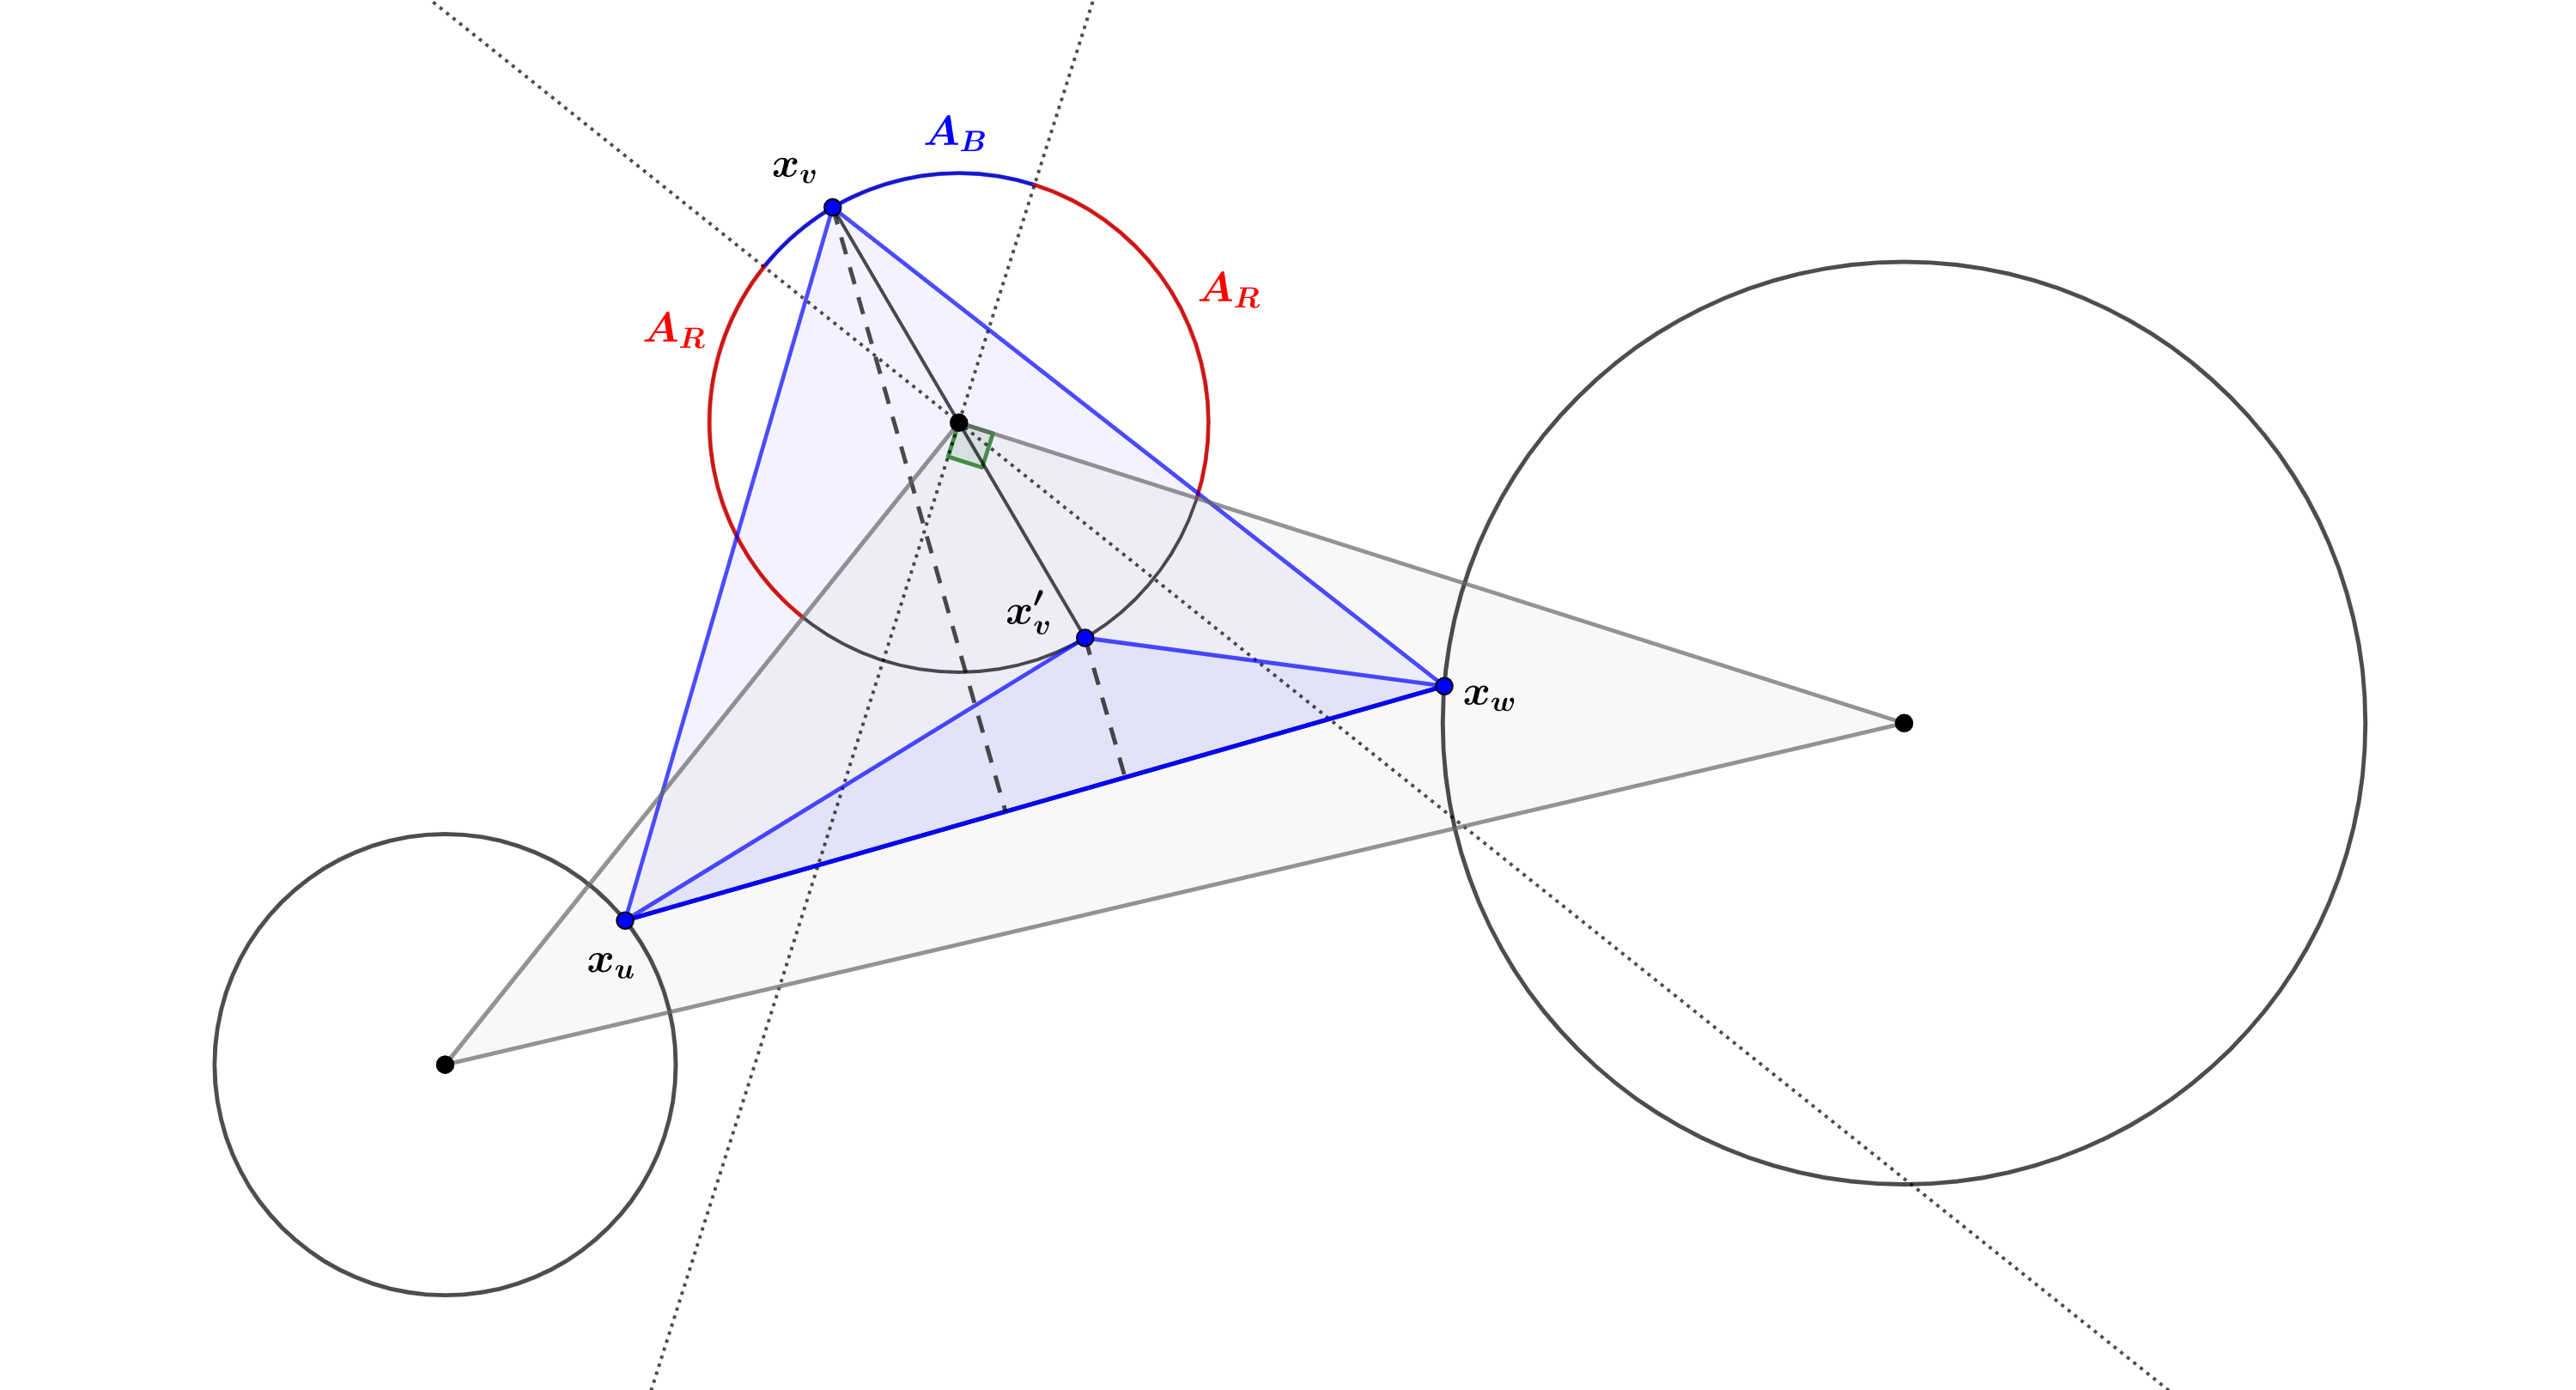
\includegraphics[width=0.45\linewidth]{XPPN-Corollary21b.png} \label{fig:corolario2}
        \end{center}
        
        


	\end{frame}

    \begin{frame}{Strengthening results for the formulation: Valid Inequalities}
        Adjusting $M_e$ (resp. $m_e$) that denotes an upper (resp. lower) bound of the distance between the sets joined by an edge $e \in E_{\text{out}}$.
        
        \begin{figure}
            \centering
            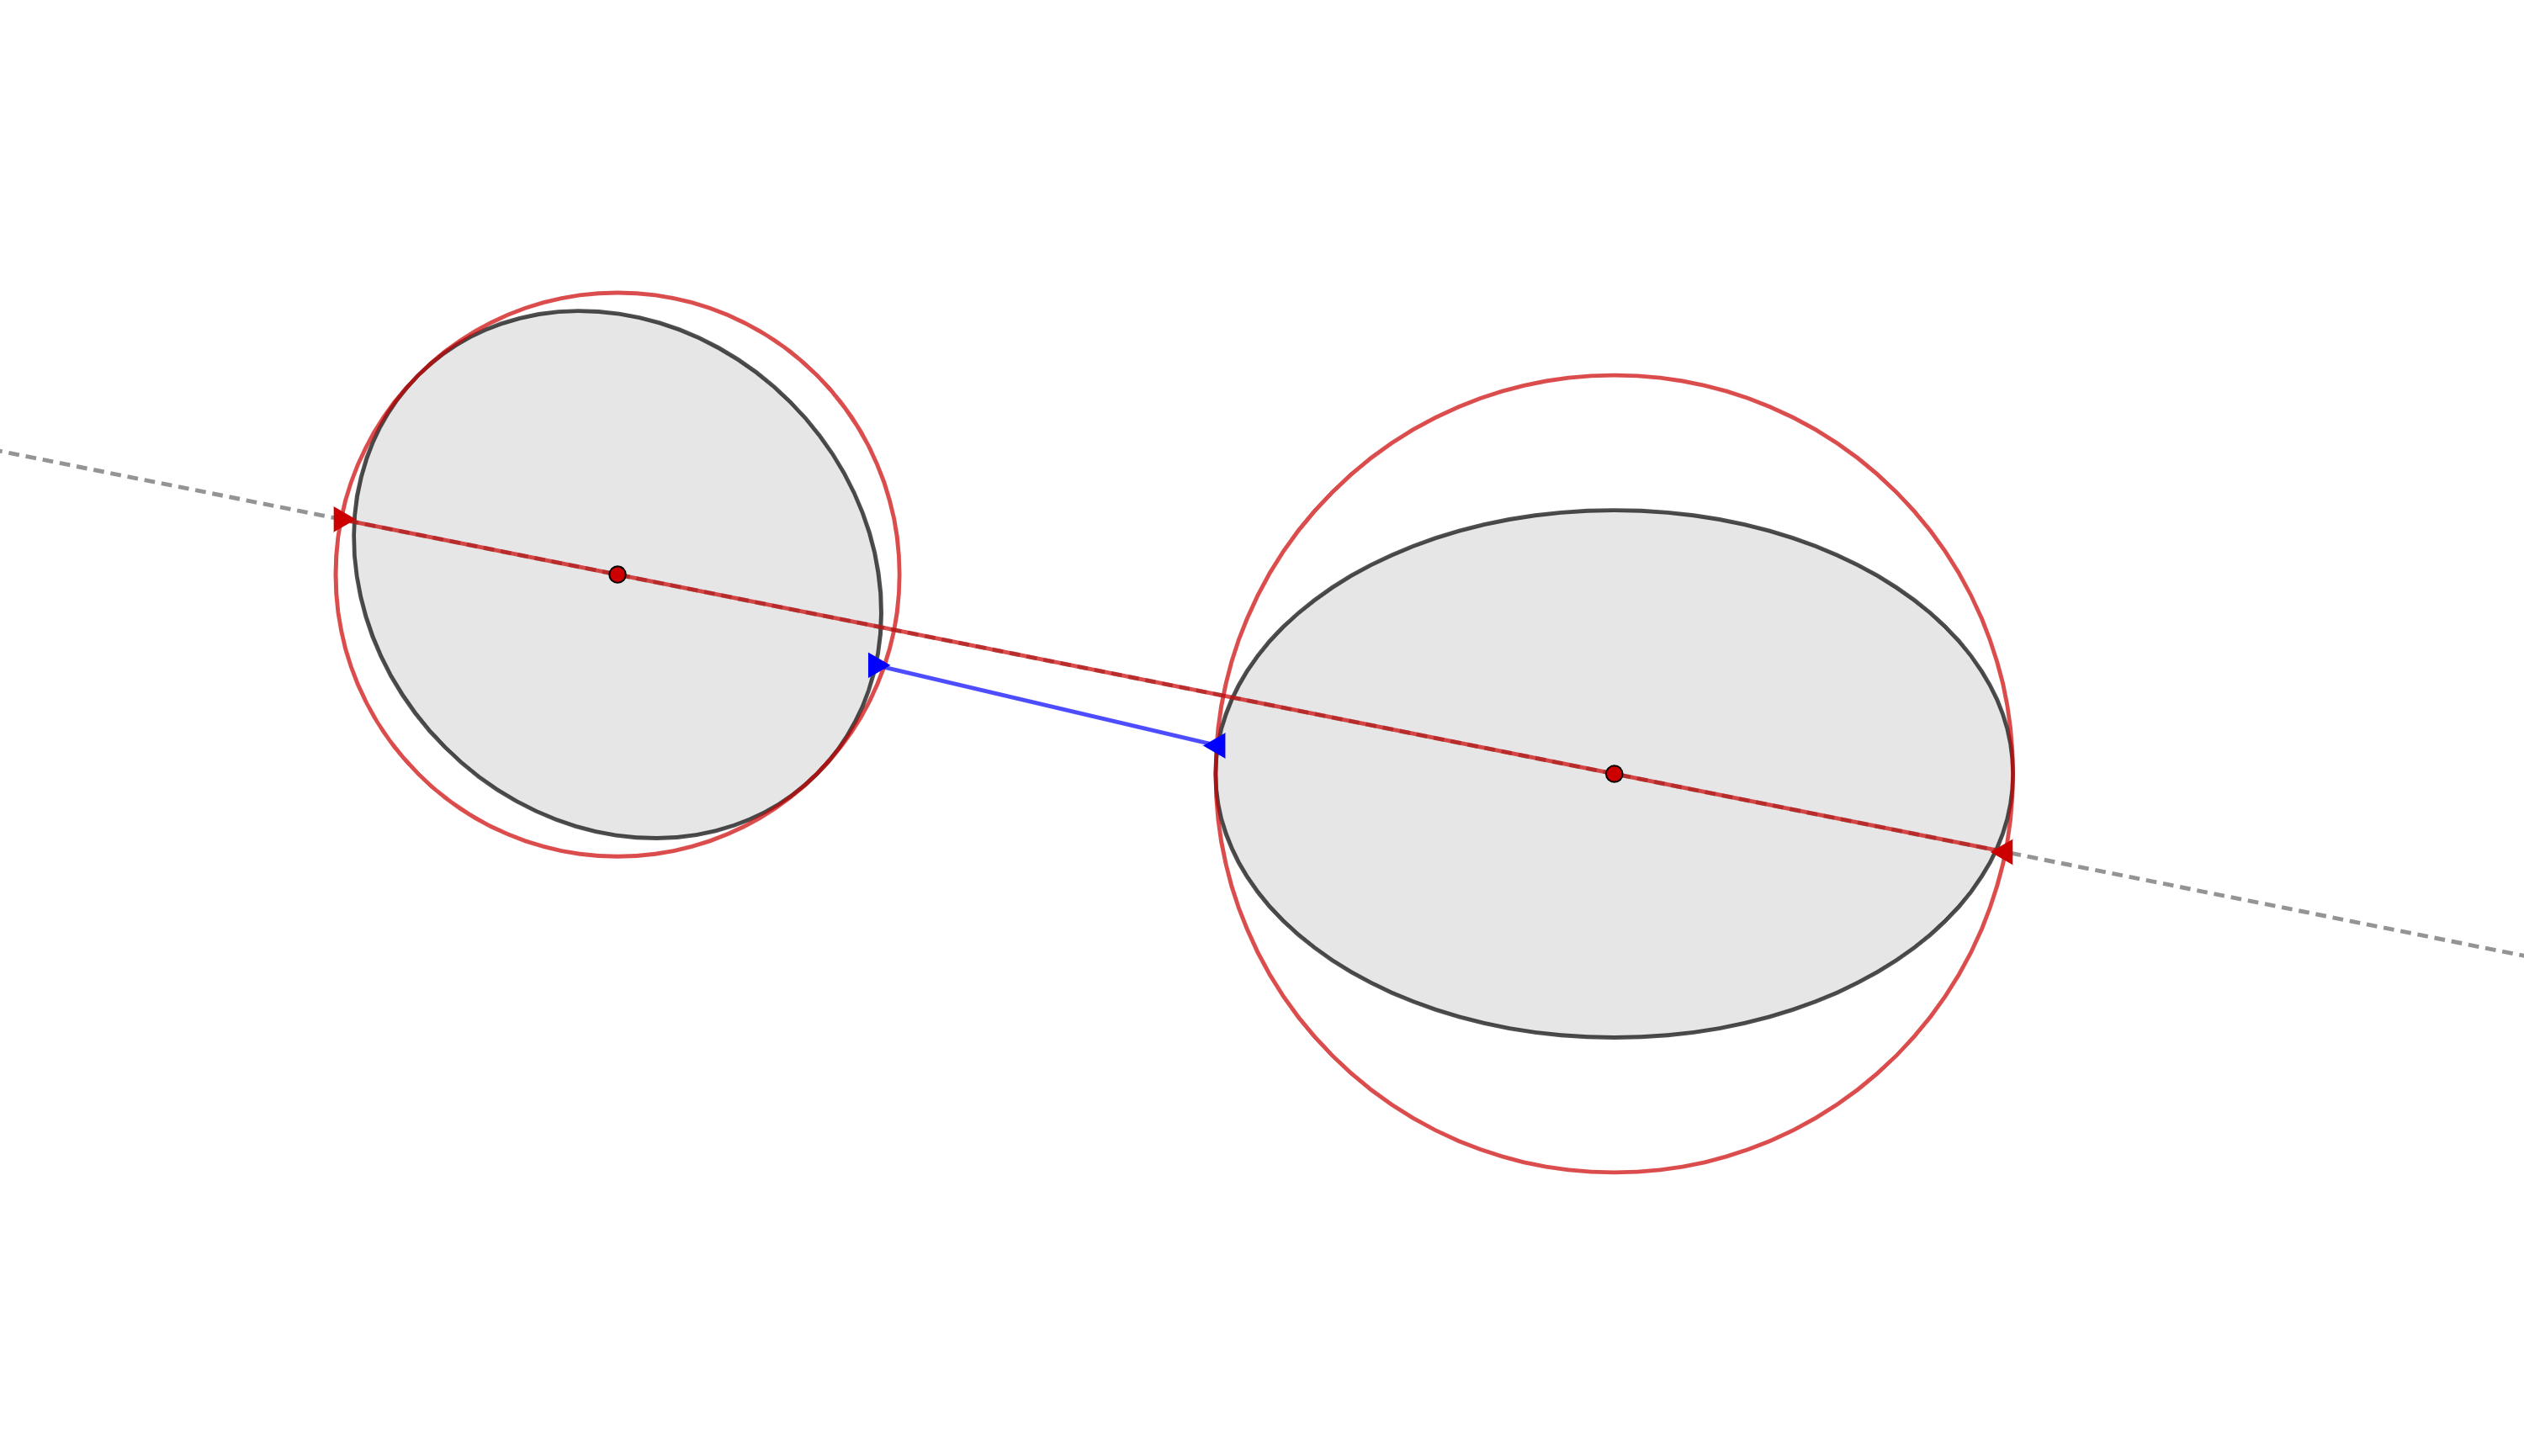
\includegraphics[width=0.7\linewidth]{bounds_ellip_ellip.png}
            \caption{Upper and lower bound when both sets are ellipsoids}
            \label{fig:boundsellipellip}
        \end{figure}
        
	\end{frame}
	
	\begin{frame}{Strengthening results for the formulation: Valid Inequalities}
        Adjusting $M_e$ (resp. $m_e$) that denotes an upper (resp. lower) bound of the distance between the sets joined by an edge $e \in E_{\text{out}}$.
        
        \begin{figure}
            \centering
            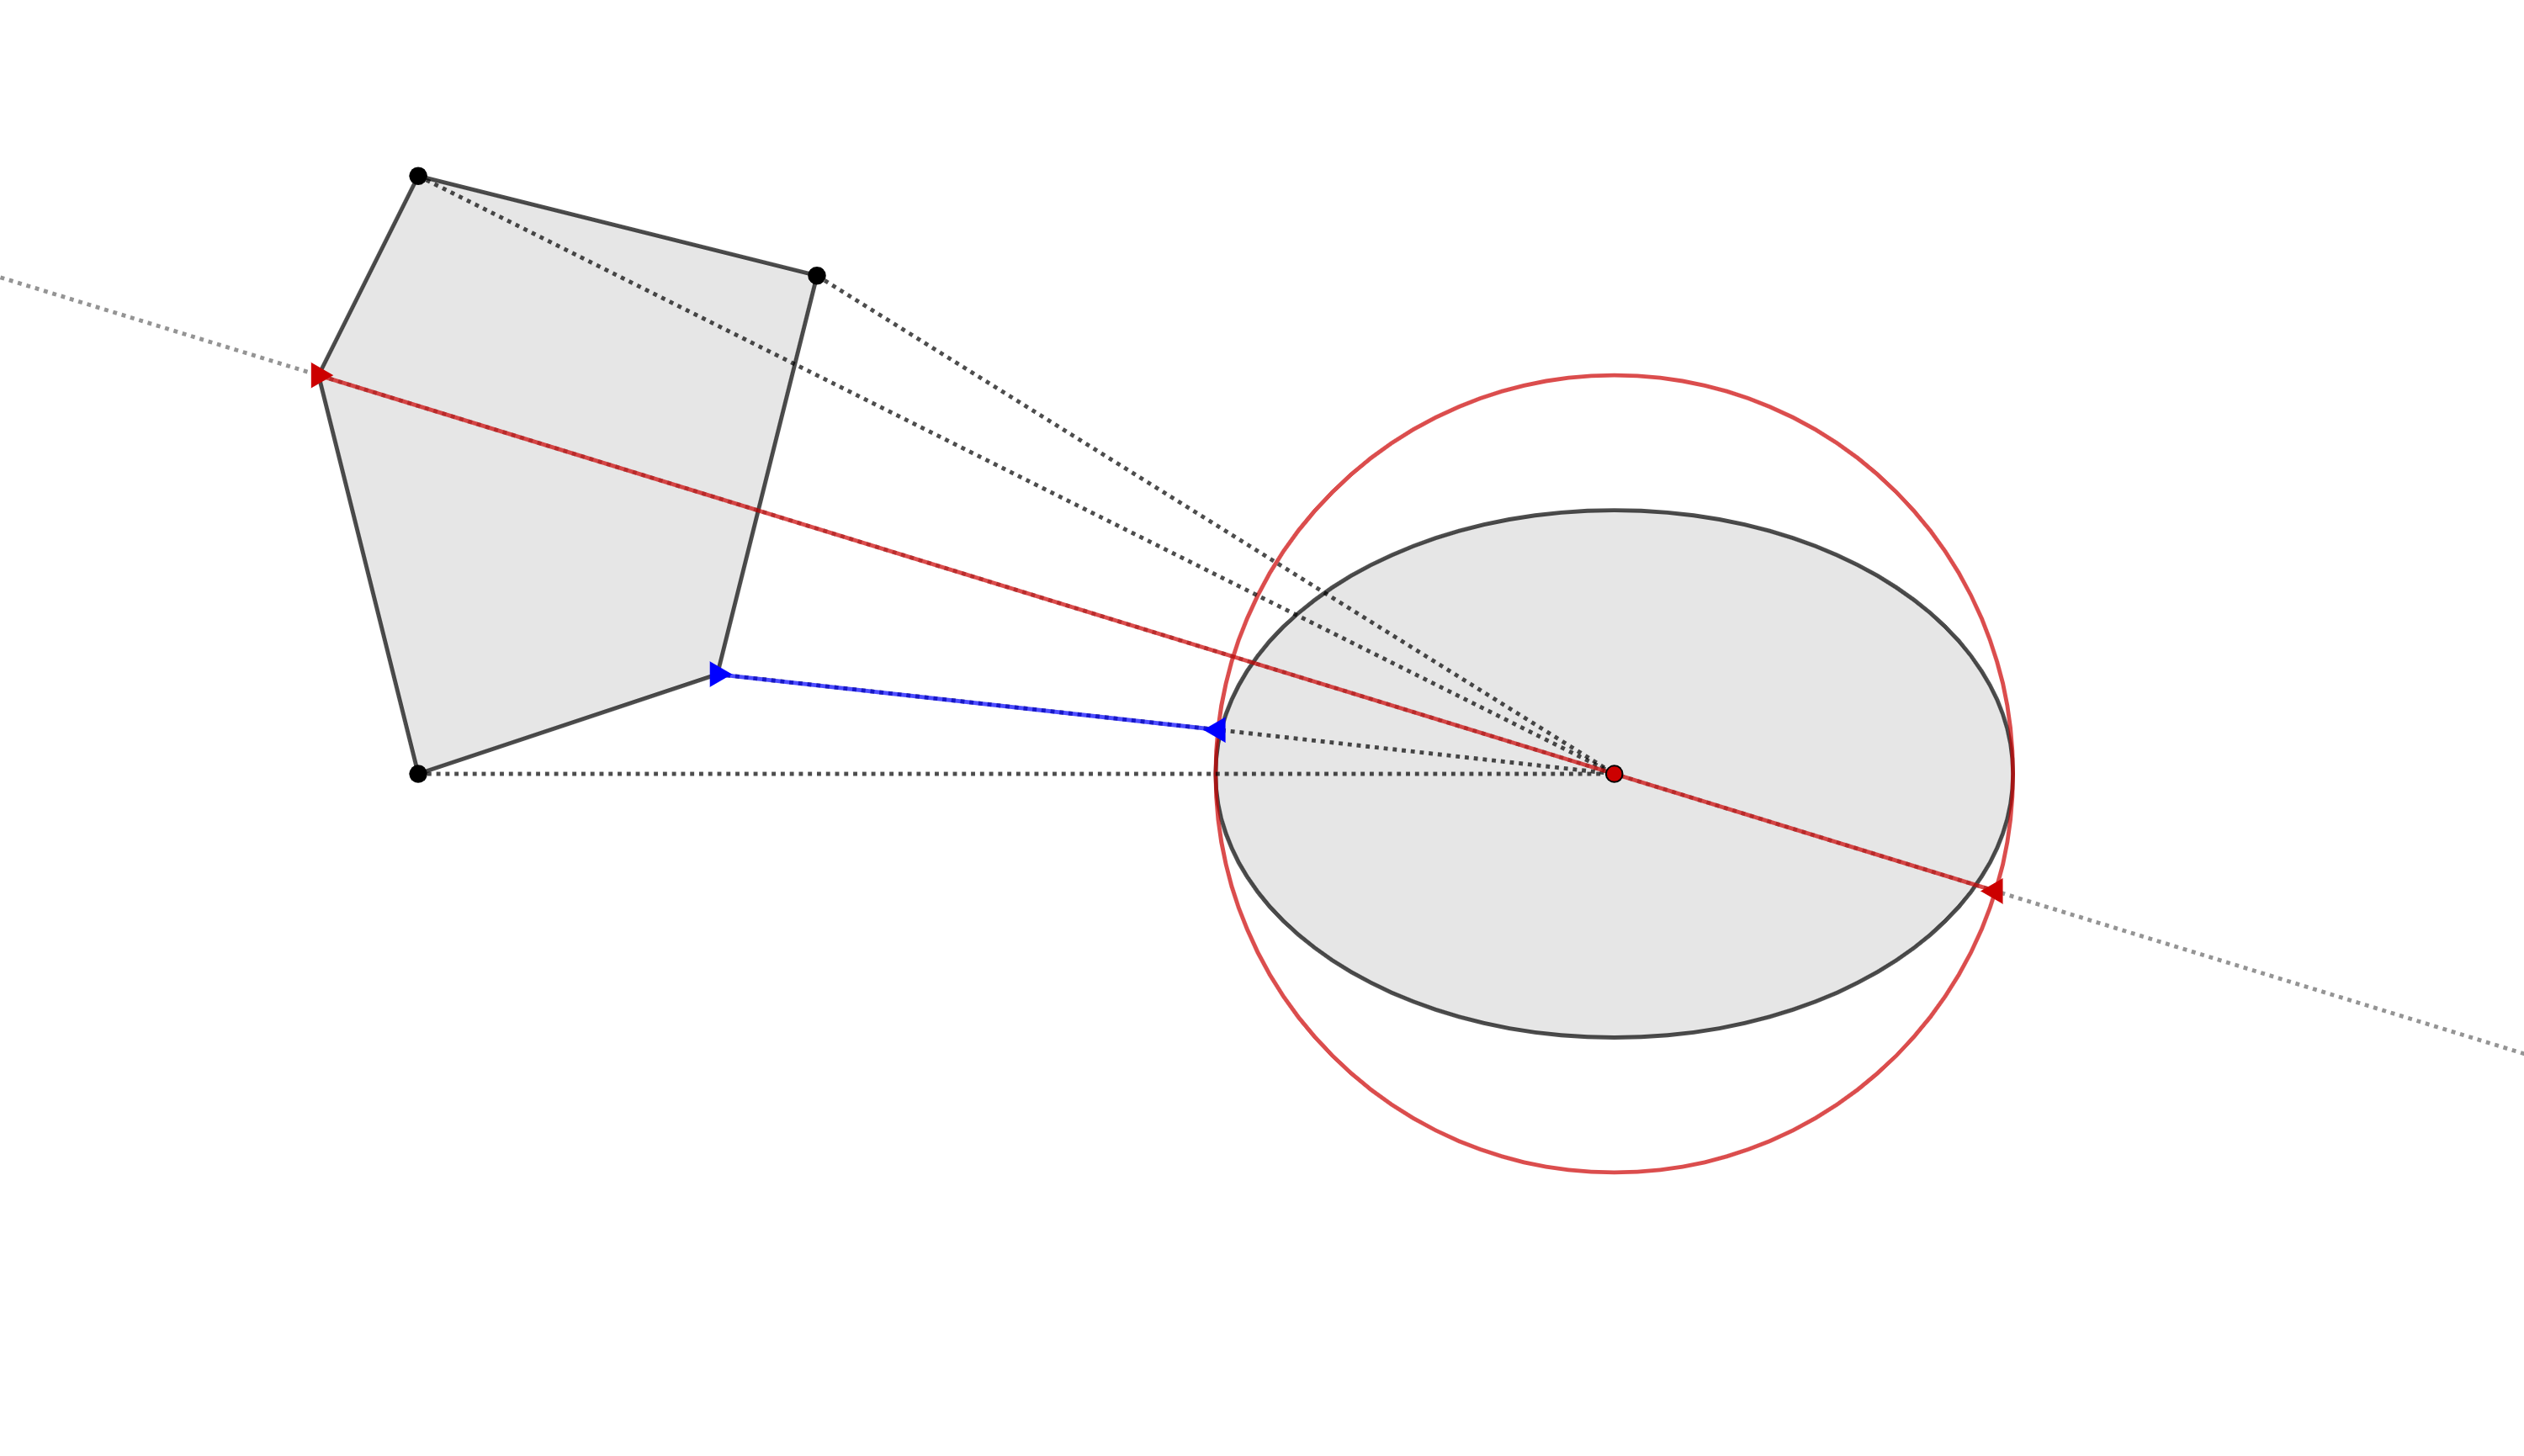
\includegraphics[width=0.7\linewidth]{bounds_ellip_polgon}
            \caption{Upper and lower bound when a set is a polygon and the other is an ellipsoid}
            \label{fig:boundsellipellip}
        \end{figure}
        
	\end{frame}
	
	\begin{frame}{Strengthening results for the formulation: Valid Inequalities}
        Adjusting $M_e$ (resp. $m_e$) that denotes an upper (resp. lower) bound of the distance between the sets joined by an edge $e \in E_{\text{out}}$.
        
        \begin{figure}
            \centering
            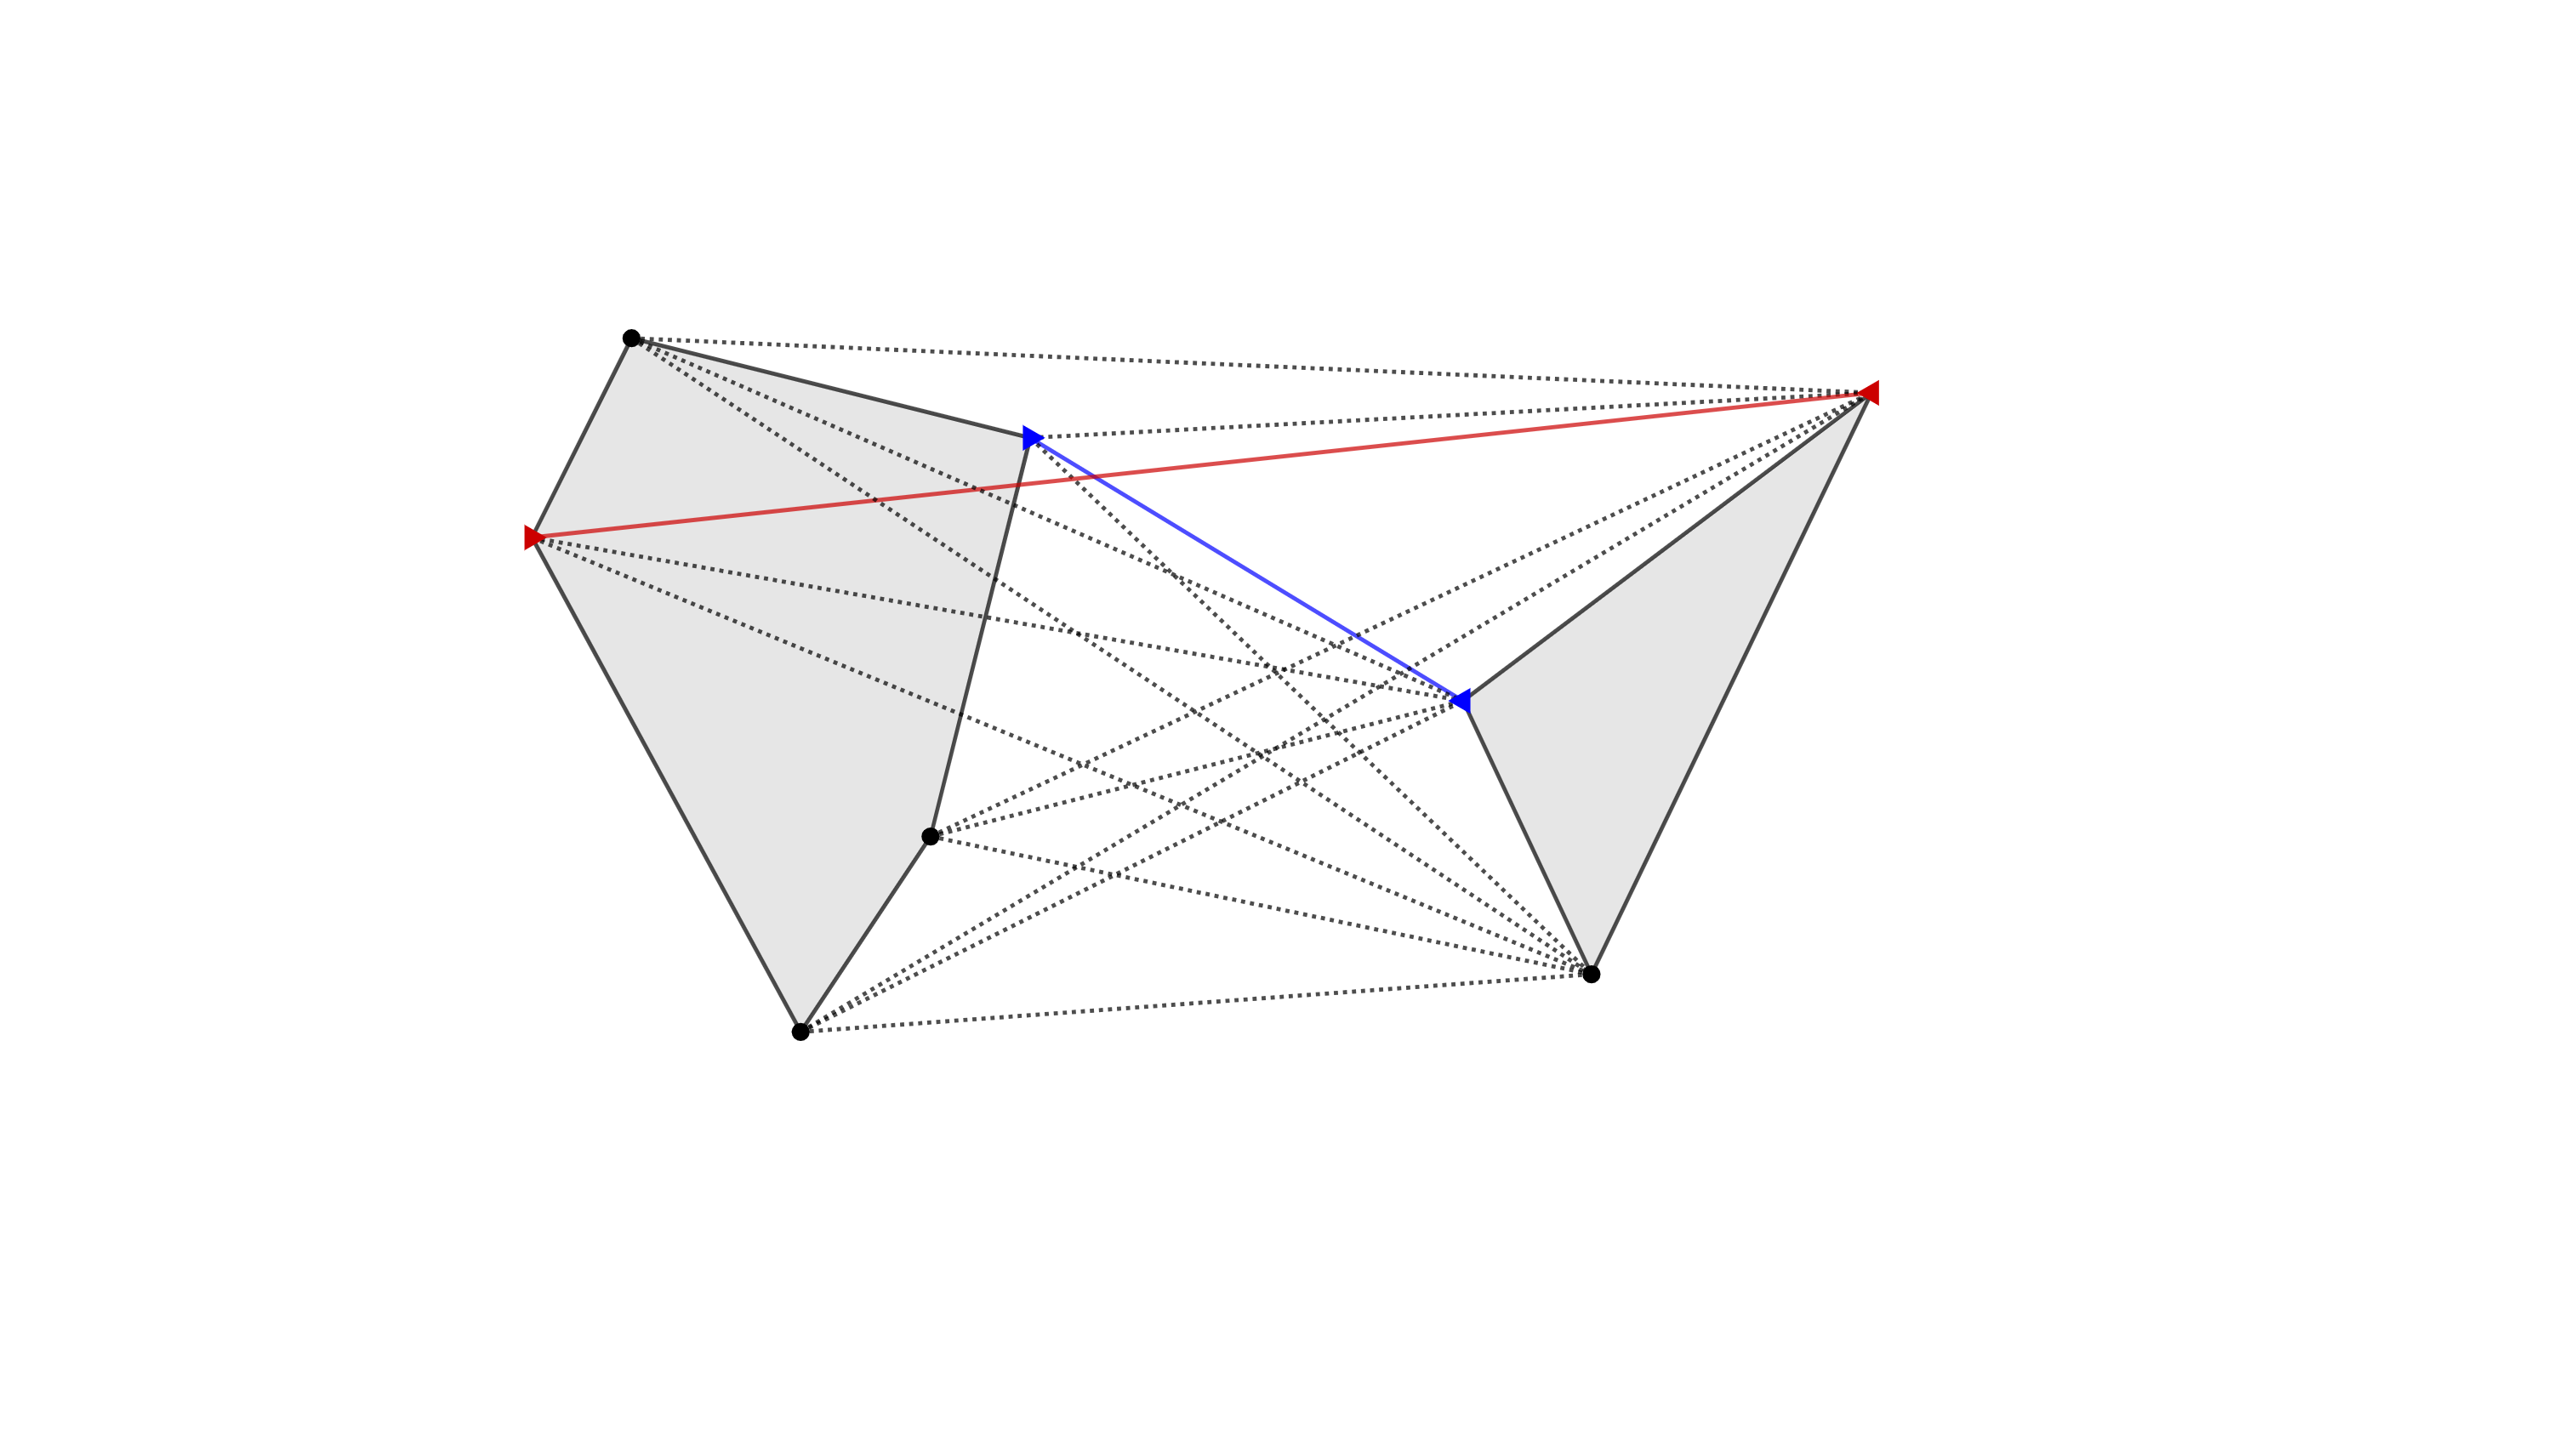
\includegraphics[width=0.7\linewidth]{bounds_polgon_polgon.png}
            \caption{Upper and lower bound when both sets are ellipsoids}
            \label{fig:boundsellipellip}
        \end{figure}
        
	\end{frame}
	
	\begin{frame}{Strengthening results for the formulation: Valid Inequalities}
        Adjusting $m_v$ that denotes the maximum distance between two points within a given neighborhood.
        
        \begin{figure}[h]
         \centering
         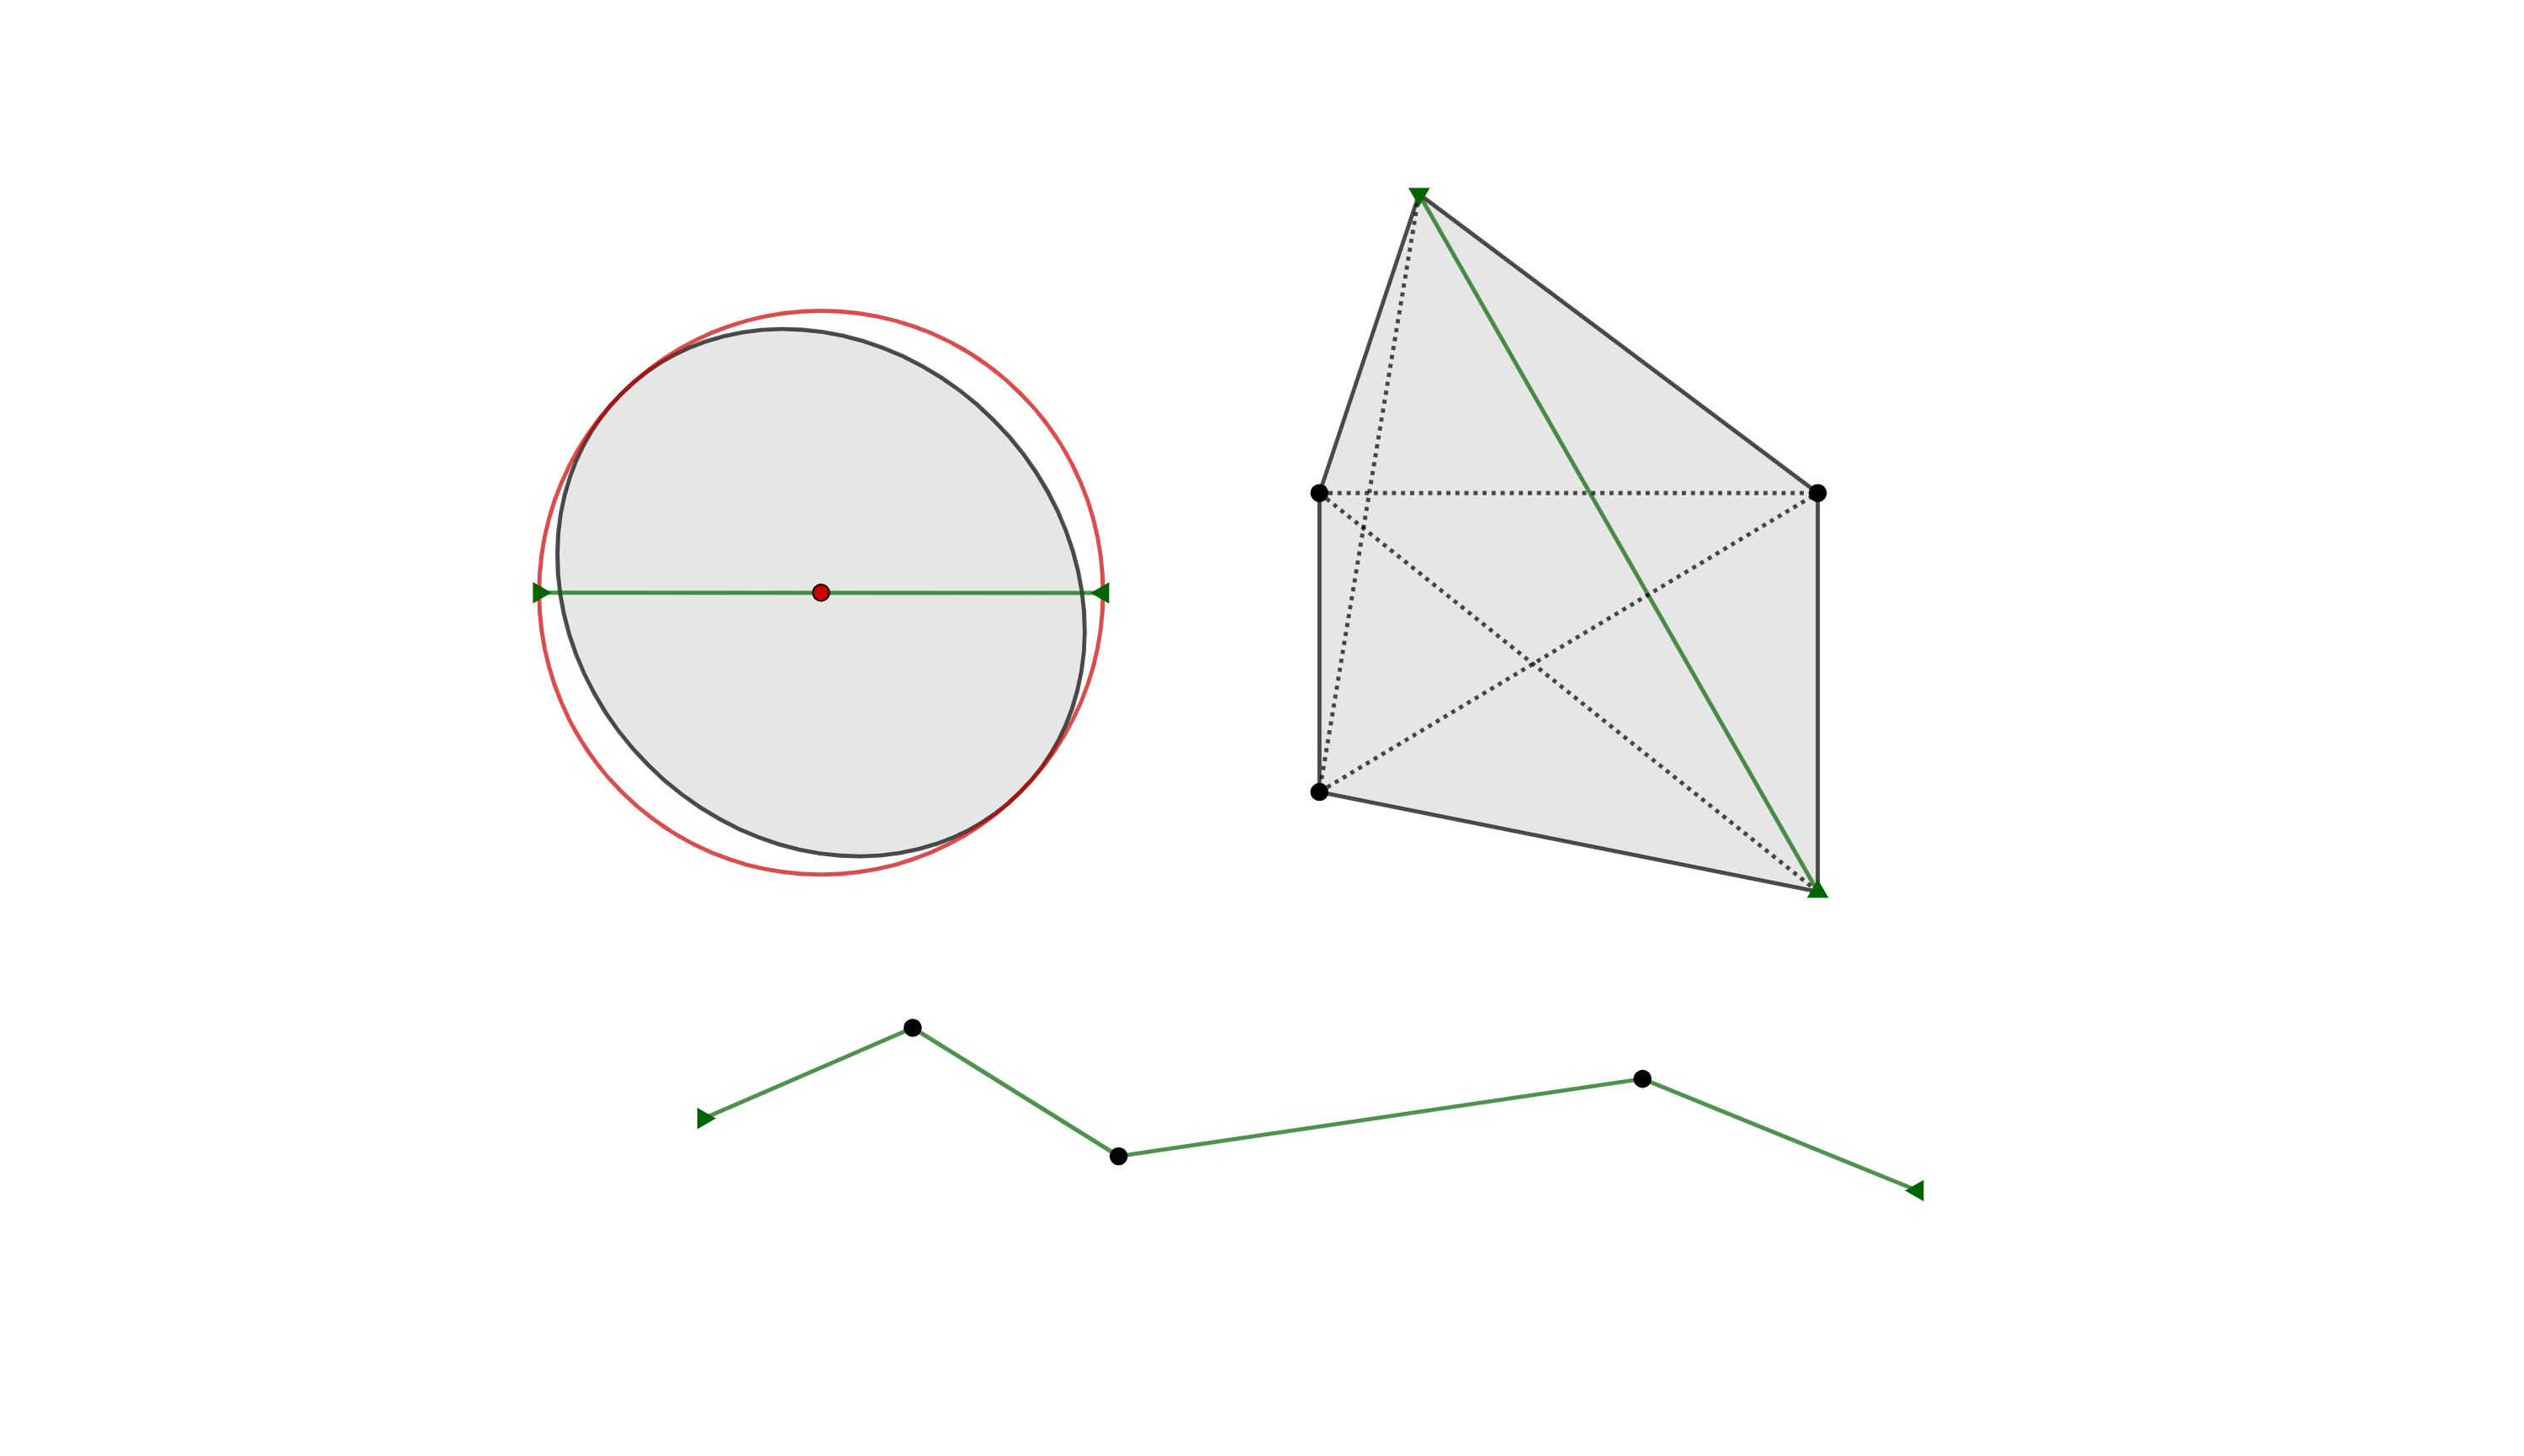
\includegraphics[width=0.7\linewidth]{bounds_inside}
         \caption{Upper bound on the maximal distance within a set}
         \label{fig:boundsinside}
        \end{figure}
            
	\end{frame}
	
	\begin{frame}{Benders decomposition}
	    \begin{footnotesize}
	    \begin{algorithm}[H]
            \SetKwInOut{Input}{Initialization}\SetKwInOut{Output}{output}
            
             \Input{Let $z^0\in \mathcal{T}_G$ be an initial  solution and $\varepsilon$ a given threshold value.\\
             Set $LB=0$, $UB=+\infty$, $\bar z=z^0$.}
            
             \While{$|UB-LB|>\varepsilon$}{
             \begin{enumerate}
            \item Solve 
            \begin{mini*}|s|
                {}{d(\bar z)=\sum_{e\in E_\text{out}} d_e \bar z_e + \sum_{v\in V} f_v d_v}{}{}\label{Pdz}\tag{Pd$\bar z$}
                \addConstraint{}{d_e\in\mathcal{D}_e,\,d_v\in\mathcal D_v.}{}{}
            \end{mini*}
            for $\overline z$ to get $d(\overline{z})$.
            \item Add the cut $ P \geq  d(\bar z) + \sum_{e:\bar z_e = 1}M_e(z_e - 1) + \sum_{e:\bar z_e = 0}m_e z_e$ to the current master problem.
            \item Obtain the optimal value $\bar{P}$ to the current master problem, and its associated solution $\bar z$.
            \item Update $LB=\max\{LB, \bar{P}\}$ and $UB=\min\{UB, \sum_{e\in E} d_e(\overline{z})\overline{z}_e +\sum_{v\in V} f_v d_v\}$
            \end{enumerate}
            }
            
            \caption{Decomposition Algorithm for solving XPPN.\label{alg:benders}}
            \end{algorithm}
        \end{footnotesize}
	\end{frame}
	
	\begin{frame}{Computational Experiments: Data Generation}
 	\begin{footnotesize}
	     Five instances with a number $|V|\in\{5,10,15, 20\}$ of neighborhoods. We have considered three different types of neighborhoods to be visited:
        \begin{itemize}
            \item Circles of radii $r$.
            \item Regular polygons of radii $r$ with a random number of vertices in the interval $[3, 10]$.
            \item Polygonal chains parameterized by its breakpoints that are at a distance of in $r$ from one another and some random percentage $\alpha\in [0, 1]$ of their length to be visited.
        \end{itemize}
	    
	    The centers or breakpoints of these elements have been generated uniformly in the square [0, 100]. On the one hand, we have studied four different scenarios to generate the radii to define the elements:
        \begin{itemize}
        	\item \textbf{Small size Neighborhoods} $(r=1)$: Radii randomly generated in $[0, 5]$.
        	\item \textbf{Small-Medium Neighborhoods} $(r=2)$: Radii randomly generated in $[5, 10]$.
        	\item \textbf{Medium-Large size Neighborhoods} $(r=3)$: Radii randomly generated in $[10, 15]$.
        	\item \textbf{Large size Neighborhoods} $(r=4)$: Radii randomly generated in $[15, 20]$.
        \end{itemize}
    \end{footnotesize}
    \end{frame}
    
    \begin{frame}
        We have also considered four modes depending on the nature of the neighborhoods:

        \begin{itemize}
        	\item Mode 1: All neighborhoods are circles.
        	\item Mode 2: All neighborhoods are regular polygons.
        	\item Mode 3: All neighborhoods are polygonal chains.
        	\item Mode 4: Mixture of the three previously  considered neighborhoods.
        \end{itemize}
        
        \bigskip
        All the formulations were coded in Python 3.7, and solved using Gurobi 9.0 in a Intel(R) Xeon(R) E-2146G CPU @ 3.50 GHz and 64GB of RAM. A time limit of 2 hours was set in all the experiments.
        
            % \end{scriptsize}
	\end{frame}
	
	\begin{frame}{Comparing time and non-time dependent formulations}
    \begin{itemize}
        \item Easiest configuration corresponding to neighborhoods given by circles of small radius (Mode 1 and $r=1$).
        \item Size $n= 10$ neighborhoods: instances solved to optimality on average in 1800 sec.
        \item Size $n= 12$ neighborhoods: instances not solved to optimality within 7200 sec. 
        \begin{itemize}
            \item 20 \% does not find a feasible solution
            \item The average gap of the rest was above 80 \%.
        \end{itemize}
    \end{itemize}
    
    \bigskip
    Conclusion: We have restricted ourselves to the comparisons of the non-time dependent formulations presented
	\end{frame}
	
	\begin{frame}{\large Assessing the difficulty of the problems depending on the $\alpha$ parameter}
	    \begin{itemize}
	        \item Batch of 5 instances involving only polygonal chains that are fixed.
	        \item Varying only the $\alpha$ parameter in $\{0, 0.1,0.2,\ldots,0.9,1\}$.
	    \end{itemize}

        \begin{figure}
         \centering
         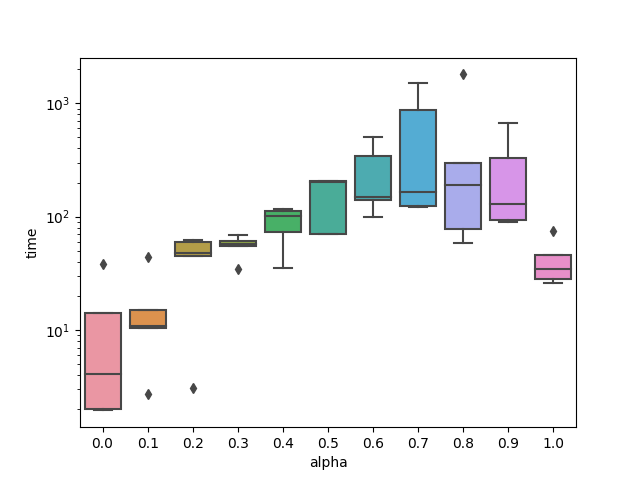
\includegraphics[width=0.6\linewidth]{time_alpha.png}
         \caption{Comparison of the times of the MTZ formulation varying the $\alpha$ parameter}
         \label{fig:dibujo_alpha}
        \end{figure}

	\end{frame}
	
	\begin{frame}{Initializing the solver with a heuristic solution}
	    \begin{itemize}
	        \item Comparing the MTZ formulation with and without initial solution provided by our proposed heuristic.
	        \item Sizes 5, 10 and 15.
	        \item Sizes 5 and 10 were solved to optimality.
	        \item For size 15:
	    \end{itemize}
	    \begin{figure}[h!]
         \centering
         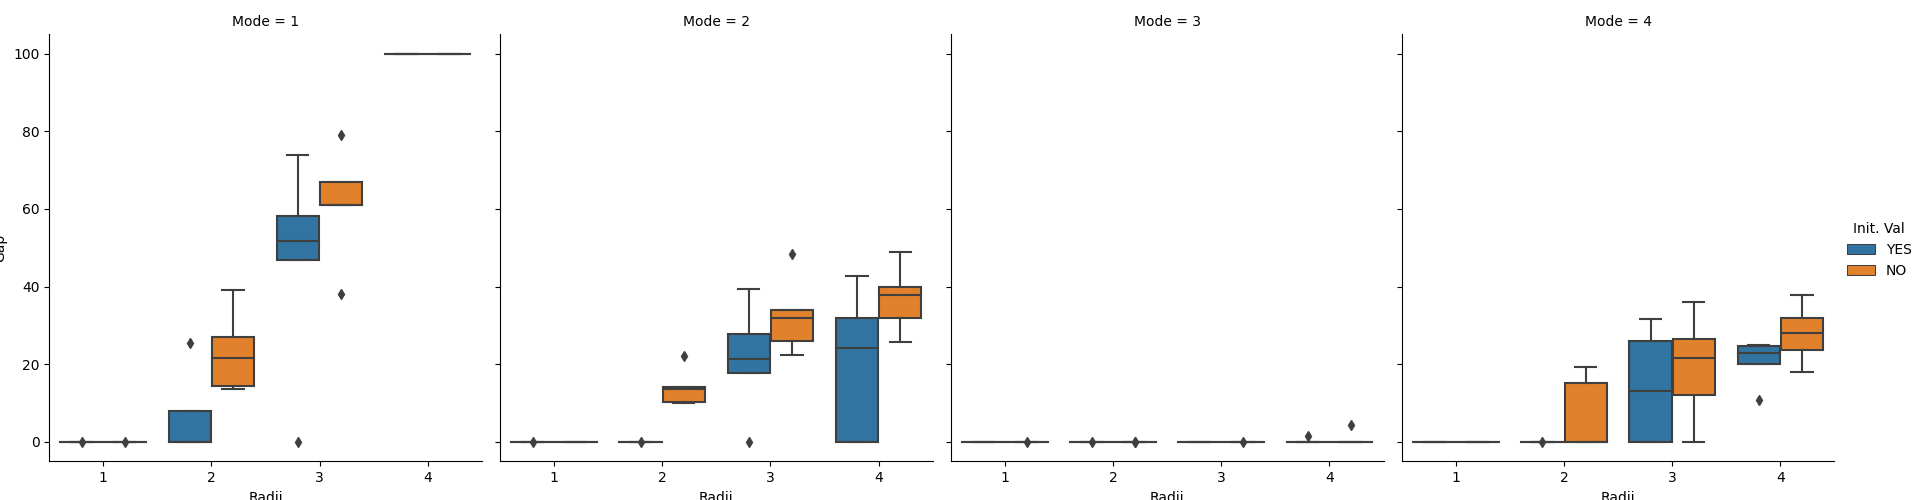
\includegraphics[width=1\linewidth]{final_gap_MTZs.png}
         \caption{Comparison of the final gap between MTZ formulation with and without initial solution after 7200 seconds for instances with 15 neighborhoods}
         \label{fig:final_gap}
        \end{figure}
	\end{frame}
	
	\begin{frame}{Comparing Benders cuts with the MTZ formulation}
	    \begin{itemize}
	        \item Comparing the decomposition algorithm described before with the MTZ formulation without initialization for size 10.
	    \end{itemize}
	    \begin{table}[h!]
            \centering
            \begin{threeparttable}
            \resizebox{\textwidth}{!}{%
            \begin{tabular}{|c|c|c|c|c|c|c|c|}
            \hline
            \textbf{Size} & \textbf{Radii} & \textbf{Mode} & \textbf{Final Gap (Benders)} & \textbf{Time (Benders)} & \textbf{\#Cuts} & \textbf{Final Gap (MTZ)} & \textbf{Time (MTZ)} \\ \hline
            10 & 1 & 1 & 0.0 & 15.72 & 19.0 & 0.0 & 1.93 \\ \hline
            10 & 1 & 2 & 0.0 & 23.64 & 55.4 & 0.0 & 0.75 \\ \hline
            10 & 1 & 3 & 0.0 & 13.22 & 25.8 & 0.0 & 0.72 \\ \hline
            10 & 1 & 4 & 0.0 & 33.96 & 29.8 & 0.0 & 1.52 \\ \hline
            10 & 2 & 1 & 76.1 & 6430.08 & 1209.0 & 0.0 & 38.83 \\ \hline
            10 & 2 & 2 & 56.14 & 4777.58 & 1009.6 & 0.0 & 14.14 \\ \hline
            10 & 2 & 3 & 0.0 & 1766.06 & 380.6 & 0.0 & 2.23 \\ \hline
            10 & 2 & 4 & 10.57 & 5993.57 & 804.6 & 0.0 & 2.52 \\ \hline
            10 & 3 & 1 & 96.21 & 7208.56 & 1481.2 & 0.0 & 487.94 \\ \hline
            10 & 3 & 2 & 92.16 & 7203.99 & 1352.2 & 0.0 & 35.81 \\ \hline
            10 & 3 & 3 & 9.29 & 5832.51 & 520.4 & 0.0 & 13.28 \\ \hline
            10 & 3 & 4 & 84.41 & 7214.86 & 921.8 & 0.0 & 133.81 \\ \hline
            10 & 4 & 1 & 98.79 & 7205.35 & 2283.0 & 19.28 & 3513.38 \\ \hline
            10 & 4 & 2 & 95.53 & 7207.51 & 1343.4 & 0.0 & 238.98 \\ \hline
            10 & 4 & 3 & 19.55 & 7220.14 & 499.0 & 0.0 & 20.25 \\ \hline
            10 & 4 & 4 & 82.69 & 7211.46 & 789.8 & 0.0 & 1142.17 \\ \hline
            \end{tabular}%
            }
            \caption{Computational comparison between MTZ formulation and Benders algorithm for problems with up to 10 neighborhoods}
            \label{tab:benders}
            \end{threeparttable}
            \end{table}
	\end{frame}
	
	\begin{frame}
	    \begin{figure}[h!]
         \centering
         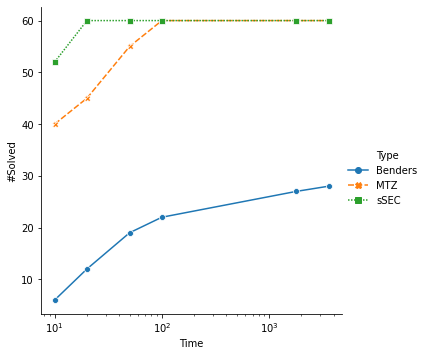
\includegraphics[width=0.6\linewidth]{instances_solved_benders.png}
         \caption{Performance profile: Time vs \#Solved }
         \label{fig:instances_solved_benders}
        \end{figure}
    \end{frame}
    
    \begin{frame}{Comparing MTZ, SEC and sSEC with initialization}
         \begin{figure}[h!]
          \centering
          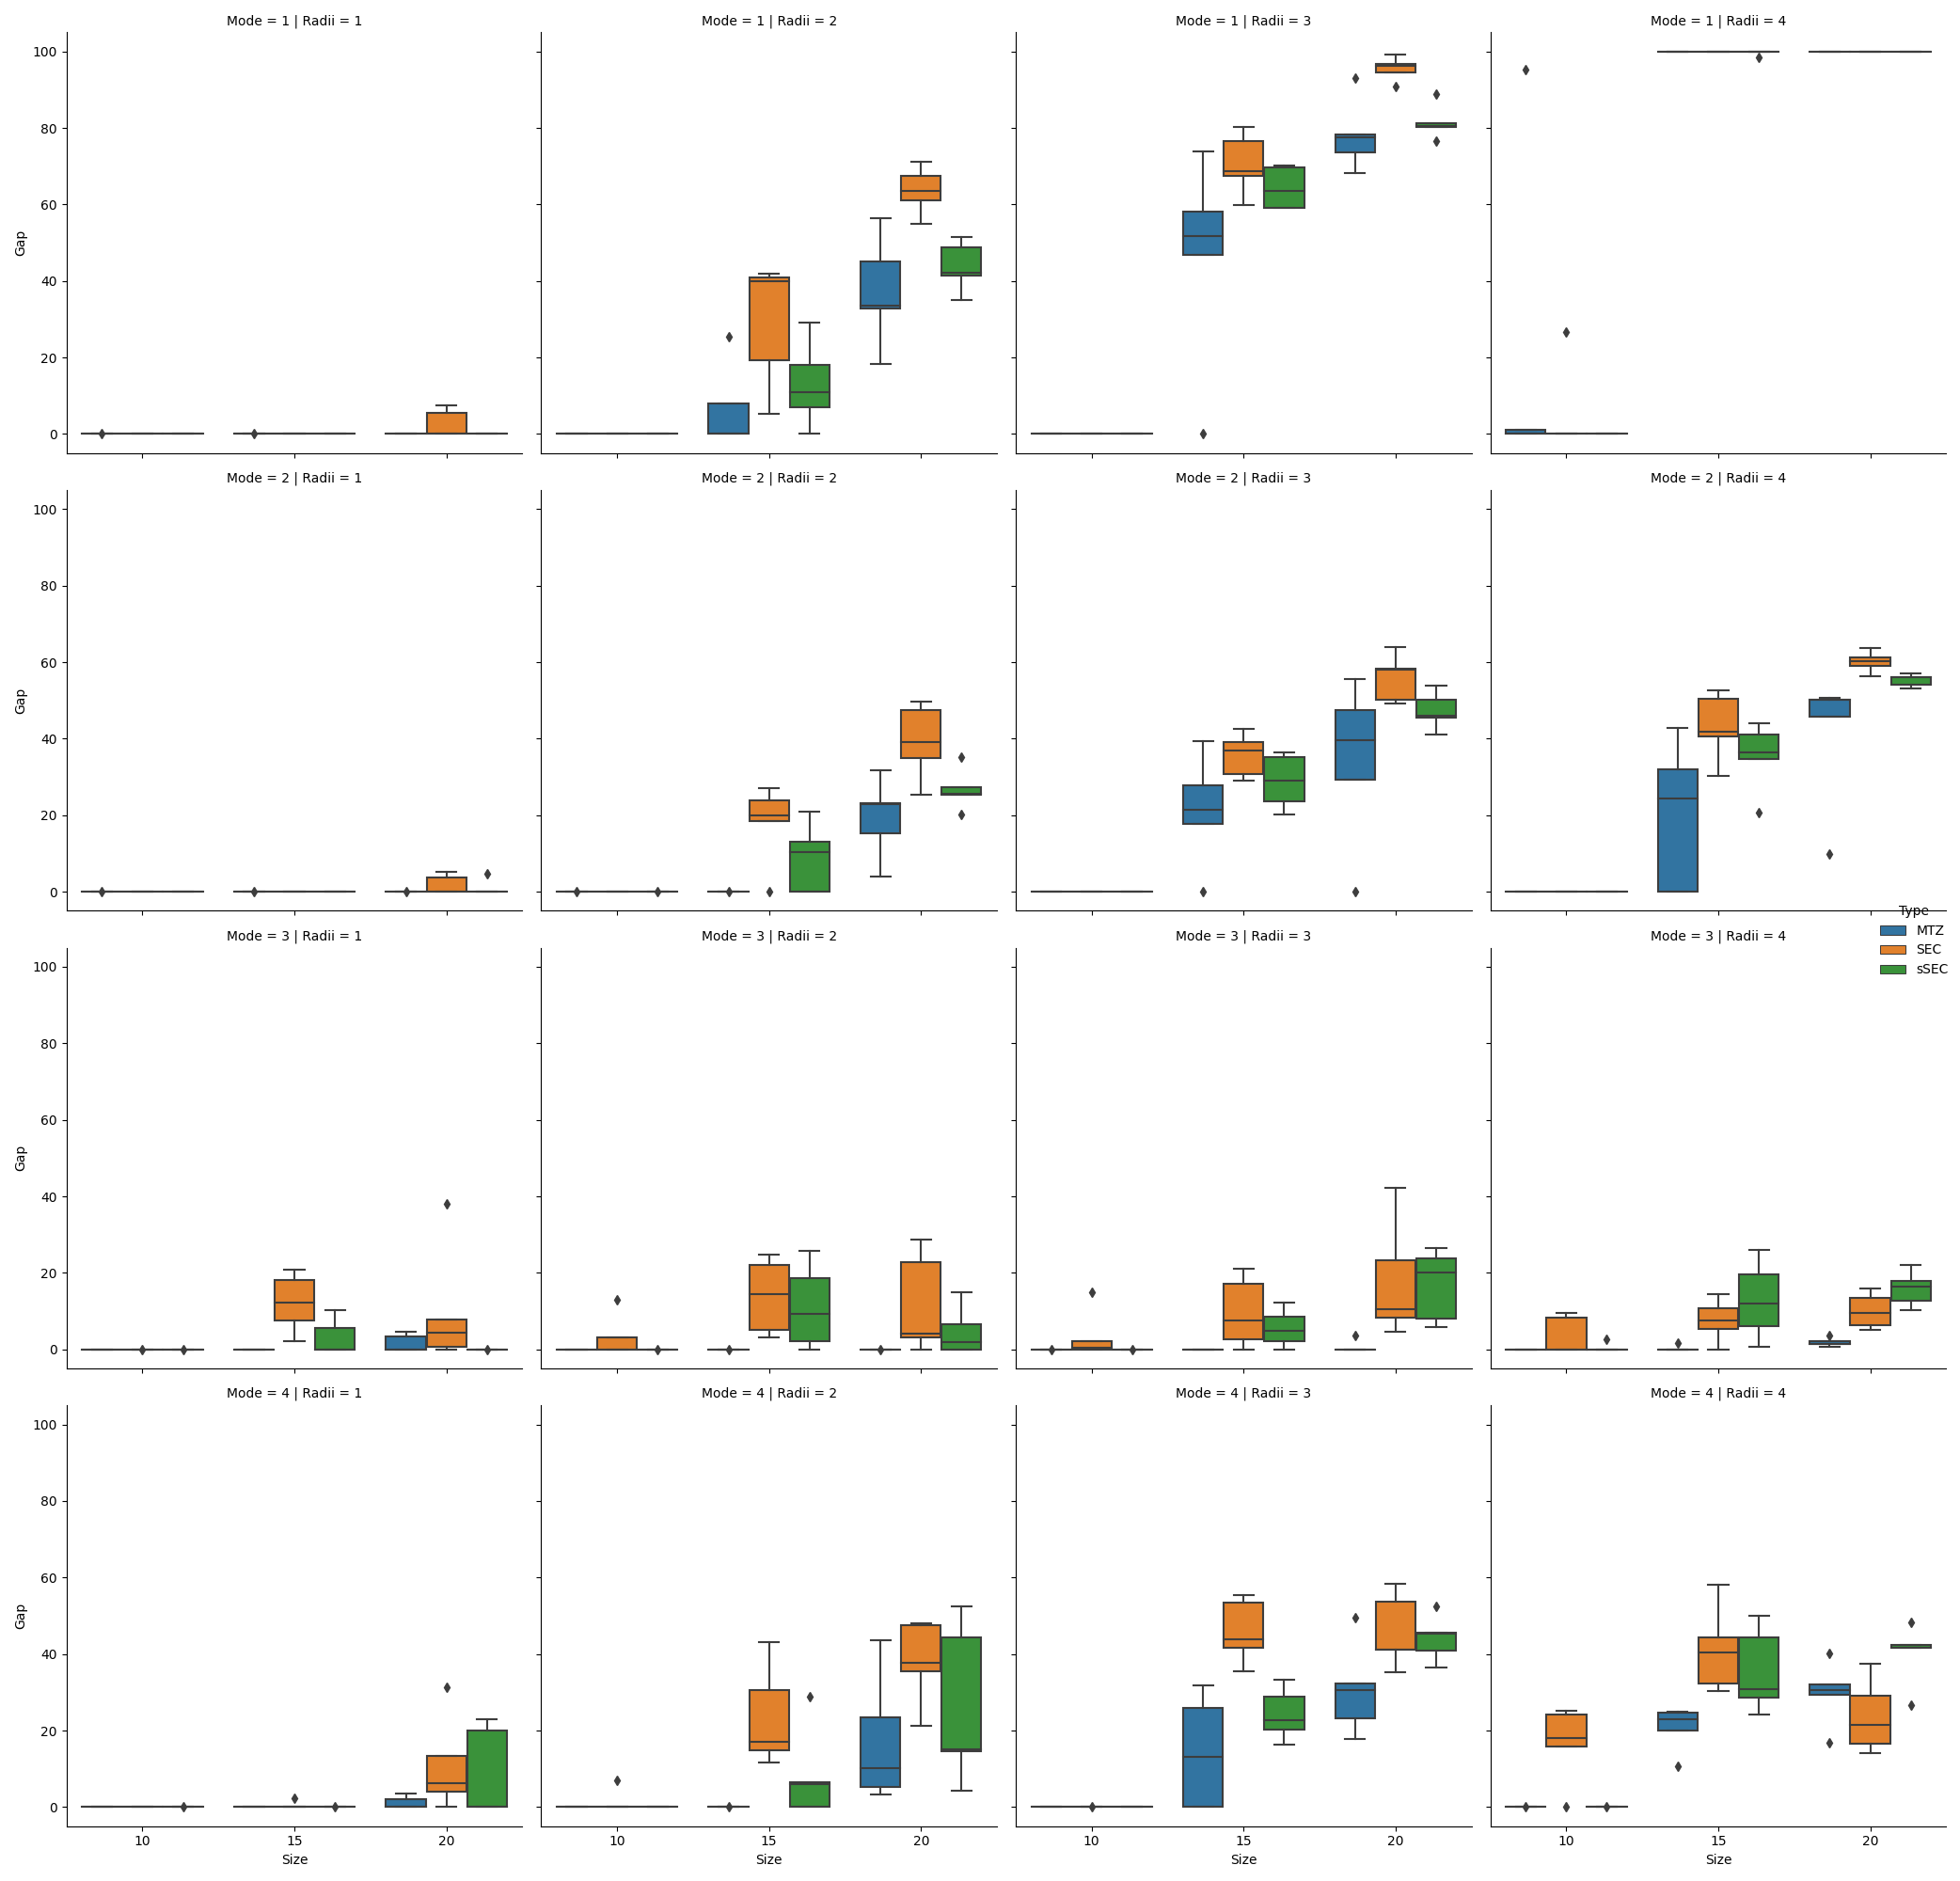
\includegraphics[width=0.7\linewidth]{final_gap.png}
          \caption{Final gap after 7200 seconds}
          \label{fig:final_gap2}
         \end{figure}
    \end{frame}
    
    \begin{frame}{Comparing MTZ, SEC and sSEC with initialization}
         \begin{figure}[h!]
          \centering
          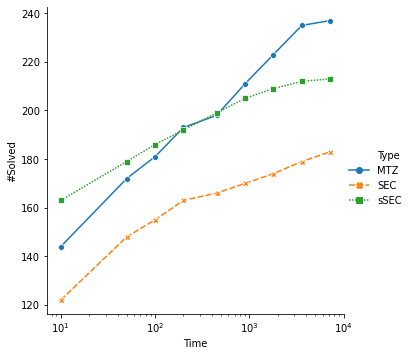
\includegraphics[width=0.5\linewidth]{instances_solved.png}
          \caption{Performance profile: Time vs \#Solved}
          \label{fig:profile}
         \end{figure}
    \end{frame}
	
	\section{Coordinated Models: The MDRPG}
	\begin{frame}{Contents}
	    \begin{itemize}
		    \item Problem Description
		    \item Formulations
		    \begin{itemize}
		        \item The AMDRPG.
		        \item The PMDRPG.
		        \item The NMDRPG.
		    \end{itemize}
		    \item Examples
		    \item Matheuristic
		    \item Computational Experiments
		\end{itemize}
	\end{frame}
	

	\begin{frame}{Problem Description: Starting Point}
		In 2018, Stefan Poikonen and Bruce Golden defined The Mothership and Drone Routing 			Problem (MDRP):
		\begin{center}
			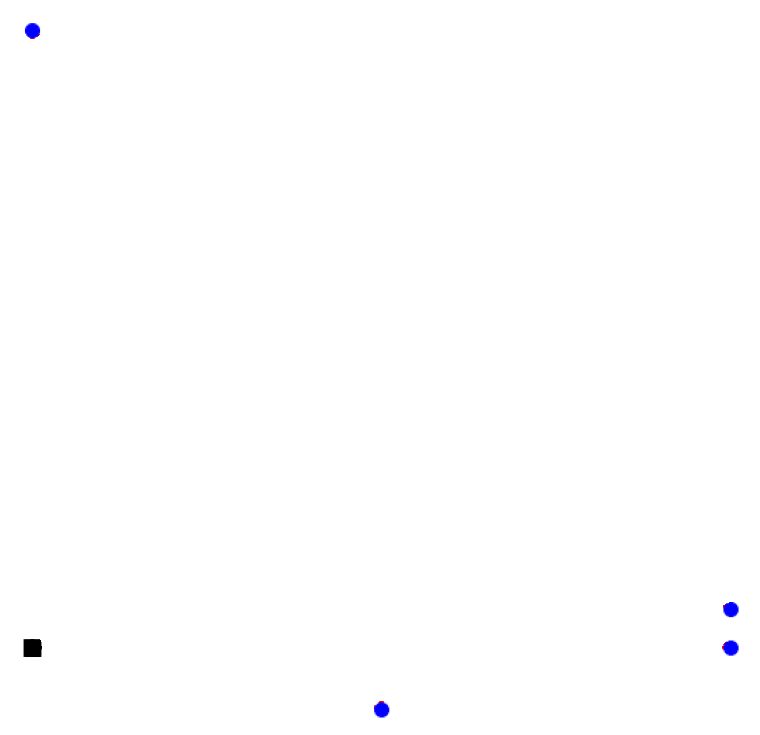
\includegraphics[width=0.37\linewidth]{poikonen_2}
			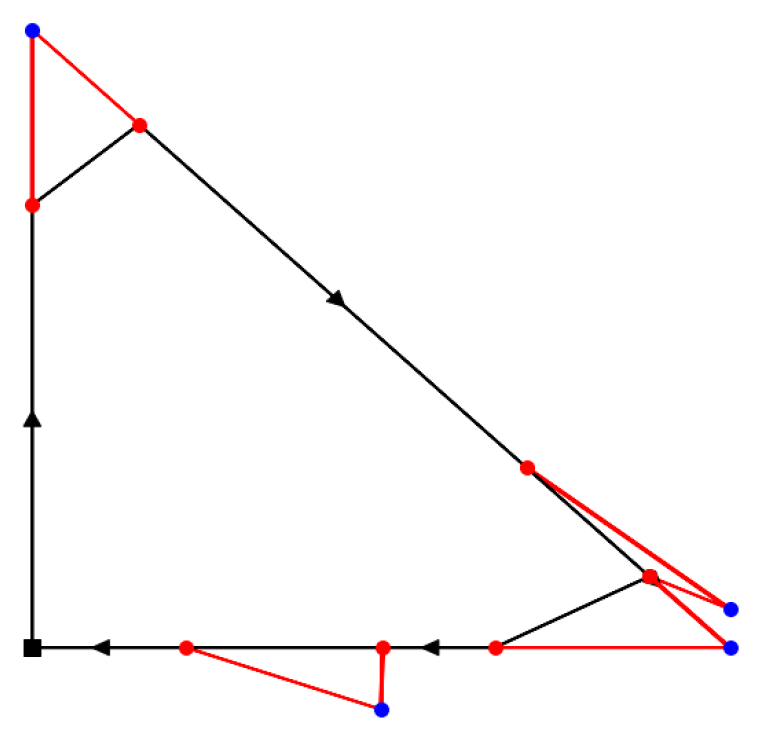
\includegraphics[width=0.37\linewidth]{poikonen_1}
		\end{center}
	\end{frame}
	
	\begin{frame}{Problem Description}
	\begin{itemize}
	    \item There is one mothership and one drone in coordination to visit a set of target graphs, whose locations are given.
	    \item For each graph $g\in\mathcal G$ the drone performs the following task:
	    \begin{enumerate}
	        \item It is launched from the current mothership location (to be determined).
	        \item It flies to the graph $g$ that has to be visited.
	        \item It traverses the required edges of graph $g$.
	        \item It returns to the current position of the mothership (to be determined).
	    \end{enumerate}
	    We assume wlog that the mothership and the drone do not need to arrive at each rendezvous location at the same time: the fastest arriving vehicle may wait for the other at the rendezvous point.
	\end{itemize}
	\end{frame}
	
	\begin{frame}{Problem Description}
	It is required to determine:
	    \begin{itemize}
	        \item The tour of the mothership starting at $orig$, deciding the different launching and rendezvous points, and returning to $dest$.
	        \item The order of visits of the target graphs followed by the drone, determining the corresponding launching and rendezvous points of the drone on each visited graph.
	        \item The tour followed by the drone on each target graph $g \in \mathcal{G}$.
	    \end{itemize}
	\end{frame}
	
	\begin{frame}{Problem Description}
	    Depending on the assumptions made on the movements of the mothership vehicle, this problem gives rise to two different versions: 
	    \begin{itemize}
	        \item The mothership vehicle can move freely on the continuous space (all terrain ground vehicle, boat on the water or aircraft vehicle), called the All terrain Mothership-Drone Routing Problem with Graphs (AMDRPG).
	        \item The mothership can move on a connected piecewise linear polygonal chain, called the Network Mothership-Drone Routing Problem on a Polygonal with Graphs (PMDRPG).
	        \item The mothership can move on a road network (that is, it is a normal truck or van), called the Network Mothership-Drone Routing Problem with Graphs (NMDRPG).
	    \end{itemize}
	\end{frame}
	
	\begin{frame}{Parameters of the AMDRPG}
	The known parameters of the problem are:
	\begin{itemize}
	    \item $orig$: coordinates of the point defining the origin of the mothership path (or tour).
        \item $dest$: coordinates of the point defining the destination of the mothership path (or tour).
        \item $\mathcal{G}$: set of the target graphs.\\
        \item $g = (V_g, E_g)$: set of nodes and edges of each target graph $g \in \mathcal{G}$.
        \item $\mathcal{L}(e_g)$: length of edge $e$ of graph $g \in \mathcal{G}$.
        \item $B^{e_g}, C^{e_g}$: coordinates of the endpoints of edge $e$ of graph $g \in \mathcal{G}$.
        \item $\alpha^{e_g}$: percentage of edge $e$ of graph $g \in \mathcal{G}$ that must be visited.
        \item $\alpha^g$: percentage of graph $g \in \mathcal{G}$ that must be visited.
        \item $v_D$: drone speed.
        \item $v_M$: mothership speed.
        \item $M$: big-M constant.
    \end{itemize}
	\end{frame}
	
	\begin{frame}{Initial data for the AMDRPG}
	    \begin{center}
			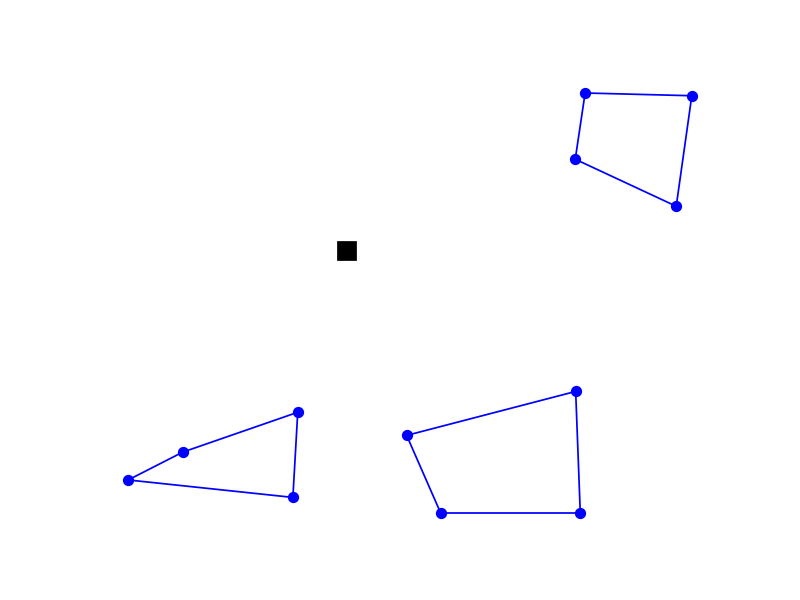
\includegraphics[width=0.7\linewidth]{PDMTZ_1}
		\end{center}
	\end{frame}
	
	\begin{frame}{Binary and Integer Decision Variables for the AMDRPG-ST}
	\begin{itemize}
	    \item $\mu^{e_g} \in \{0,1\} \:\: \forall e_g \in E_g$ ($g \in \mathcal{G}$): equal to 1 if edge $e$ of graph $g$ (or a portion of it) is visited by the drone, and  0 otherwise.
        \item $entry^{e_g} \in \{0,1\} \:\: \forall e_g \in E_g$ ($g \in \mathcal{G}$): auxiliary binary variable used for linearizing expressions.
        \item $u^{e_{g}t} \in \{0,1\} \:\: \forall e_g \in E_g$ ($g \in \mathcal{G}$) $\: \forall t \in T$: equal to 1 if the drone enters in graph $g$ by $e_g$ at stage $t$, 0 otherwise.
        \item $z^{e_{g}e^{'}_{g}} \in \{0,1\} \:\: \forall e_g, e_g' \in E_g$ ($g \in \mathcal{G}$): equal to 1 if the drone goes from $e_g$ to $e^{'}_{g}$, 0 otherwise.
        \item $v^{e_{g}t} \in \{0,1\} \:\: \forall e_g \in E_g$ ($g \in \mathcal{G}$) $\: \forall t \in T$: equal to 1 if the drone exits from graph $g$ by $e_g$ at stage $t$, 0 otherwise.
        \item $s^{e_g},\; \forall e_g \in E_g$ ($g \in \mathcal{G}$): integer non negative variable representing the order of visit of edge $e$.
    \end{itemize}
	\end{frame}
	
	\begin{frame}{Continuous Decision Variables for the AMDRPG-ST}
	\textbf{Location variables}
	\begin{itemize}
	    \item $\rho^{e_g} \in [0,1]$ and $\lambda^{e_g} \in [0,1] \:\: \forall e_g \in E_g$ ($g \in \mathcal{G}$): defining the entry and exit points on $e_g$.
        \item $\nu_\text{min}^{e_g}$ and $\nu_\text{max}^{e_g} \in [0,1] \forall e_g \in E_g$ ($g \in \mathcal{G}$): auxiliary variables used for linearizing expressions.
        \item $x_L^t \:\: \forall t \in T$: coordinates representing the point where the mothership launches the drone at stage $t$.
        \item $x_R^t \:\: \forall t \in T$: coordinates representing the point where the mothership retrieves the drone at stage $t$.
        \item $R^{e_g} \:\: \forall e_g \in E_g$ ($g \in \mathcal{G}$): coordinates representing the entry point on edge $e$ of graph $g$.
        \item $L^{e_g} \:\: \forall e_g \in E_g$ ($g \in \mathcal{G})$: coordinates representing the exit point on edge $e$ of graph $g$.
    \end{itemize}
    \end{frame}
    
    \begin{frame}{Continuous Decision Variables for the AMDRPG-ST}
    \textbf{Distance variables}
    \begin{itemize}
        \small
        \item $d_L^{e_gt} \geq 0, \:\: \forall e_g \in E_g$ ($g \in \mathcal{G}$) $\forall t \in T$: representing the distance travelled by the drone from the launching point $x_L^t$ on the mothership at stage $t$ to the first visiting point $R^{e_g}$ on $e_g$.
        \item $d^{e_ge^\prime_g} \geq 0, \:\: \forall e_g, e^\prime_g \in E_g $ ($g \in \mathcal{G}$): representing the distance travelled by the drone from the launching
        point $L^{e_g}$ on $e_g$ to the rendezvous point $R^{e^\prime_g}$ on $e^\prime_g$.
        \item $d^{e_g} \geq 0, \:\: \forall e_g \in E_g$ ($g \in \mathcal{G}$): representing the distance travelled by the drone from the rendezvous point $R^{e_g}$ to the launching point $L^{e_g}$ on $e_g$. 
        \item $d_R^{e_gt} \geq 0 \:\: \forall e_g \in E_g$ ($g \in \mathcal{G}$) $\forall t \in T$: representing the distance travelled by the drone from the last
        visiting point $L^{e_g}$ on $e_g$ to the rendezvous point $x_R^t$ on the mothership at stage $t$.
        \item $d_{LR}^t \geq 0 \:\: \forall t \in T$: representing the distance travelled by the mothership from the launching point $x_L^t$ to the rendezvous point $x_R^t$ at stage $t$.
        \item $d_{RL}^t \geq 0 \:\: \forall t \in T$: representing the distance travelled by the mothership from the rendezvous point $x_R^t$ at stage $t$ to the launching point $x_L^{(t+1)}$ at the stage $t+1$.
    \end{itemize}
	\end{frame}

    	\begin{frame}{Visit of the graphs}
	    We have considered two modes of visit to the target graphs $g\in \mathcal{G}$ that must be represented by their corresponding constraints:
        \begin{itemize}
            \item Visiting a percentage $\alpha^{e_g}$ of each edge $e_g$ which can be modeled by:
            \begin{equation}\label{eq:alphaE}\tag{$\alpha$-E}
            |\lambda^{e_g} - \rho^{e_g}|\mu^{e_g}\geq \alpha^{e_g}, \quad \forall e_g\in E_g.
            \end{equation}
            \item Visiting a percentage $\alpha^g$ of the total length $\mathcal L(g)$ of the graph $g$ modeled by:
            \begin{equation}\label{eq:alphaG}\tag{$\alpha$-G}
            \sum_{e_g\in E_g} \mu^{e_g}|\lambda^{e_g} - \rho^{e_g}|\mathcal L(e_g) \geq \alpha^g\mathcal L(g).
            \end{equation}
            %where $\mathcal L(g)$ denotes the total length of the graph.
        \end{itemize}
	\end{frame}
	
	\begin{frame}{Visit of the graphs}
	    In both cases the corresponding constraints are nonlinear. For each edge $e_g$, we linearize the absolute value constraint \eqref{eq:alphaE} by introducing a binary variable:
        \begin{equation}\label{eq:alpha-E}\tag{$\alpha$-E}
         \mu^{e_g}|\rho^{e_g}-\lambda^{e_g}|\geq \alpha^{e_g} \Longleftrightarrow
         \left\{
         \begin{array}{ccl}
          \rho^{e_g} - \lambda^{e_g}                       & =    & \nu_\text{max}^{e_g} - \nu_\text{min}^{e_g}                                     \\
          \nu_\text{max}^{e_g}                         & \leq & 1-{\text{entry}^{e_g}}                                    \\
          \nu_\text{min}^{e_g}                      & \leq & {  \text{entry}^{e_g}},                                        \\
          \mu^{e_g}(\nu_\text{max}^{e_g} + \nu_\text{min}^{e_g} ) & \geq & \alpha^{e_g}.
          \\
         \end{array}
         \right.
        \end{equation}
        
        \noindent
        The linearization of \eqref{eq:alphaG} is similar to \eqref{eq:alphaE} and only requires changing the last inequality in \eqref{eq:alpha-E} for
        
        \begin{equation}\label{eq:alpha-G}\tag{$\alpha$-G}
        \sum_{e_g\in E_g} \mu^{e_g}(\nu_\text{max}^{e_g} + \nu_\text{min}^{e_g})\mathcal L(e_g)\geq \alpha_g\mathcal L(g).
        \end{equation}
	\end{frame}
	
	\begin{frame}{Modeling the Drone Route}
	\begin{small}

	\begin{align}
        \sum_{g\in \mathcal G}\sum_{e_g\in E_g} u^{e_gt} & = 1, &\forall t\in T \label{st:DEnt},\\%\tag{DEn}\\
        \sum_{g\in\mathcal G}\sum_{e_g\in E_g} v^{e_gt} & = 1, &\forall t\in T, \label{st:DExt}\\%\tag{DEx}\\
        \sum_{e_g\in E_g} \sum_{t\in T} u^{e_gt} & = 1, &\forall g\in\mathcal G, \label{st:DEng}\\%\tag{D
        \sum_{e_g\in E_g}\sum_{t\in T} v^{e_gt} & = 1, &\forall g\in\mathcal G, \label{st:DExg}\\%\tag{D
        \sum_{e_g\in E_g} u^{e_gt} & = \sum_{e_g\in E_g} v^{e_gt}, &\forall g\in\mathcal G, \forall t\in T, \label{st:Duv}\\%\tag{D
        \sum_{e^\prime_g\in E_g} z_g^{e^\prime_ge_g} + \sum_{t\in T} u^{e_gt} & = \mu^{e_g}, &\forall e_g\in E_g:g\in\mathcal G, \label{st:DInu}\\
        \sum_{e^\prime_g\in E_g} z_g^{e_ge^\prime_g} + \sum_{t\in T} v^{e_gt} & = \mu^{e_g}, &\forall e_g\in E_g:g\in\mathcal G. \label{st:DInv}
    \end{align}
    \end{small}
	\end{frame}
	
	\begin{frame}{Subtour elimination inside the graph}
	    \begin{small}
		To prevent the existence of subtours within each graph $g\in \mathcal G$ that the drone must visit: 
		\begin{itemize}
		\item One can add the Miller-Tucker-Zemlin constraints, given by:
    		\begin{align}
    		    s^{e_g} - s^{e^\prime_g} + |E_g|z^{e_ge^\prime_g} & \leq |E_g| - 1  , &\quad\forall e_g \neq e_g'\in E_g \tag{MTZ$_1$}, \label{MTZ1}\\
                0 & \leq s^{e_g} \leq |E_g| - 1 &\quad\forall e_g\in E_g\tag{MTZ$_2$},\label{MTZ2}
                \end{align}
        \item It is also possible to include the subtour elimination constraints:
        \begin{equation}\tag{SEC}\label{SEC}
        \sum_{e_g, e^\prime_g \in S} z_g^{e_ge^\prime_g} \leq |S| - 1, \quad \forall S\subset E_g:g\in \mathcal G.
    \end{equation}
    \end{itemize}
    \end{small}
	    
	\end{frame}
	
	\begin{frame}{Distance constraints}
	    To account for the different distances among the decision variables of the model we need to set the continuous variables $d_L^{e_gt}$, $d^{e_g}$, $d^{e_ge^\prime_g}$, $d_R^{e_gt}$, $d_{RL}^t$ and $d_{LR}^t$. This can be done by means of the following constraints:
        
        \begin{align*}
        \|x_L^t- R^{e_g}\| & \leq  d_L^{e_gt},  &\quad \forall e_g:g\in \mathcal{G}, \forall t\in T \tag{DIST$_{1}$-t}, \label{eq:d1}\\
        \|R^{e_g}- L^{e_g}\| & \leq  d^{e_g},  &\quad \forall e_g:g\in \mathcal{G},\forall t\in T \tag{DIST$_{2}$-t}, \label{eq:d2}\\
        \|R^{e_g}- L^{e^\prime_g}\| & \leq  d^{e_ge^\prime_g}, &\quad \forall e_g\neq e_g'\in E_g:g\in \mathcal{G} \tag{DIST$_{3}$-t}, \label{eq:d3}\\
        \|L^{e_g}- x_R^t\| & \leq  d_R^{e_gt}, &\quad \forall e_g:g\in \mathcal{G},\forall t\in T \tag{DIST$_{4}$-t}, \label{eq:d4}\\
        \|x_R^t- x_L^{t+1}\| & \leq  d_{RL}^t, & \quad \forall t\in T, \tag{DIST$_{5}$-t} \label{eq:d5}\\
        \|x_L^t- x_R^t\| & \leq  d_{LR}^t, & \quad \forall t\in T. \tag{DIST$_{6}$-t} \label{eq:d6}\\
        \end{align*}
	\end{frame}
	
	\begin{frame}{Coordination constraint}
	    To ensure that the time spent by the drone to visit graph $g$ at stage $t$ is less than or equal to the time that the mothership needs to move from the launching point to the rendezvous point at stage $t$, we need to define the following coordination constraint for each $g\in \mathcal G$ and $t\in T$:

        \begin{equation}\tag{DCW-t}\label{DCW-t}
        \tiny
        \frac{1}{v_D}\left(\sum_{e_g\in E_g} u^{e_gt}d_L^{e_gt} + \sum_{e_g, e^\prime_g\in E_g}z^{e_ge^\prime_g}d^{e_ge^\prime_g} + \sum_{e_g\in E_g} \mu^{e_g}d^{e_g} + \sum_{e_g\in E_g} v^{e_gt}d_R^{e_gt}\right) \leq \frac{d_{RL}^t}{v_M} + M(1 - \sum_{e_g\in E_g} u^{e_gt}).
        \end{equation}
	\end{frame}
	
	\begin{frame}{Setting the origin and the destination}
	    Eventually, we have to impose that the tour of the mothership, together with the drone, starts from the origin $orig$ and ends at the destination $dest$. To this end, we define the following constraints:

        \begin{align*}
        x_L^0 & =  orig,  \tag{ORIG$_1$} \label{eq:O1} \\
        x_R^0 & =  orig,  \tag{ORIG$_2$} \label{eq:O2} \\
        x_L^{|\mathcal{G}|+1} & =  dest,  \tag{DEST$_1$} \label{eq:D1} \\
        x_R^{|\mathcal{G}|+1} & =  dest.  \tag{DEST$_2$} \label{eq:D2} 
        \end{align*}

	\end{frame}
	
	\begin{frame}{Formulation for the AMDRPG-ST}
	
	\begin{align*}
	    \text{min}\quad &\sum_{g\in\mathcal G}\sum_{e_g\in E_g}\sum_{t\in T} (u^{e_gt}d_L^{e_gt} + v^{e_gt}d_R^{e_gt}) + \sum_{g\in\mathcal G}\sum_{e_g\in E_g} \mu^{e_g}d^{e_g} + \\
	    + & \sum_{g\in\mathcal G}\sum_{e_g,e^\prime_g\in E_g}z^{e_ge^\prime_g}d^{e_ge^\prime_g} + \sum_{t\in T} (d_{RL}^t + d_{LR}^t) \\
	    \text{s.t.}\quad & \eqref{st:DEnt}-\eqref{st:DInv}, \\
	    & \eqref{MTZ1} - \eqref{MTZ2} \text{ or } \eqref{SEC}, \\
	    & \eqref{eq:alpha-E} \text{ or } \eqref{eq:alpha-G}, \\
	    & \eqref{DCW-t}, \\
	    & \eqref{eq:d1}-\eqref{eq:d6}, \\
	    & \eqref{eq:O1}-\eqref{eq:D2}.
	\end{align*}
% 	\begin{mini*}|s|
%          {}{\sum_{g\in\mathcal G}\sum_{e_g\in E_g}\sum_{t\in T} (u^{e_gt}d_L^{e_gt} + v^{e_gt}d_R^{e_gt}) + \sum_{g\in\mathcal G}\sum_{e_g\in E_g} \mu^{e_g}d^{e_g} +
%          \breakObjective{\sum_{g\in\mathcal G}\sum_{e_g,e^\prime_g\in E_g}z^{e_ge^\prime_g}d^{e_ge^\prime_g} + \sum_{t\in T} (d_{RL}^t + d_{LR}^t)}}{}{} \label{AMDRPG-ST} \tag{AMDRPG-ST}
%          \addConstraint{\eqref{st:DEnt}-\eqref{st:DInv}}{}{}
%          \addConstraint{\eqref{MTZ1} - \eqref{MTZ2} \text{ or } \eqref{SEC} }{}{}
%          \addConstraint{\eqref{eq:alpha-E} \text{ or } \eqref{eq:alpha-G}}{}{}
%          \addConstraint{\eqref{DCW-t}}{}{}
%          \addConstraint{\eqref{eq:d1}-\eqref{eq:d6}}{}{}
%          \addConstraint{\eqref{eq:O1}-\eqref{eq:D2}}.{}{}
%     \end{mini*}
	    
	\end{frame}
	
	\begin{frame}{Alternative formulations based on enforcing connectivity}
	    In this family of formulations we replace the variables $u^{\cdot t}, v^{\cdot t}$ and constraints that model the tour using stages, namely (1)-(7), by constraints that ensure connectivity.
	    
	    \bigskip
	    
	    We will distinguish two different approaches:
    	\begin{itemize}
    		\item Using Miller-Tucker-Zemlin compact formulation.
    		\item Using the known subtour elimination constraints.
    	\end{itemize}
	\end{frame}
	
	\begin{frame}{\large Binary and Integer Decision Variables for the AMDRPG-MTZ}
	\begin{itemize}
	    \small
	    \item $\mu^{e_g} \in \{0,1\} \:\: \forall e_g \in E_g$ ($g \in \mathcal{G}$): equal to 1 if edge $e$ of graph $g$ (or a portion of it) is visited by the drone, and 0 otherwise.
        \item $entry^{e_g} \in \{0,1\} \:\: \forall e_g \in E_g$ ($g \in \mathcal{G}$): auxiliary binary variables for linearization.
        \item $u^{e_{g}} \in \{0,1\} \:\: \forall e_g \in E_g$ ($g \in \mathcal{G}$): equal to 1 if the drone enters in graph $g$ by $e_g$, 0 otherwise.
        \item $z^{e_{g}e^{'}_{g}} \in \{0,1\} \:\: \forall e_g, e_g' \in E_g$ ($g \in \mathcal{G}$): equal to 1 if the drone goes from $e_g$ to $e^{'}_{g}$, 0 otherwise.
        \item $v^{e_{g}} \in \{0,1\} \:\: \forall e_g \in E_g$ ($g \in \mathcal{G}$): equal to 1 if the drone exits from graph $g$ by $e_g$, 0 otherwise.
        \item $w^{gg'} \in \{0,1\} \:\:\ \forall g,g' \in \mathcal{G}$: equal to 1 if the mothership moves from $x_R^g$ to $x_L^{g^'}$, 0 otherwise.
        \item $s^{e_g} \:\: \forall e_g \in E_g$ ($g \in \mathcal{G}$): integer non negative variables representing the order of visit of edge $e$ of graph $g$.
    \end{itemize}
	\end{frame}
	
	\begin{frame}{Continuous Decision Variables for the AMDRPG-MTZ}
	\textbf{Location variables}
	\begin{itemize}
        \item $\rho^{e_g} \in [0,1]$ and $\lambda^{e_g} \in [0,1] \:\: \forall e_g \in E_g$ ($g \in \mathcal{G}$): defining the entry and exit points on $e_g$.
        \item $\nu_\text{min}^{e_g}$ and $\nu_\text{max}^{e_g} \in [0,1] \:\: \forall e_g \in E_g$ ($g \in \mathcal{G}$): auxiliary variables for linearization.
        \item $x_L^g \:\: \forall g \in \mathcal{G}$: pairs of coordinates representing the point where the mothership launches the drone to visit graph $g$.
        \item $x_R^g \:\: \forall g \in \mathcal{G}$: pairs of coordinates representing the point where the mothership retrieves the drone after visit graph $g$.
        \item $R^{e_g} \:\: \forall e_g \in E_g$ ($g \in \mathcal{G}$): coordinates representing the entry point on edge $e$ of graph $g$.
        \item $L^{e_g} \:\: \forall e_g \in E_g$ ($g \in \mathcal{G}$): coordinates representing the exit point on edge $e$ of graph $g$.
    \end{itemize}
    \end{frame}
    
    \begin{frame}{Continuous Decision Variables for the AMDRPG-MTZ}
    \textbf{Distance variables}
    \begin{itemize}
        \footnotesize
        \item $d_L^{e_g} \geq 0 \:\: \forall e_g \in E_g$ ($g \in \mathcal{G}$): representing the distance travelled by the drone from the launching point 
         on the mothership  $x_L^g$ to the first visiting point $R^{e_g}$ on edge $e_g$.
        \item $d^{e_ge^\prime_g} \geq 0 \:\: \forall e_g, e^\prime_g \in E_g $ ($g \in \mathcal{G}$): representing the distance travelled by the drone from launching point 
        \item $L^{e_g}$ on $e_g$ to the rendezvous point $R^{e^\prime_g}$ on $e^\prime_g$.
        \item $d^{e_g} \geq 0 \:\: \forall e_g \in E_g$ ($g \in \mathcal{G}$): representing the distance travelled by the drone from the rendezvous point
$R^{e_g}$ to the launching point $L^{e_g}$ on $e_g$. 
        \item $d_R^{e_g} \geq 0 \:\: \forall e_g \in E_g$ ($g \in \mathcal{G}$): representing the distance travelled by the drone from the last visiting point
 $L^{e_g}$ on $e_g$ to the rendezvous point $x_R^g$ on the mothership.
        \item $d_{LR}^g \geq 0 \:\: \forall g \in \mathcal{G}$: representing the distance travelled by the mothership from the launching point
 $x_L^g$ to the rendezvous point $x_R^g$ while the drone is visiting $g$.
        \item $d_{RL}^{gg_\prime} \geq 0 \:\: \forall g, g^{'} \in \mathcal{G}$: representing the distance travelled by the mothership from the 
rendezvous point $x_R^g$ for graph $g$ to the launching point $x_L^{g\prime}$ for graph $g\prime$.
    \end{itemize}
	\end{frame}
	
	\begin{frame}{Modeling the Drone Route}
	We can model the route that the drone follows in each particular graph $g\in \mathcal G$:
	\begin{align}
        \sum_{e_g\in E_g} u^{e_g} & = 1, & \quad\forall g \in \mathcal G, \label{DEnt2}\\%\tag{DEn}\\
        \sum_{e_g\in E_g} v^{e_g} & = 1, & \quad\forall g \in \mathcal G, \label{DExt}\\%\tag{DEx}\\
        \sum_{e^\prime_g\in E_g} z^{e_g'e_g} + u^{e_g} & = \mu^{e_g}, &\quad\forall e_g\in E_g:g\in\mathcal G, \label{DInu}\\
        \sum_{e^\prime_g\in E_g} z^{e_ge^_g'} + v^{e_g} & = \mu^{e_g}, &\quad\forall e_g\in E_g:g\in\mathcal G. \label{DInv2}
    \end{align}
	\end{frame}
	
	\begin{frame}{Modeling the Mothership Route}
	On the other hand, to Mode the tour followed by the mothership, we have to include the following new constraints:
	    \begin{align}
	        \small
            \sum_{g\in\mathcal G} w^{g0} & = 0, \label{TOrig}\\
            \sum_{g'\in\mathcal G} w^{(n_G+1) g'} & = 0, \label{TDest}\\
            \sum_{g'\in\mathcal G\setminus\{g\}} w^{gg'} & = 1, \label{TExt} &\quad\forall g\in \mathcal G,\\
            \sum_{g\in\mathcal G\setminus\{g'\}} w^{gg'} & = 1, &\quad\forall g'\in \mathcal G,\label{TEnt}\\
            s_g - s_{g'} + |\mathcal G|w^{gg'} & \leq |\mathcal G| - 1  , &\quad\forall g \neq g', \tag{MTZ$_3$} \label{MTZ3}\\
            0 & \leq s_g \leq |\mathcal G| - 1 &\quad\forall g\in \mathcal G,\tag{MTZ$_4$}\label{MTZ4}\\
            s_0 & = 0, \tag{MTZ$_5$}\label{MTZ5}\\
            s_{n_G+1}&=n_G+1. \tag{MTZ$_6$}\label{MTZ6}
        \end{align}
	\end{frame}
	
	\begin{frame}{Distance Constraints}
	    \begin{align*}
        \|x_L^g- R^{e_g}\| &\leq d_L^{e_g},&\quad \forall e_g:g\in\mathcal G, \tag{DIST$_{1}$-g} \label{eq:d1g}\\
        \|R^{e_g}- L^{e_g}\| &\leq d^{e_g},&\quad \forall e_g:g\in\mathcal G, \tag{DIST$_{2}$-g}\\
        \|R^{e_g}- L^{e^\prime_g}\| &\leq d^{e_ge^\prime_g},&\quad \forall e_g\neq e'_g:g\in\mathcal G, \tag{DIST$_{3}$-g}\\
         \|L^{e_g}- x_R^g\| &\leq d_R^{e_g},&\quad \forall e_g:g\in\mathcal G, \tag{DIST$_{4}$-g}\\
        \|x_R^g- x_L^{g'}\| &\leq d^{gg'}_{RL},& \quad \forall g,g'\in\mathcal G, \tag{DIST$_{5}$-g}\\
        \|x_L^g- x_R^g\| &\leq d^g_{LR},& \quad \forall g\in\mathcal G. \tag{DIST$_{6}$-g} \label{eq:d6g}\\
        \end{align*}
	\end{frame}
	
	\begin{frame}{Coordination constraint}
	    Again, we need to be sure that the time spent by the drone to visit the graph $g$ is less than or equal to the time that the mothership needs to move from the launching point to the rendezvous point associated to this graph $g$. Hence, by using the same argument, as the one used in \eqref{DCW-t}, we define for each $g\in \mathcal G$:
        \begin{equation}
        \footnotesize
         \frac{1}{v_D}\left(\sum_{e_g\in E_g} u^{e_g}d_L^{e_g} + \sum_{e_g, e^\prime_g\in E_g}z^{e_ge^\prime_g}d^{e_ge^\prime_g} + \sum_{e_g\in E_g} \mu^{e_g} d^{e_g} + \sum_{e_g\in E_g}v^{e_g}d_R^{e_g}\right)\leq \frac{d_{RL}^{g}}{v_M}, \quad\forall g\in\mathcal G.\label{DCW-g}\tag{DCW-g}
        \end{equation}

	\end{frame}
	
	\begin{frame}{Formulation for the AMDRPG-MTZ (resp. SEC)}
	\begin{footnotesize}
	\begin{align*}
	    \text{min}\quad &\sum_{g\in\mathcal G}\sum_{e_g\in E_g} (u^{e_g}d_L^{e_g} + v^{e_g}d_R^{e_g}) + \sum_{g\in\mathcal G}\sum_{e_g\in E_g} \mu^{e_g} d^{e_g} + \\
	    + & \sum_{g\in\mathcal G}\sum_{e_g,e^\prime_g\in E_g}z^{e_ge^\prime_g}d^{e_ge^\prime_g} + \sum_{g\in\mathcal G} d_{LR}^g + \sum_{g,g'\in \mathcal G}d_{RL}^{gg'}w^{gg'} \\
	    \text{s.t.}\quad & \eqref{DEnt2}-\eqref{TEnt}, \\
	    & \eqref{MTZ1} - \eqref{MTZ2} \text{ or } \eqref{SEC}, \\
	    & \eqref{MTZ3} - \eqref{MTZ6}, \\
	    & \eqref{eq:alpha-E} \text{ or } \eqref{eq:alpha-G}, \\
	    & \eqref{DCW-g}, \\
	    & \eqref{eq:d1g}-\eqref{eq:d6g}, \\
	    & \eqref{eq:O1}-\eqref{eq:D2}.
	\end{align*}
	\end{footnotesize}
	The formulation above can be slightly modified replacing constraints $\eqref{MTZ3} - \eqref{MTZ6}$ by
    \begin{equation}\label{SEC-graph}
    \sum_{g,g'\in \mathcal G} w^{gg'} \le |S|-1, \quad \forall S\subseteq \{1,\ldots, |\mathcal G|\}.
    \end{equation}

	\end{frame}
	
	\begin{frame}{Example 1}
    \begin{figure}
        \centering
        \subfigure{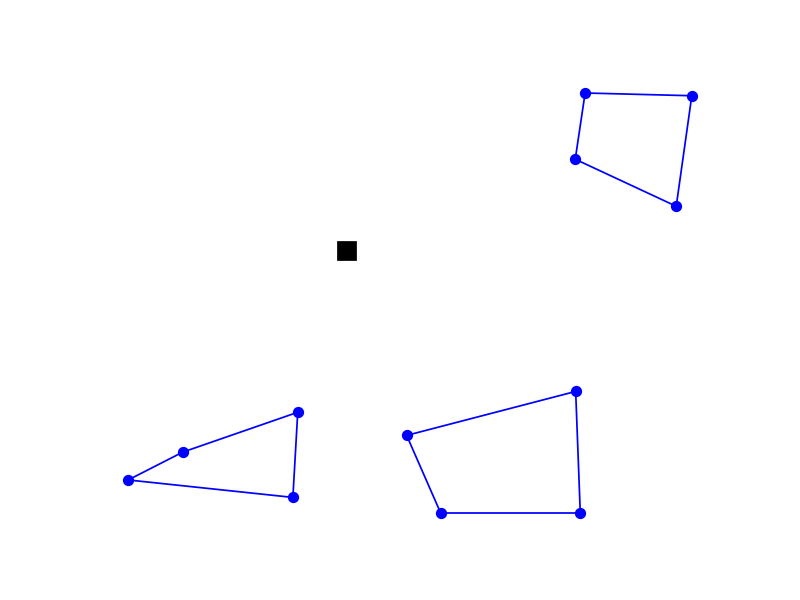
\includegraphics[width=0.28\textwidth]{PDMTZ_1.png}} 
        \subfigure{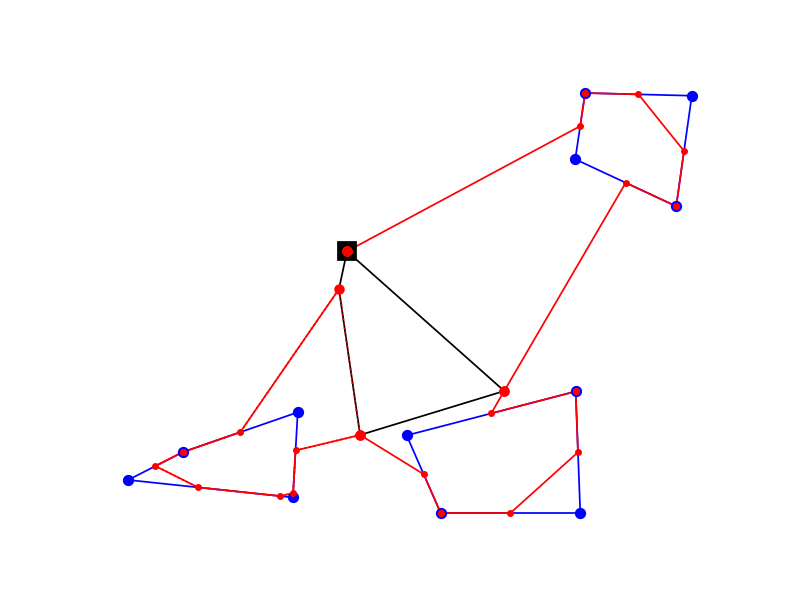
\includegraphics[width=0.28\textwidth]{PDMTZ_e.png}} 
        \subfigure{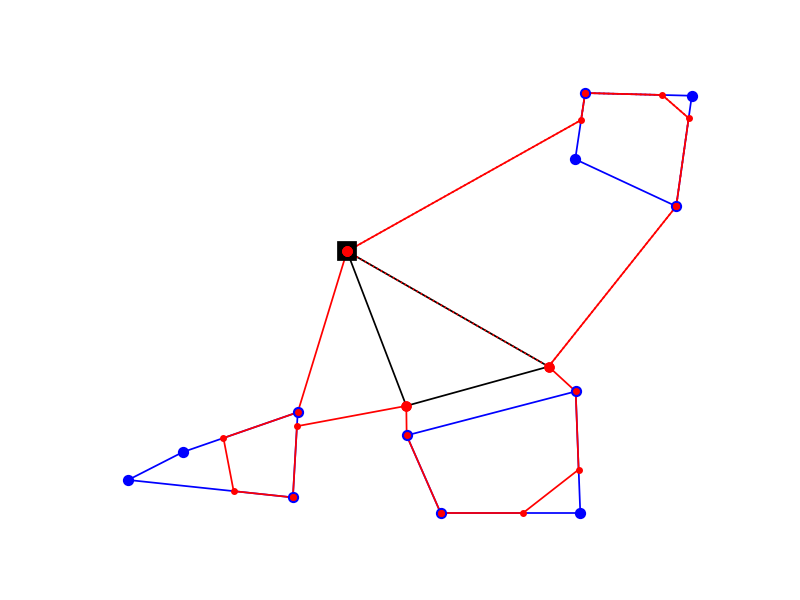
\includegraphics[width=0.28\textwidth]{PDMTZ_g.png}}
        \caption{(a) Origin and target graphs, (b) Visit of $\alpha^{e_g}\%$ of each edge, (c) Visit of $\alpha_g\%$ of each graph.}
        \label{fig:illustrative}
    \end{figure}	
    \end{frame}
    
    \begin{frame}{Example 2: Percentage of each edge}
    	\begin{center}
			\animategraphics[controls, width = 0.7\linewidth]{3}{gif_mdrpg_alphae/}{0}{20}
		\end{center}
    \end{frame}

    \begin{frame}{Example 3: Percentage of each graph}
    	\begin{center}
			\animategraphics[controls, width = 0.7\linewidth]{3}{gif_mdrpg_alphag/}{0}{20}
		\end{center}
    \end{frame}
	
	\begin{frame}{Parameters of the NMDRPG}
		\begin{itemize}
        \item \textcolor{red}{$\mathcal N=(V, E)$: set of nodes and edges of the network representing the road system where the mothership can move.}
        \item $e=(i,j)$,$e'=(i',j')$: starting edge and ending edge of the mothership tour.
        \item $\mathcal{G}$: set of the target graphs.
        \item $g = (V_g, E_g)$: set of nodes and edges of each target graph $g \in \mathcal{G}$.
        \item $\mathcal{L}(e_g)$: length of edge $e$ of graph $g \in \mathcal{G}$.
        \item $B^{e_g}, C^{e_g}$: coordinates of the endpoints of edge $e$ of graph $g \in \mathcal{G}$.
        \item $\alpha^{e_g}$: percentage of edge $e$ of graph $g \in \mathcal{G}$ that must be visited.
        \item $\alpha^g$: percentage of graph $g \in \mathcal{G}$ that must be visited.
        \item $v_D$: drone speed.
        \item $v_M$: mothership speed.
        \item $M$: big-M constant.
    \end{itemize}
	    
	    
	\end{frame}
	
	\begin{frame}{Binary and Integer Decision Variables for the NMDRPG-ST}
	\textbf{Drone tour variables}
	\begin{itemize}
	    \item $\mu^{e_g} \in \{0,1\} \:\: \forall e_g \in E_g$ ($g \in \mathcal{G}$): equal to 1 if edge $e$ of graph $g$ (or a portion of it) is visited by the drone,  and 0 otherwise.
        \item $entry^{e_g} \in \{0,1\} \:\: \forall e_g \in E_g$ ($g \in \mathcal{G}$): auxiliary binary variables for linearization.
        \item $u^{e_{g}t} \in \{0,1\} \:\: \forall e_g \in E_g$ ($g \in \mathcal{G}$), $\:\: \forall t \in T$: equal to 1 if the drone enters in graph $g$ by $e_g$ at stage $t$,   0 otherwise.
        \item $z^{e_{g}e^{'}_{g}} \in \{0,1\} \:\: \forall e_g, e_{g'} \in E_g$ ($g \in \mathcal{G}$): equal to 1 if the drone goes from $e_g$ to $e^{'}_{g}$, 0 otherwise.
        \item $v^{e_{g}t} \in \{0,1\} \:\: \forall e_g \in E_g$ ($g \in \mathcal{G}$), $\:\: \forall t \in T$: equal to 1 if the drone exits from graph $g$ by $e_g$ at stage $t$,  0 otherwise.
        \item $s^{e_g} \:\:\ \forall e_g \in E_g$ ($g \in \mathcal{G}$): integer non negative variable representing the order of visit of edge $e$ of graph $g$.
    \end{itemize}
    \end{frame}
    
    \begin{frame}{Binary and Integer Decision Variables for the NDMRPG-ST}
    \textbf{Mothership tour variables inside the network}

    \begin{itemize}
        \color{red}{
        \item $\mu_{L}^{et} \in \{0,1\}, \:\: \forall e \in E, \:\:\ \forall t \in T$: equal to 1 if the launching point $x_L^t$ is located on $e$ at stage $t$.
        \item $\mu_{R}^{et} \in \{0,1\}, \:\: \forall e \in E, \:\:\ \forall t \in T$: equal to 1 if the rendezvous point $x_R^t$ is located on $e$ at stage $t$. 
        \item $z_{LR}^{ee't} \in \{0,1\} \:\:\ \forall e,e' \in E, \:\:\ \forall t \in T$: equal to 1 if the launching point $x_L^t$ is located on $e$ and the rendezvous point $x_R^t$ is located on $e^{\prime}$ at stage $t$. 
        \item $b_{LR}^{it} \in \{0,1\}, \:\: \forall i: e=(i,j) \in E, \:\:\ \forall t \in T$, equal to 1 if the mothership exits from $x_L^t$ by the vertex $V^i$ of the edge $e$.
        \item $c_{LR}^{it} \in \{0,1\}, \:\: \forall i: e=(i,j) \in E, \:\:\ \forall t \in T$, equal to 1 if the mothership enters in $x_R^t$ by the vertex $V^i$ of the edge $e$.
        \item $q_{LR}^{et}\geq 0 \:\:\ \forall e \in E, \:\: \forall t \in T$, integer variable counting the number of times the mothership fully  traverses edge $e$ to move between the launching point $x_L^t$ on $e$ to the rendezvous point $x_R^t$   on $e'$ at stage $t$.}
    \end{itemize}
    \end{frame}
    
    \begin{frame}{Binary and Integer Decision Variables for the NMDRPG-ST}
    \textbf{Mothership tour variables inside the network}
    \begin{itemize}
        \color{red}{
        \item $z_{RL}^{ee't} \in \{0,1\} \:\:\ \forall e,e' \in E, \:\:\ \forall t \in T$: equal to 1 if the rendezvous point $x_R^t$ is located on $e$ at stage $t$ and the launching point $x_L^{t+1}$ is located on $e^{\prime}$ at stage $t+1$. 
        \item $b_{RL}^{it} \in \{0,1\}, \:\: \forall i: e=(i,j) \in E, \:\:\ \forall t \in T$, equal to 1 if the mothership exits from $x_R^t$ by the vertex $V^i$ of the edge $e$.
        \item $c_{RL}^{it} \in \{0,1\}, \:\: \forall i: e=(i,j) \in E, \:\:\ \forall t \in T$, equal to 1 if the mothership enters in $x_L^{t+1}$ by the vertex $V^i$ of the edge $e$.
        \item $q_{RL}^{et}\geq 0 \:\:\ \forall e \in E, \:\: \forall t \in T$, integer variable counting the number of times the mothership fully  traverses edge $e$ to move between the rendezvous point $x_R^{t}$ on $e$ to the launch point for the next stage $x_L^{t+1}$.}  %  \LA{on $e'$ at stage $t$.}\\
    \end{itemize}
    \end{frame}
    
    \begin{frame}{Continuous Decision Variables for the NMDRPG-ST}
	\textbf{Location variables}
	\begin{itemize}
	    \item $\rho^{e_g} \in [0,1]$ and $\lambda^{e_g} \in [0,1] \:\: \forall e_g \in E_g$ ($g \in \mathcal{G}$): defining the entry and exit points on $e_g$.
	    \item \textcolor{red}{$\gamma_L^{et} \in [0,1]$ and $\gamma_{R}^{et} \in [0,1] \:\: \forall e \in E, \:\: \forall t \in T$: defining the launching and rendezvous points on edge $e$.}
        \item $\nu_\text{min}^{e_g}$ and $\nu_\text{max}^{e_g} \in [0,1] \forall e_g \in E_g$ ($g \in \mathcal{G}$): auxiliary variables used for linearizing expressions.
        \item $x_L^t \:\: \forall t \in T$: coordinates representing the point where the mothership launches the drone at stage $t$.
        \item $x_R^t \:\: \forall t \in T$: coordinates representing the point where the mothership retrieves the drone at stage $t$.
        \item $R^{e_g} \:\: \forall e_g \in E_g$ ($g \in \mathcal{G}$): coordinates representing the entry point on edge $e$ of graph $g$.
        \item $L^{e_g} \:\: \forall e_g \in E_g$ ($g \in \mathcal{G})$: coordinates representing the exit point on edge $e$ of graph $g$.
    \end{itemize}
    \end{frame}
    
    \begin{frame}{Continuous Decision Variables for the NMDRPG-ST}
    \textbf{Distance variables}
    \begin{itemize}
        \small
        \item $d_L^{e_gt} \geq 0, \:\: \forall e_g \in E_g$ ($g \in \mathcal{G}$) $\forall t \in T$: representing the distance travelled by the drone from the launching point $x_L^t$ on the mothership at stage $t$ to the first visiting point $R^{e_g}$ on $e_g$.
        \item $d^{e_ge^\prime_g} \geq 0, \:\: \forall e_g, e^\prime_g \in E_g $ ($g \in \mathcal{G}$): representing the distance travelled by the drone from the launching
        point $L^{e_g}$ on $e_g$ to the rendezvous point $R^{e^\prime_g}$ on $e^\prime_g$.
        \item $d^{e_g} \geq 0, \:\: \forall e_g \in E_g$ ($g \in \mathcal{G}$): representing the distance travelled by the drone from the rendezvous point $R^{e_g}$ to the launching point $L^{e_g}$ on $e_g$. 
        \item $d_R^{e_gt} \geq 0 \:\: \forall e_g \in E_g$ ($g \in \mathcal{G}$) $\forall t \in T$: representing the distance travelled by the drone from the last
        visiting point $L^{e_g}$ on $e_g$ to the rendezvous point $x_R^t$ on the mothership at stage $t$.
        \item $d_{LR}^t \geq 0 \:\: \forall t \in T$: representing the distance travelled by the mothership from the launching point $x_L^t$ to the rendezvous point $x_R^t$ at stage $t$.
        \item $d_{RL}^t \geq 0 \:\: \forall t \in T$: representing the distance travelled by the mothership from the rendezvous point $x_R^t$ at stage $t$ to the launching point $x_L^{(t+1)}$ at the stage $t+1$.
    \end{itemize}
	\end{frame}
	
	\begin{frame}{Modeling the distance inside the graph}
    	The distance traveled by the mothership, between two consecutive launching and rendezvous points in two edges, not necessarily distinct,  of the graph can be represented as:
    	\begin{tiny}
        	\begin{equation}\tag{$d^{t\mathcal N}_{LR}$}\label{eq:dLRNt}
            d_{LR}^{ee't} = \left\{\begin{matrix}
            |\gamma_{L}^{et} - \gamma_{R}^{et}|\mathcal L(e), & \text{if } e = e',\\
            \left[b_{LR}^{it}\gamma_{L}^{et} + b_{LR}^{jt}(1 - \gamma_{L}^{et})\right]\mathcal L(e) + \displaystyle \sum_{e''\in \mathcal N}q_{LR}^{e''t}\mathcal L(e'') + \left[c_{LR}^{i't}\gamma_{R}^{e't} + c_{LR}^{j't}(1 - \gamma_{R}^{e't})\right]\mathcal{L}(e'), & \text{if } e \neq e'.
            \end{matrix}\right.
            \end{equation}
    	\end{tiny}
    	
        Similarly, the distance covered by the mothership along the path on the network from the rendezvous point $x_R^t$ to the next launching point $x_L^{t+1}$ can be modeled using the following definition of distance:
        
        \begin{tiny}
            \begin{equation}\tag{$d^{t\mathcal N}_{RL}$}\label{eq:dRLNt}
            d_{RL}^{ee't} = \left\{\begin{matrix}
            |\gamma_{R}^{et} - \gamma_{L}^{et+1}|\mathcal L(e), & \text{if } e = e',\\
            \left[b_{RL}^{it}\gamma_{R}^{et} + b_{RL}^{jt}(1 - \gamma_{R}^{et})\right]\mathcal L(e) + \displaystyle \sum_{e''\in \mathcal N}q_{RL}^{e''t}\mathcal L(e'') + \left[c_{RL}^{i't}\gamma_{L}^{e't+1} + c_{RL}^{j't}(1 - \gamma_{L}^{e't+1})\right]\mathcal{L}(e'), & \text{if } e \neq e'.
            \end{matrix}\right.
            \end{equation}
        \end{tiny}
	\end{frame}
	
	\begin{frame}{Example of parameterization}
	    \begin{figure}[h!]
            \begin{center}
             %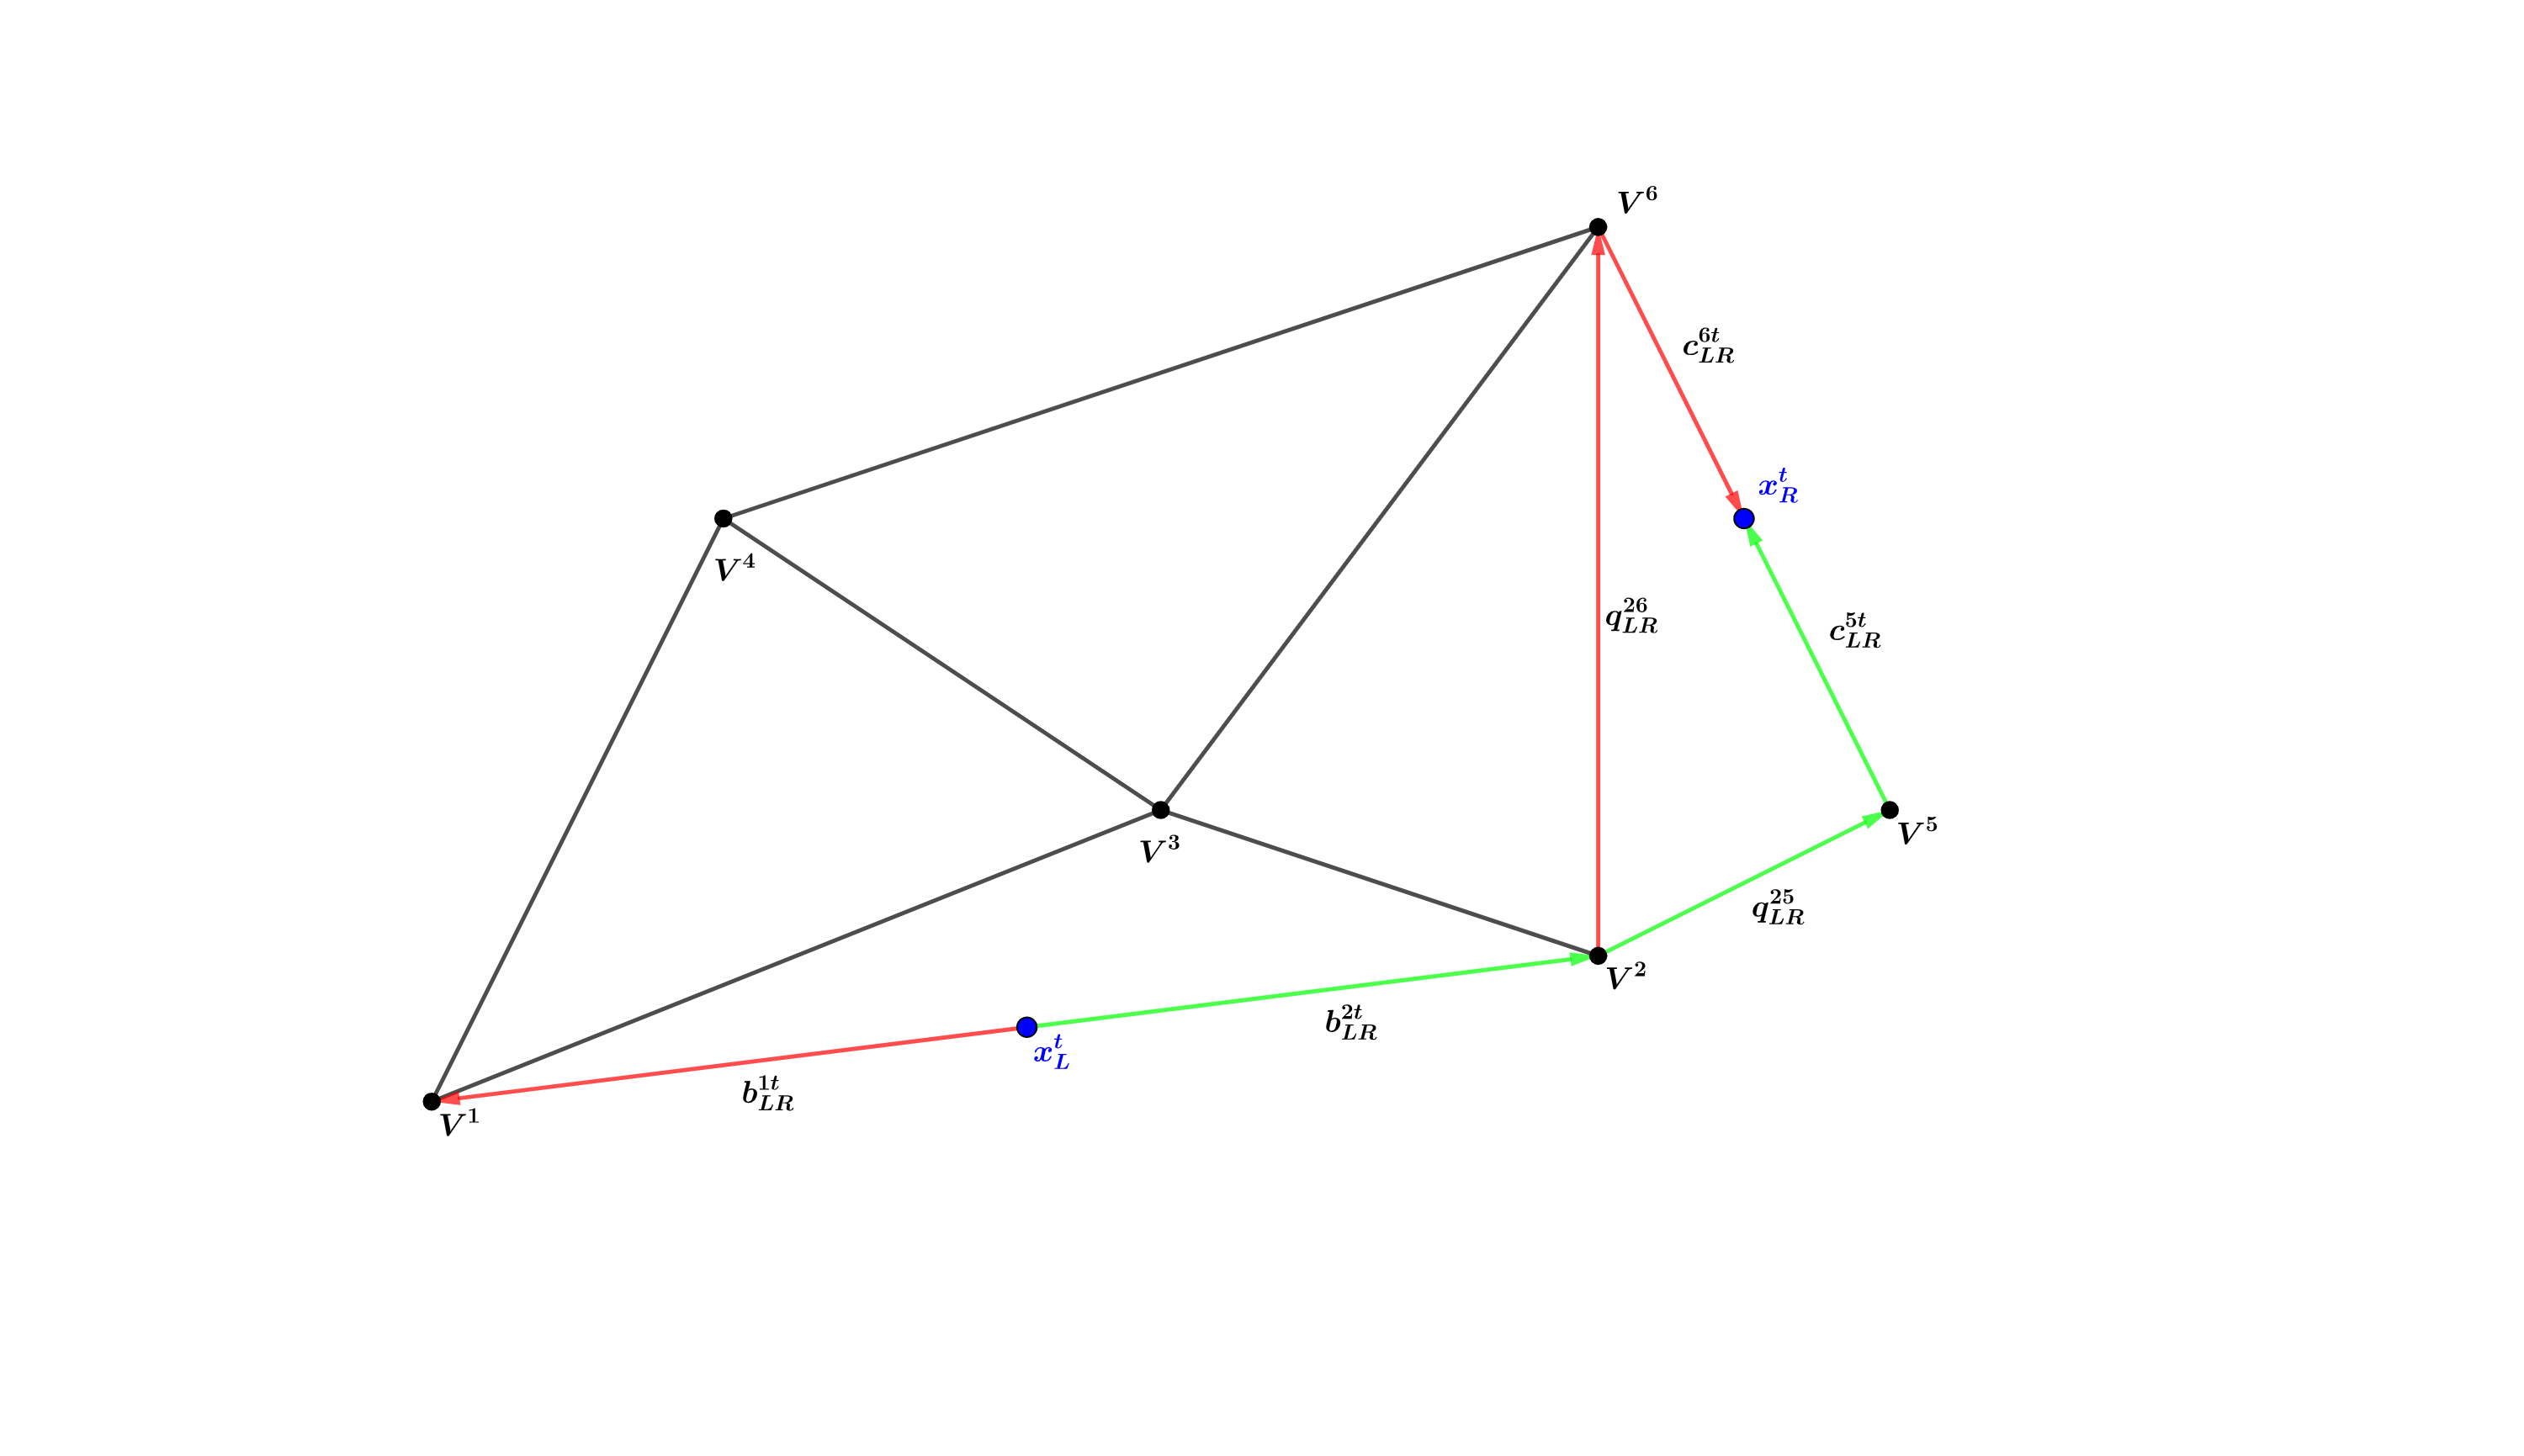
\includegraphics[width=1\linewidth]{NMDRPG.png}
             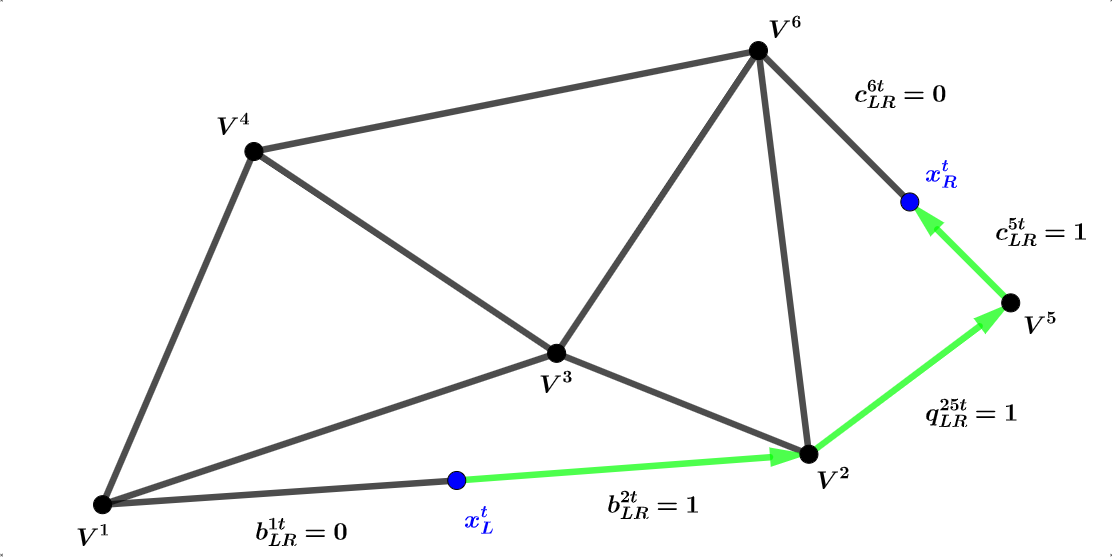
\includegraphics[width=0.45\linewidth]{NMDRPG_new.png}
             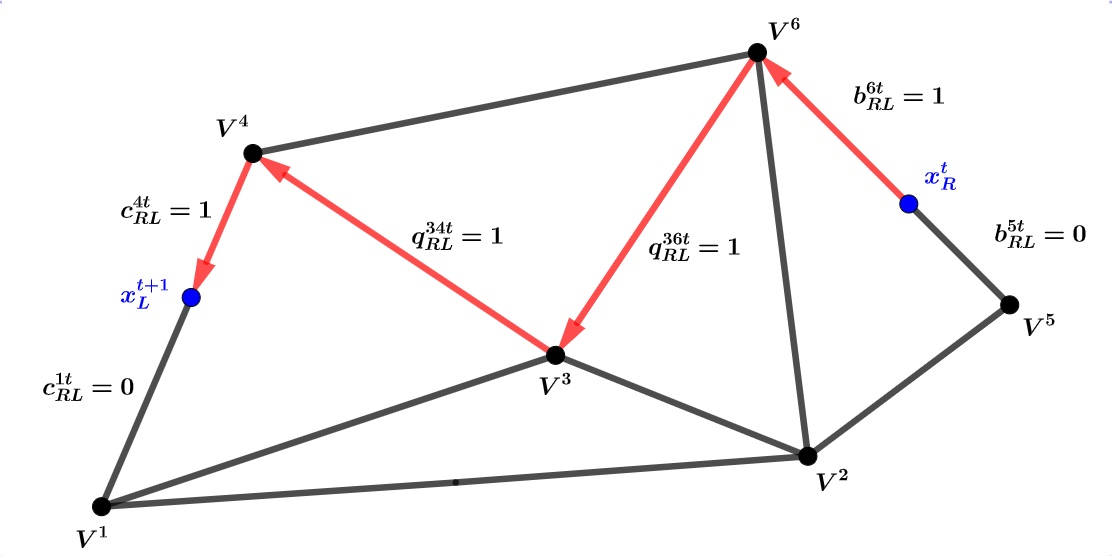
\includegraphics[width=0.45\linewidth]{NMDRPG_new2.jpg}
            \end{center}
            \caption{\LA{An example of a parameterization of a mothership route for a stage $t$. In the first picture, the mothership launches the drone at the point $x_L^t$ on the edge $\overline{V^1V^2}$, then traverses the edge $\overline{V^2V^3}$ and finally moves to $x_R^t$ on the edge $\overline{V^4V^5}$ to retrieve it. In the second one, the mothership retrieves the drone at the point $x_R^t$ on the edge $\overline{V^4V^5}$, then traverses the edge $\overline{V^3V^6}$, the edge $\overline{V^3V^4}$ and finally moves to $x_L^{t+1}$ on the edge $\overline{V^1V^4}$ to launch the drone for the next stage.}}
            \label{fig:NMDRPG}
        \end{figure}
	\end{frame}
	
	\begin{frame}{Modeling the distance inside the graph}
	\begin{small}
	With the definition one can account for the movement of the mothership at each stage $t\in T$ from a launching to a rendezvous point:\end{small}
	\begin{tiny}
	{\color{red}
    \begin{align}
        x_L^t & = \sum_{e=(i, j)\in E} \mu_{L}^{et}\left[V^i + \gamma_{L}^{et}(V^j - V^i)\right], & \quad \forall t \in T,\label{st:param1bis}\\
        x_R^t & = \sum_{e=(i, j)\in E} \mu_{R}^{et}\left[ V^i + \gamma_{R}^{et}(V^j - V^i)\right],  & \quad \forall t \in T, \label{st:param2bis}\\
      z_{LR}^{ee't} & = \mu_{L}^{et}\mu_{R}^{e't},  & \quad \forall e,e' \in E, \:\:  \forall t \in T, \label{st:prodLRbis}\\
        b_{LR}^{it} & \leq \sum_{e\in\delta(i)}\mu_{L}^{et}, \label{st:bLt1}&\qquad\forall i\in V, \:\: \forall t \in T, \\
        c_{LR}^{it} & \leq \sum_{e\in\delta(i)}\mu_{R}^{et}, \label{st:cLt1}&\qquad\forall i\in V, \:\: \forall t \in T, \\
        b_{LR}^{it} + b_{LR}^{jt} & \geq \mu_L^{et}, &\qquad \forall e=(i, j)\in E, \:\: \forall t \in T, \label{st:bLt2}\\
        c_{LR}^{it} + c_{LR}^{jt} & \geq \mu_R^{et}, &\qquad \forall e=(i, j)\in E, \:\: \forall t \in T, \label{st:cLt2}\\
        b_{LR}^{it} + \sum_{\{j:(i, j)\in E\}} q_{LR}^{jit} & = \sum_{\{j:(i, j)\in E\}} q_{LR}^{ijt} +  c_{LR}^{it}, \label{st:flow}&\qquad \forall i \in V, \:\: \forall t \in T, \\
        \sum_{e\in E} \mu_{L}^{et} & = 1, & \:\: \forall t \in T, \label{st:muLe} \\
        \sum_{e\in E} \mu_{R}^{et} & = 1, &\:\: \forall t \in T, \label{st:muRe}\\
        d_{LR}^t & = \sum_{e, e'\in E} z_{LR}^{ee't} d_{LR}^{ee't}, &\:\: \forall t \in T.  \label{st:dLRt}
    \end{align}}
    \end{tiny}
    \end{frame}
    
    \begin{frame}{Modeling the distance inside the graph}
	 We can use a set of constraints similar to those used above and the distance from $x_R^t$ to $x_L^{t+1}$ can be computed by means of the following additional constraints:
	\begin{tiny}
	{\color{red}
    \begin{align}
        z_{RL}^{ee't} & = \mu_{R}^{et}\mu_{L}^{e't+1},\label{st1:prodRL}\\
        b_{RL}^{it} & \leq \sum_{e\in\delta(i)}\mu_{R}^{et}, \label{st1:bRt1}&\qquad \forall i\in V,\:\:  \forall t \in T, \\
        c_{RL}^{it} & \leq \sum_{e\in\delta(i)}\mu_{L}^{et}, \label{st1:cRt1}&\qquad \forall e\in\delta(i),\,\forall i\in V, \:\:  \forall t \in T,\\
        b_{RL}^{it} + b_{RL}^{jt} & \geq \mu_R^{et}, &\qquad \forall e=(i, j)\in E, \:\:  \forall t \in T, \label{st1:bRt2}\\
        c_{RL}^{it} + c_{RL}^{jt} & \geq \mu_L^{et+1}, &\qquad \forall e=(i, j)\in E, \:\:  \forall t \in T, \label{st1:cRt2}\\
        b_{RL}^{it} + \sum_{\{j:(i, j)\in E\}} q_{RL}^{jit} & = \sum_{\{j:(i, j)\in E\}} q_{RL}^{ijt} +  c_{RL}^{it}, \label{st1:flow}&\qquad \forall i \in V, \:\:  \forall t \in T, \\
        \sum_{e\in E} \mu_{L}^{et} & = 1,  &\qquad \forall t \in T, \label{st1:muLe} \\
        \sum_{e\in E} \mu_{R}^{et} & = 1, &\qquad \forall t \in T, \label{st1:muRe}\\
        d_{RL}^t & = \sum_{e, e'\in E} z_{RL}^{ee't} d_{RL}^{ee't}, &\qquad \forall t \in T. \label{st1:dRLtN}
    \end{align}}
    \end{tiny}
    \end{frame}	
	
	\begin{frame}{Formulation for the NMDRPG-ST}
	
	\begin{align*}
	    \text{min}\quad &\sum_{g\in\mathcal G}\sum_{e_g\in E_g}\sum_{t\in T} (u^{e_gt}d_L^{e_gt} + v^{e_gt}d_R^{e_gt}) + \sum_{g\in\mathcal G}\sum_{e_g\in E_g} \mu^{e_g}d^{e_g} + \\
	    + & \sum_{g\in\mathcal G}\sum_{e_g,e^\prime_g\in E_g}z^{e_ge^\prime_g}d^{e_ge^\prime_g} + \sum_{t\in T} (d_{RL}^t + d_{LR}^t) \\
	    \text{s.t.}\quad & \eqref{st:DEnt}-\eqref{st:DInv}, \\
	    & \textcolor{red}{\eqref{st:param1bis}-\eqref{st1:dRLtN}}, \\
	    & \eqref{MTZ1} - \eqref{MTZ2} \text{ or } \eqref{SEC}, \\
	    & \eqref{eq:alpha-E} \text{ or } \eqref{eq:alpha-G}, \\
	    & \eqref{DCW-t}, \\
	    & \textcolor{red}{\eqref{eq:dLRNt}, \eqref{eq:dRLNt}}, \\
	    & \eqref{eq:d1}-\eqref{eq:d6}, \\
	    & \eqref{eq:O1}-\eqref{eq:D2}.
	\end{align*}
	    
	\end{frame}
	
	\begin{frame}{{\large Binary and Integer Decision Variables for the NMDRPG-MTZ}}
	\textbf{Drone tour variables}
	\begin{itemize}
	    \small
	    \item $\mu^{e_g} \in \{0,1\} \:\: \forall e_g \in E_g$ ($g \in \mathcal{G}$): equal to 1 if edge $e$ of graph $g$ (or a portion of it) is visited by the drone, and 0 otherwise.
        \item $entry^{e_g} \in \{0,1\} \:\: \forall e_g \in E_g$ ($g \in \mathcal{G}$): auxiliary binary variables for linearization.
        \item $u^{e_{g}} \in \{0,1\} \:\: \forall e_g \in E_g$ ($g \in \mathcal{G}$): equal to 1 if the drone enters in graph $g$ by $e_g$, 0 otherwise.
        \item $z^{e_{g}e^{'}_{g}} \in \{0,1\} \:\: \forall e_g, e_g' \in E_g$ ($g \in \mathcal{G}$): equal to 1 if the drone goes from $e_g$ to $e^{'}_{g}$, 0 otherwise.
        \item $v^{e_{g}} \in \{0,1\} \:\: \forall e_g \in E_g$ ($g \in \mathcal{G}$): equal to 1 if the drone exits from graph $g$ by $e_g$, 0 otherwise.
        \item $w^{gg'} \in \{0,1\} \:\:\ \forall g,g' \in \mathcal{G}$: equal to 1 if the mothership moves from $x_R^g$ to $x_L^{g^'}$, 0 otherwise.
        \item $s^{e_g} \:\: \forall e_g \in E_g$ ($g \in \mathcal{G}$): integer non negative variables representing the order of visit of edge $e$ of graph $g$.
    \end{itemize}
    \end{frame}
    
    \begin{frame}{{\large Binary and Integer Decision Variables for the NMDRPG-MTZ}}
    \textbf{Mothership tour variables inside the network}
    \small
    \begin{itemize}
        \item $\mu_{L}^{eg} \in \{0, 1\}\:\: \forall e \in E, \:\:\ \forall g \in \mathcal{G}$: equal to 1 if the launching point $x_L^g$ to visit graph $g$ is located on $e$.
        \item $\mu_{R}^{eg} \in \{0, 1\}\:\: \forall e \in E, \:\:\ \forall g \in \mathcal{G}$: equal to 1 if the rendezvous point to visit graph $g$ is located on $e$. 
        \item $z_{LR}^{ee'g} \in \{0,1\} \:\: \forall e, e' \in E, \:\:\forall g \in \mathcal{G}$: equal to 1 if the launching point $x_L^g$  to visit graph $g$ is located on $e$ and the rendezvous point $x_R^g$ is located on $e^{\prime}$.
        \item $b_{LR}^{ig} \in \{0,1\}, \:\: \forall i: e=(i,j) \in E, \:\:\ \forall g \in \mathcal G$, equal to 1 if the mothership exits from $x_L^g$ by the vertex $V^i$ of the edge $e$.
        \item $c_{LR}^{ig} \in \{0,1\}, \:\: \forall i: e=(i,j) \in E, \:\:\ \forall g \in \mathcal G$, equal to 1 if the mothership enters in $x_R^g$ by the vertex $V^i$ of the edge $e$.
        \item $q_{LR}^{eg}\geq 0, \:\:\ \forall e \in E, \:\: \forall g \in \mathcal{G}$, integer variable counting the number of times the mothership fully traverses   edge $e$ to move between the launching point $x_L^g$ on $e$ to the rendezvous point $x_R^g$ on $e'$ for graph $g$.
    \end{itemize}
    \end{frame}
    
    \begin{frame}{{\large Binary and Integer Decision Variables for the NMDRPG-MTZ}}
    \textbf{Mothership tour variables inside the network}
    \begin{itemize}
        \item $z_{RL}^{ee'gg'} \in \{0,1\} \:\: \forall e, e' \in E, \:\: \forall g, g' \in \matchal{G}$: equal to 1 if the rendezvous point $x_R^g$, for graph $g$, is located on $e$  and the launching point $x_L^{g'}$, for graph $g'$, is located on $e^{\prime}$.
        \item $b_{RL}^{ig} \in \{0,1\}, \:\: \forall i: e=(i,j) \in E, \:\:\ \forall g \in \mathcal G$, equal to 1 if the mothership exits from $x_R^g$ by the vertex $V^i$ of the edge $e$.
        \item $c_{RL}^{ig} \in \{0,1\}, \:\: \forall i: e=(i,j) \in E, \:\:\ \forall g \in \mathcal G$, equal to 1 if the mothership enters in $x_L^g$ by the vertex $V^i$ of the edge $e$.
        \item $q_{RL}^{egg'}\geq 0, \:\:\ \forall e \in E, \:\: \forall g \in \mathcal{G}$, integer variable counting the number of times the mothership fully traverses   edge $e$ to move between the rendezvous point $x_R^g$ to the launching point $x_L^{g'}$ for graph $g$.
    \end{itemize}
    \end{frame}
    
    \begin{frame}{Continuous Decision Variables for the NMDRPG-MTZ}
	\textbf{Location variables}
	\small
	\begin{itemize}
        \item $\rho^{e_g} \in [0,1]$ and $\lambda^{e_g} \in [0,1] \:\: \forall e_g \in E_g$ ($g \in \mathcal{G}$): defining the entry and exit points on edge $e_g$.
        \item $\gamma_R^{eg} \in [0,1]$ and $\gamma_{L}^{eg} \in [0,1] \:\: \forall e \in E, \:\: \forall g \in \mathcal{G}$: defining the launching and rendezvous points, associated with graph $g$, located on edge $e$ of the network $\mathcal{N}$.
        \item $\nu_\text{min}^{e_g}$ and $\nu_\text{max}^{e_g} \in [0,1] \:\: \forall e_g \in E_g$ ($g \in \mathcal{G}$): auxiliary variables for linearization.
        \item $x_L^g \:\:\ g \in \mathcal{G}$: coordinates representing the point where the mothership launches the drone to visit graph $g$.
        \item $x_R^g \:\:\ g \in \mathcal{G}$: coordinates representing the point where the mothership retrieves the drone to visit graph $g$.
        \item $R^{e_g} \:\: \forall e_g \in E_g$ ($g \in \mathcal{G}$): coordinates representing the entry point on edge $e$ of graph $g$.
        \item $L^{e_g} \:\: \forall e_g \in E_g$ ($g \in \mathcal{G}$): coordinates representing the exit point on edge $e$ of graph $g$.
    \end{itemize}
    \end{frame}
    
    \begin{frame}{Continuous Decision Variables for the NMDRPG-MTZ}
    \textbf{Distance variables}
    \begin{itemize}
        \scriptsize
        \item $d_L^{e_g} \geq 0 \:\: \forall e_g \in E_g$ ($g \in \mathcal{G}$): representing the distance travelled by the drone from the launching point
         $x_L^g$ on the mothership to the first visiting point $R^{e_g}$ on $e_g$.
        \item $d^{e_ge^\prime_g} \geq 0 \:\: \forall e_g, e^\prime_g \in E_g $ ($g \in \mathcal{G}$): representing the distance travelled by the drone from launching point $L^{e_g}$
         on $e_g$ to the rendezvous point $R^{e^\prime_g}$ on $e^\prime_g$.
        \item $d^{e_g} \geq 0 \:\: \forall e_g \in E_g$ ($g \in \mathcal{G}$): representing the distance travelled by the drone from the rendezvous point 
         $R^{e_g}$ to the launching point $L^{e_g}$ on $e_g$. 
        \item $d_R^{e_g} \geq 0 \:\: \forall e_g \in E_g$ ($g \in \mathcal{G}$): representing the distance travelled by the drone from the last visiting point 
         for graph $g$ $L^{e_g}$ to the rendezvous point $x_R^g$ on the mothership.
        \item $d_{LR}^{e e^{\prime}g} \geq 0 \:\: \forall e,\:\: e' \in E, \:\: \forall g \in \mathcal{G}$: representing the distance travelled by the mothership from the launching 
         point $x_L^g$ on $e$ and the rendezvous point $x_R^g$ on $e'$ to visit graph $g$.
        \item $d_{RL}^{e e^{\prime}g g'} \geq 0 \:\: \forall e,\:\:\ e' \in E \:\: \forall g,\:\: g' \in \mathcal{G}$: representing the distance travelled by the mothership from the 
         rendezvous point $x_R^g$, for graph $g$, on $e$ to the launching point $x_L^{g'}$, for graph $g'$, on $e'$.
        \item  $d^{g}_{LR} \geq 0 \:\: \forall g \in \mathcal{G}$: representing the total distance
        travelled by the mothership between the launching point 
         $x_L^g$ and the rendezvous point $x_R^g$ to visit graph $g$.
        \item $d^{gg'}_{RL}\geq 0 \:\: \forall g, \:\: g' \in \mathcal{G}$, representing the total distance travelled by the mothership between the rendezvous
         point $x_R^g$, for graph $g$, and the launching point $x_L^{g'}$, for graph $g'$.
    \end{itemize}
	\end{frame}
	\begin{frame}{Modeling the distance inside the graph}
        In this case, we observe that the distance between launching and rendezvous points in two edges $e=(i,j),\, e'=(i',j')\in E$, not necessarily distinct,  of the graph can be represented as:
        \begin{tiny}
        \begin{equation}\tag{$d^{g\mathcal N}_{LR}$}\label{eq:dLRg}
        d_{LR}^{ee'g} = \left\{\begin{matrix}
        |\gamma_{L}^{eg} - \gamma_{R}^{eg}|\mathcal L(e), & \text{if } e = e',\\
        \left[b_{LR}^{ig}\gamma_{L}^{eg} + b_{LR}^{jg}(1 - \gamma_{L}^{eg})\right]\mathcal L(e) + \displaystyle \sum_{e''\in \mathcal N}q_{LR}^{e''g}\mathcal L(e'') + \left[c_{LR}^{i'g}\gamma_{R}^{e'g} + c_{LR}^{j'g}(1 - \gamma_{R}^{e'g})\right]\mathcal{L}(e'), & \text{if } e \neq e',
        \end{matrix}\right.
        \end{equation}
        \end{tiny}
    	
        Similarly, the distance covered by the mothership along the path on the network $\mathcal{N}$, from the rendezvous point $x_R^g\in e$, after the visit to $g\in \mathcal{G}$ to the next launching point $x_L^{g'}\in e'$ (to go to the graph $g'\in \mathcal{G}$), can be modeled using the following definition of distance:
        
        \begin{tiny}
            \begin{equation}\tag{$d^{g\mathcal N}_{RL}$}\label{eq:dRLg}
            d_{RL}^{ee'gg'} = \left\{\begin{matrix}
            |\gamma_{R}^{eg} - \gamma_{L}^{eg'}|\mathcal L(e), & \text{if } e = e',\\
            \left[b_{RL}^{ig}\gamma_{R}^{eg} + b_{RL}^{jg}(1 - \gamma_{R}^{eg})\right]\mathcal L(e) + \displaystyle \sum_{e''\in \mathcal N}q_{RL}^{e''gg'}\mathcal L(e'') + \left[c_{RL}^{i'g'}\gamma_{L}^{e'g'} + c_{RL}^{j'g'}(1 - \gamma_{L}^{e'g'})\right]\mathcal L(e'), & \text{if } e \neq e'.
            \end{matrix}\right.
            \end{equation}
        \end{tiny}
	\end{frame}
	
	\begin{frame}{Modeling the distance inside the graph}
	    
        \begin{tiny}
        	All the above arguments give the necessary elements to account for the movement of the mothership on the network $\mathcal{N}=(V,E)$ from $x_L^g$ to $x_R^g$:
        \begin{align}
            x_L^g & = \sum_{e=(i, j)\in E} \mu_{L}^{eg}\left[V^i + \gamma_{L}^{eg}(V^j - V^i)\right], &\qquad \forall g \in \mathcal{G}, \label{g:param1bisg}\\
            x_R^g & = \sum_{e=(i, j)\in E} \mu_{R}^{eg}\left[ V^i + \gamma_{R}^{eg}(V^j - V^i)\right], &\qquad \forall g \in \mathcal{G}, \label{g:param2bisg}\\
            z_{LR}^{ee'g} & = \mu_{L}^{eg}\mu_{R}^{e'g}, &\qquad \forall e,e' \in E, \:\: \forall g \in \mathcal{G},\label{g:prodLR}\\
            b_{LR}^{ig} & \leq \sum_{e\in\delta(i)} \mu_{L}^{eg}, \label{g:bLt1}&\qquad \forall i\in V, \quad \forall g \in \mathcal{G}, \\
            c_{LR}^{ig} & \leq \sum_{e\in\delta(i)} \mu_{R}^{eg}, \label{g:cLt1}&\qquad \forall i\in V, \quad \forall g \in \mathcal{G},\\
            b_{LR}^{ig} + b_{LR}^{jg} & \geq \mu_L^{eg}, &\qquad \forall e=(i, j)\in E, \quad \forall g \in \mathcal{G},\label{g:bLt2}\\
            c_{LR}^{ig} + c_{LR}^{jg} & \geq \mu_R^{eg}, &\qquad \forall e=(i, j)\in E, \quad \forall g \in \mathcal{G}, \label{g:cLt2}\\
            b_{LR}^{ig} + \sum_{\{j:(i, j)\in E\}} q_{LR}^{jig} & = \sum_{\{j:(i, j)\in E\}} q_{LR}^{ijg} +  c_{LR}^{ig}, \label{g:flow}&\qquad \forall i \in V, \quad \forall g \in \mathcal{G},\\
            \sum_{e\in E} \mu_{L}^{eg} & = 1, &\qquad \forall g \in \mathcal{G}, \label{g:muLe} \\
            \sum_{e\in E} \mu_{R}^{eg} & = 1, &\qquad \forall g \in \mathcal{G}, \label{g:muRe}\\
            d_{LR}^g & = \sum_{e, e'\in E} z_{LR}^{ee'g} d_{LR}^{ee'g}. &\qquad \forall g \in \mathcal{G}. \label{g:dLRgN}
        \end{align}
        \end{tiny}
	    
	\end{frame}
	
	\begin{frame}{Modeling the distance inside the graph}
        We can use a set of constraints similar to those used above and the distance from $x_R^g$ to $x_L^{g'}$ can be computed by means of the following additional constraints:
        \begin{tiny}
        \begin{align}
            z_{RL}^{ee'gg'} & = \mu_{R}^{eg}\mu_L^{e'g'}, &\qquad \forall e,e' \in E,\:\:\ \forall g,g' \in \mathcal{G},\label{prodRLggN}\\
            b_{RL}^{ig} & \leq \sum_{e\in\delta(i)}\mu_{R}^{eg}, \label{bRt1}&\qquad \forall i\in V, \:\: \forall g \in \mathcal{G}, \\
            c_{RL}^{ig} & \leq \sum_{e\in\delta(i)}\mu_{L}^{eg}, \label{cRt1}&\qquad \forall i\in V, \:\: \forall g \in \mathcal{G},\\
            b_{RL}^{ig} + b_{RL}^{jg} & \geq \mu_R^{eg}, &\qquad \forall e=(i, j)\in E, \:\: \forall g \in \mathcal{G},\label{bRt2}\\
            c_{RL}^{ig} + c_{RL}^{jg} & \geq \mu_L^{eg}, &\qquad \forall e=(i, j)\in E, \:\: \forall g \in \mathcal{G},\label{cRt2}\\
            b_{RL}^{ig} + \sum_{\{j:(i, j)\in E\}} q_{RL}^{jigg'} & = \sum_{\{j:(i, j)\in E\}} q_{RL}^{ijgg'} +  c_{RL}^{ig'}, \label{flow}&\qquad \forall i \in V, \:\: \forall g \in \mathcal{G},\\
            d_{RL}^{gg'} & = \sum_{e, e'} z_{RL}^{ee'gg'} d_{RL}^{ee'gg'}, & \qquad\:\: \forall g,g' \in \mathcal{G}.\label{dRLt}
        \end{align}
        \end{tiny}
    \end{frame}
    
    \begin{frame}{Formulation for the NMDRPG-MTZ}
	\small
	\begin{align*}
	    \text{min}\quad &\sum_{g\in\mathcal G}\sum_{e_g\in E_g} (u^{e_g}d_L^{e_g} + v^{e_g}d_R^{e_g}) + \sum_{g\in\mathcal G}\sum_{e_g\in E_g} \mu^{e_g} d^{e_g} + \\
	    + & \sum_{g\in\mathcal G}\sum_{e_g,e^\prime_g\in E_g}z^{e_ge^\prime_g}d^{e_ge^\prime_g} + \sum_{g\in\mathcal G} d_{LR}^g + \sum_{g,g'\in \mathcal G}d_{RL}^{gg'}w^{gg'} \\
	    \text{s.t.}\quad & \eqref{DEnt2}-\eqref{TEnt}, \\
	    & \eqref{g:param1bisg}-\eqref{dRLt}, \\
	    & \eqref{MTZ1} - \eqref{MTZ2} \text{ or } \eqref{SEC}, \\
	    & \eqref{MTZ3} - \eqref{MTZ6}, \\
	    & \eqref{eq:alpha-E} \text{ or } \eqref{eq:alpha-G}, \\
	    & \eqref{DCW-g}, \\
	    & \eqref{eq:dLRg}, \eqref{eq:dRLg}, \\
	    & \eqref{eq:d1g}-\eqref{eq:d6g}, \\
	    & \eqref{eq:O1}-\eqref{eq:D2}.
	\end{align*}
	    
	\end{frame}
    
	\begin{frame}{Example}
    	\begin{figure}
    	\centering
		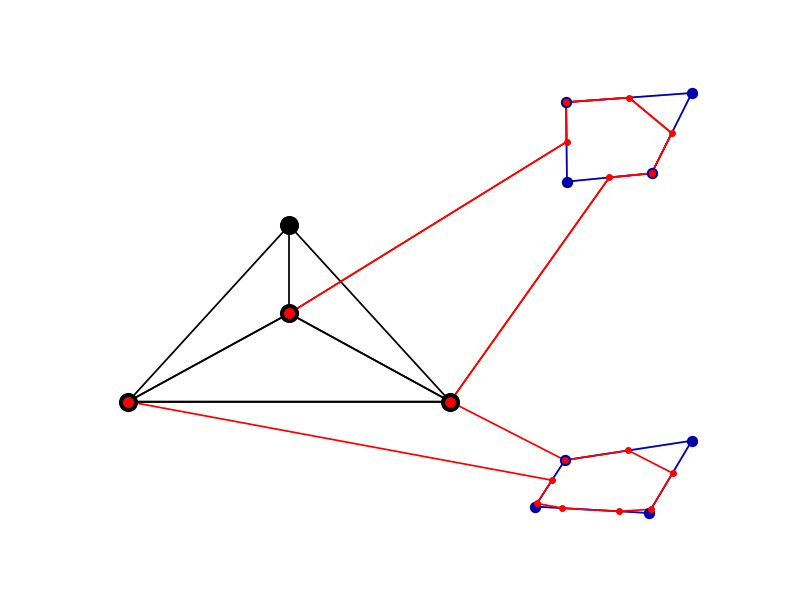
\includegraphics[width=0.6\linewidth]{NDMTZ}
		\caption{NMDRPG-MTZ example for a drone that visits the 50\% of each edge}
		\end{figure}
	\end{frame}
	
	\begin{frame}{Matheuristic for the MDRPG}
	   \textbf{Pseudo-code of this algorithm:}
	   \begin{itemize} 
            \item[STEP 1] (Centroids of the graphs)\\
            - Let $orig$ be the origin/destination of the mothership tour \\ %(orange point with label $0$ in Figure \ref{fig:example} [a]).\\
            For each graph $g \in \mathcal G$:\\
            - identify its centroid $c_g$ and consider its neighborhood defined as the circle $\rho(c_g,2)$ centered at $c_g$ and with radius 2 %(red points in Figure \ref{fig:example} [a]).
            \item[STEP 2] (Order of visit of the graphs)
            Determine an order of visit for the graphs in $\mathcal{G}$ by solving the XPPN of the mothership over the set of the neighborhoods associated with the centroids of those graphs %(blue tour 0, 1, 2, 3, 4, 0 in Figure  \ref{fig:example} [a]).\\
        \end{itemize}
    \end{frame}
    
    \begin{frame}{Matheuristic for the MDRPG}
    \textbf{Pseudo-code of this algorithm:}
    \begin{itemize}
        \small
            \item[STEP 3] (Determining the location of launching/rendezvous points)
            Let $\bar{w}_{gg^{'}}, \: \forall g,g^{'} \in \mathcal G$ be the optimal values of the variables $w_{gg^{'}}$ generated by STEP 2.\\
            Following this order of visit, set the launching point for the first graph as the depot, then solve the resulting (MDRPG) limited to the first graph.\\
            Repeat the same procedure for the remaining graphs to be visited, by solving \AMD\xspace on one single graph each time, by fixing as launching point of the current graph the rendezvous point of the previous graph.
            
            \item [STEP 4] (Solution update) 
            Let $\bar{z}$ be the solution obtained by STEP 3, consisting of the tour of the drone on each target,  %(Figure \ref{fig:example} [b])
            and let $\bar{x}_{L}^{g}$, $\bar{x}_{R}^{g} \:\: \forall g \in \mathcal G$ be the associated launching/rendezvous points %(green and blue points in Figure \ref{fig:example} [b]).\\
            Solve the model (MDRPG) with these launching/rendezvous points but leaving free the $w_{gg^{'}} \:\:\ \forall g,g^{'} \in \mathcal G$ variables and providing to the solver $\bar{z}$ as initial partial solution.
            \item [STEP 5]
            Let $\hat{z}$ be the updated solution obtained by STEP 4 %(see Figure \ref{fig:example} [b] for this illustrative example) 
            and $\hat{w}_{gg^{'}}$ the associated order of visit of the graphs.\\
            If the $\hat{w}_{gg^{'}} \neq \bar{w}_{gg^{'}}$ repeat from STEP 3, otherwise stop.
            \end{itemize}
	\end{frame}

    \begin{frame}{Example of the Matheuristic}	
		\begin{figure}%
    		\hspace{-2.5cm}
        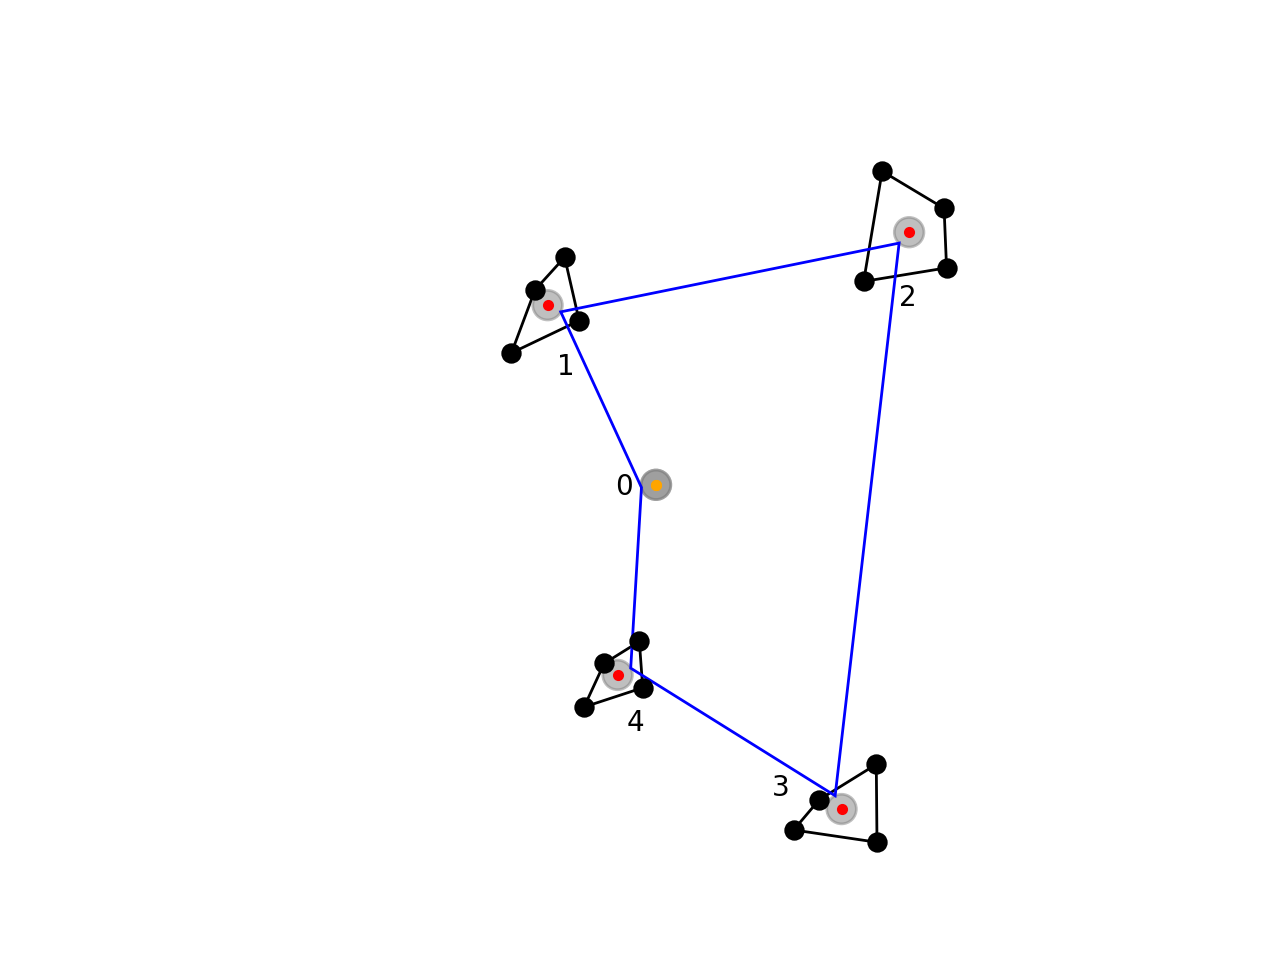
\includegraphics[width=7cm]{step0}\hspace{-1.5cm}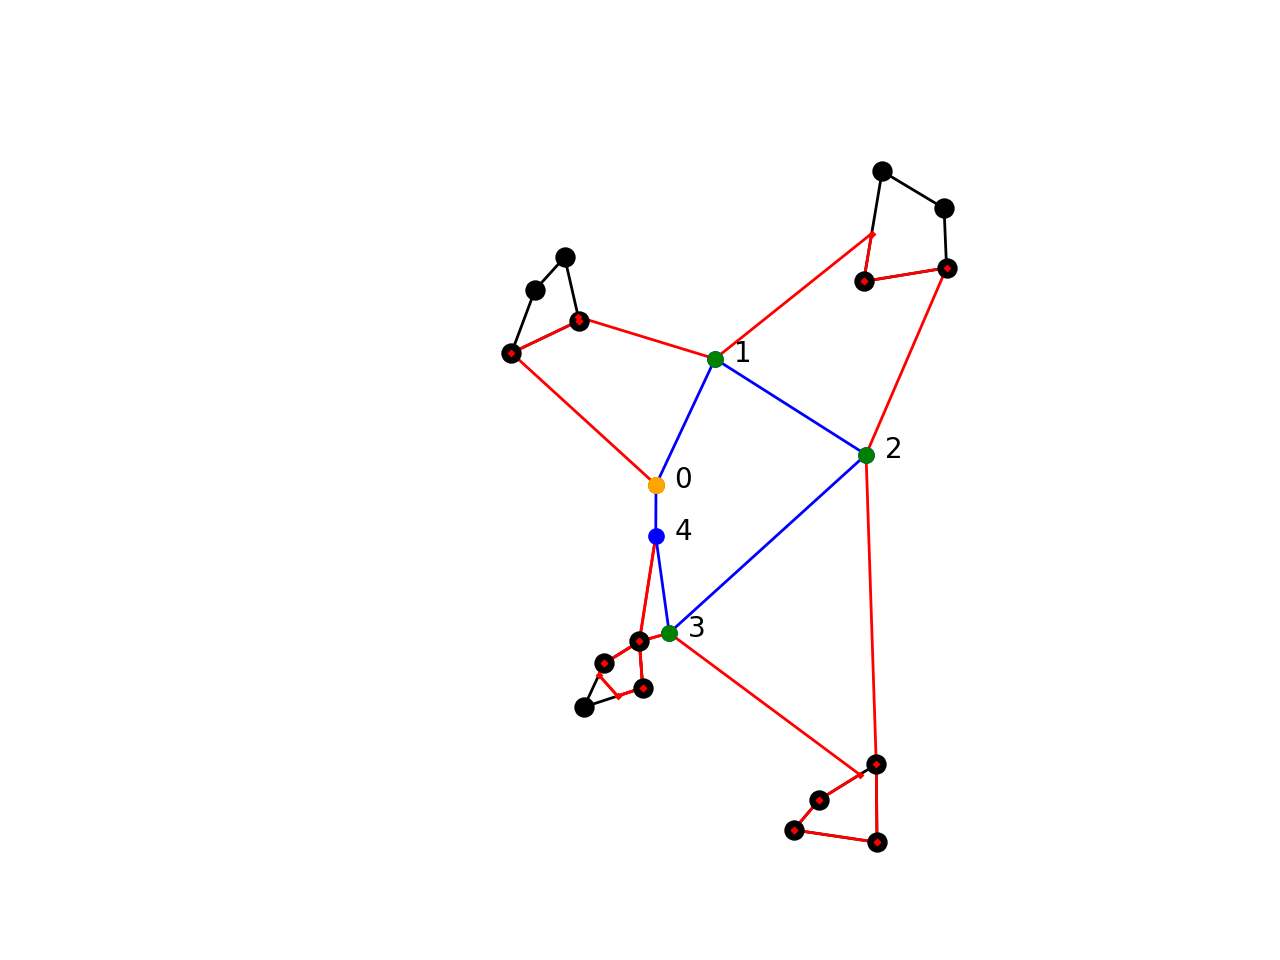
\includegraphics[width=7cm]{step1}%
        \caption{Illustrative Example}%
        \label{fig:example}%
    	\end{figure}
    \end{frame}
    
    \begin{frame}{Computational Experiments: Data Generation}
        We consider two typology of planar graphs:
        \begin{itemize}
            \item Grid graphs
            \item Delaunay triangulation (computed by using the Python class scipy.spatial.Delaunay)
        \end{itemize}
    \end{frame}
    
    \begin{frame}{Computational Experiments: Grid Generation}
    To simulate graphs that are similar to the one found in a road network, we design grid graphs following these steps:
    \begin{enumerate}
        \item We consider a square of side 100 units that we divide in subsquares of side 5 and we randomly select among them the locations for each graph.
        \item Each subsquare of side 5 selected is further partitioned in subsquares of side $\frac{5}{n}$ where $n$ is the cardinality of the set of nodes of the graph to build.
        \item Two opposite corner subsquares are considered and one point inside each of them is randomly selected.
        \item A grid of $n$ points is identified by locating $\frac{n}{m}$ equally spaced points on the two sides square rectangle whose diagonal joins these two points is built, where $m$ is randomly selected in the set of divisors of the number of points of the graph.
    \end{enumerate}
        
    \end{frame}
	
	\begin{frame}{Computational Experiments: Grid Generation}
    To simulate graphs that are similar to the one found in a road network, we design grid graphs following these steps:
    \begin{enumerate}
        \setcounter{enumi}{4}
        \item The links of the graphs connect each point to its adjacent ones lying on the same side and with the one located on the opposite side of the square.
        \item Let $width_x$ and $width_y$ be the lengths of these edges. In order to perturb the coordinates of these points, we randomly add a value, ranging between $-\frac{width_x}{3}$ and $\frac{width_x}{3}$ to the $x$ coordinate and between $-\frac{width_y}{3}$ and $\frac{width_y}{3}$ to the $y$ coordinate, always imposing that the perturbed point still belongs to the square.
        \item The resulting grid graph is obtained connecting the same pairs of points but with perturbed coordinates.
    \end{enumerate}
        
    \end{frame}
	
	\begin{frame}{Computational Experiments: Grid Generation}
        \begin{figure}[h!]
        \begin{center}
         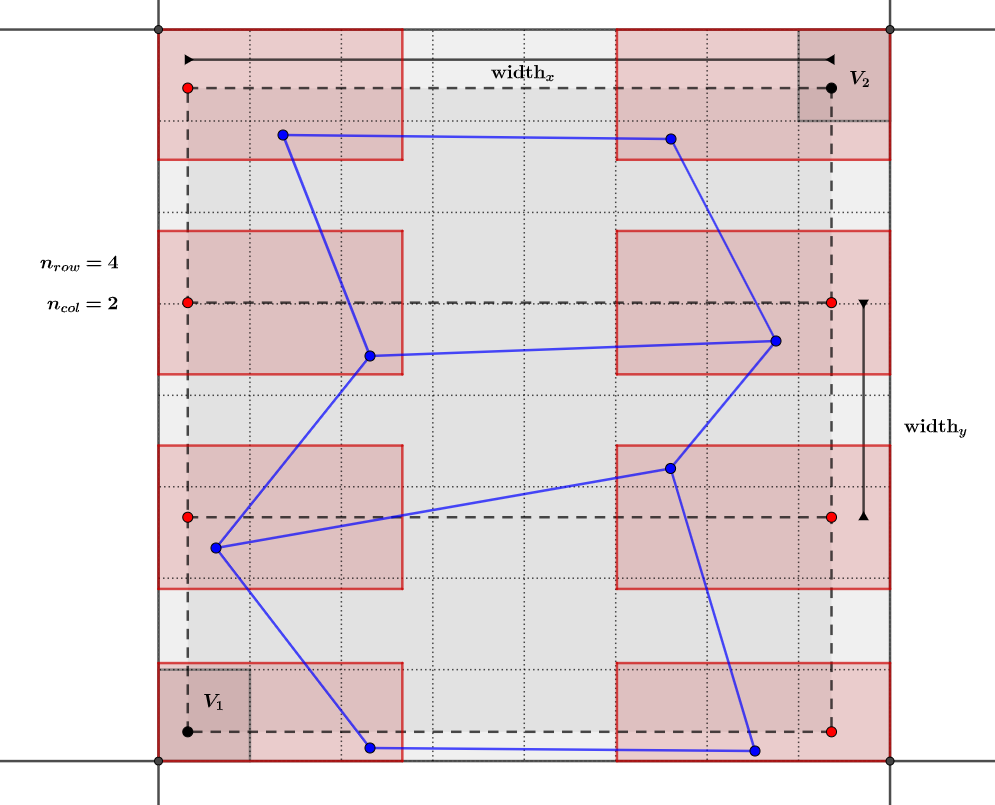
\includegraphics[width=0.6\linewidth]{Grid_generation_2.png}
        \end{center}
        \caption{Example of generation of a grid graph}
        \label{fig:fig1}
        \end{figure}
 
	\end{frame}
	
	\begin{frame}{Experiment 1: Comparing Gurobi and Cplex}
	    We generate five instances with a number $|\mathcal G|= 10$ of target graphs:
	    \begin{itemize}
	        \item 3 graphs with 4 nodes, 3 graphs with 6 nodes, 3 graphs with 8 nodes and 1 graph with 10 nodes.
	        \item $v_D= 2v_M$.
	        \item $80\%$ of each target must be visited by the drone.
	    \end{itemize}
	    
	    The experiment consists on:
	    \begin{itemize}
	        \item Running the three formulations proposed for the (AMDRPG): Stages, MTZ and SEC.
	        \item Using two commercial solvers, Cplex 12.8 and Gurobi 9.03.
	        \item Time Limit: 1 hour.
	    \end{itemize}
	\end{frame}
	
	\begin{frame}{Experiment 1: Results}
		\renewcommand{\arraystretch}{0.7}
        \begin{table}[!h]
        \caption{Comparison between formulations for grid instances}
        \centering
        \footnotesize
        \begin{tabular}{c | c c | c c | c c}
        \hline\hline
        \textbf{Gap \%} & \multicolumn{2}{c}{Average} &  \multicolumn{2}{c}{Min} &  \multicolumn{2}{c}{Max} \\
         % \hline
        \textbf{Solver} &Cplex &Gurobi &Cplex &Gurobi  &Cplex &Gurobi \\
        \hline
        \textbf{Formulation} & & & & & &\\
        Stages & 0,87 &	0,87 &	0,85 &	0,84 &	0,88 &	0,88\\
        MTZ	 & 0,66 &	0,62 &	0,59 &	0,58 &	0,72 &	0,65\\
        SEC	& 0,65 &	0,61 &	0,59 &	0,57 &	0,70 &	0,64\\
            \hline
        \end{tabular}
        \label{table:tab1}
        \end{table}
        
        \renewcommand{\arraystretch}{0.7}
        \begin{table}[!h]
        \caption{Comparison between formulations for Delauney instances}
        \centering
        \footnotesize
        \begin{tabular}{c | c c | c c | c c}
        \hline\hline
        \textbf{Gap \%} & \multicolumn{2}{c}{Average} &  \multicolumn{2}{c}{Min} &  \multicolumn{2}{c}{Max} \\
         % \hline
        \textbf{Solver} &Cplex &Gurobi &Cplex &Gurobi  &Cplex &Gurobi \\
        \hline
        \textbf{Formulation} & & & & & &\\
        Stages &	0,91 &	0,91 &	0,90 &	0,89 &	0,93 &	0,93\\
        MTZ	& 0,78 &	0,74 &	0,74 &	0,70 &	0,82 &	0,79\\
        SEC	& 0,77 &	0,75 &	0,73 &	0,69 &	0,82 &	0,81\\
            \hline
        \end{tabular}
        \label{table:tab2}
        \end{table}
	    
	\end{frame}
	
	\begin{frame}{Experiment 2: Testing the performance of the Matheuristic}
	
    We generate five instances for each number $|\mathcal G|\in\{5, 10, 15, 20\}$ of target graphs:
    \begin{itemize}
        \item The same percentage of graphs ($20\%$) has respectively 4, 6, 8, 10 and 12 nodes.
        \item $v_D= 3v_M$.
        \item $\alpha^g$ and $\alpha^{e_g}$ randomly generated in $[0, 1]$.
    \end{itemize}
    
    The experiment consists on:
    \begin{itemize}
        \item Running the MTZ formulation for (AMDRPG) with and without initial solution provided by the matheuristic.
        \item Using Gurobi 9.03.
        \item Time Limit: 2 hour.
    \end{itemize}
	    
	\end{frame}
	
	\begin{frame}{Experiment 2: Results}
    \renewcommand{\arraystretch}{0.7}
    \begin{table}[!h]
    \caption{Comparison between exact resolution with and without initialization}
    \centering
    \footnotesize
    \begin{tabular}{c c | c c c | c c c}
    \hline
     &  & \multicolumn{3}{c}{\textbf{Grid}} &  \multicolumn{3}{c}{\textbf{Delauney}} \\
    \hline
     List &  $\%$  & $\%$ Gap (i) & Time$\_$h & $\%$ Gap (wi)  & $\%$ Gap (i) & Time$\_$h &  $\%$ Gap (wi)\\
    \hline
    \multirow{}{}{0} & e & 0.72 & 105.12 & 0.73 & 0.78 & 154.92 & 0.74\\
    & g & 0.55 & 58.92 & 0.54 & 0.62 & 92.64 & 0.67\\
    \hline
    \multirow{}{}{1} & e & 0.76 & 241.99 & 0.76 & 0.80 & 314.69 & 0.79\\
    & g & 0.71 & 182.61 & 0.70 & 0.74 & 353.04 & 0.75\\
    \hline
    \multirow{}{}{2} & e & 0.76 & 367.69 & 0.76 & 0.80 & 447.61 & 0.80 \\
    & g & 0.71 & 326.49 & 0.72 & 0.76 & 429.16 & 0.76\\
    \hline
    \multirow{}{}{3} & e & 0.75 & 481.68 & 0.74 & 0.80 & 514.98 & 0.76^*\\
    & g & 0.71 & 492.27 & 0.70 & 0.77 & 582.90 & 0.77\\
        \hline
    \end{tabular}
    \label{table:tab4}
    \end{table}
	\end{frame}
	
	\begin{frame}
	    \begin{figure}
	        \centering
            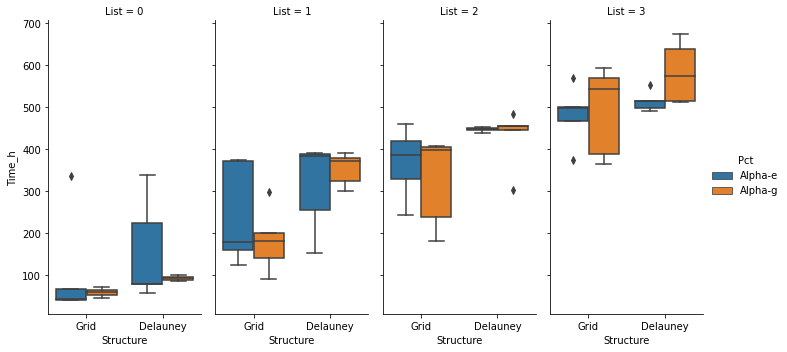
\includegraphics[width=1\linewidth]{time_h.png}
            \caption{Matheuristic running time}
            \label{fig:1}
	    \end{figure}
	\end{frame}
	\begin{frame}
	    \begin{figure}
    	    \centering
            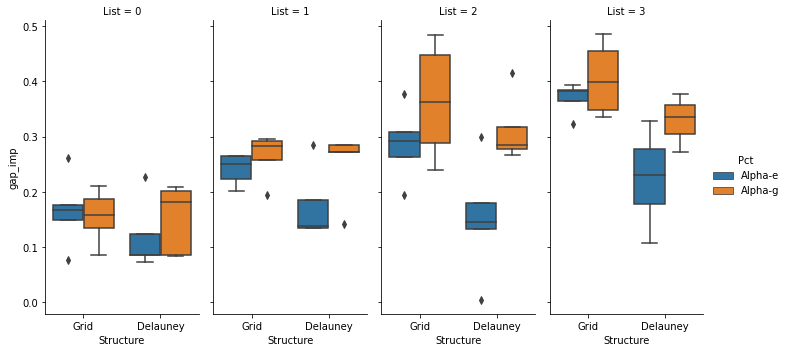
\includegraphics[width=1\linewidth]{improved_gap.png}
            \caption{Matheuristic improved gap}
	    \end{figure}
	\end{frame}
	\begin{frame}
	    \begin{figure}
            \centering
            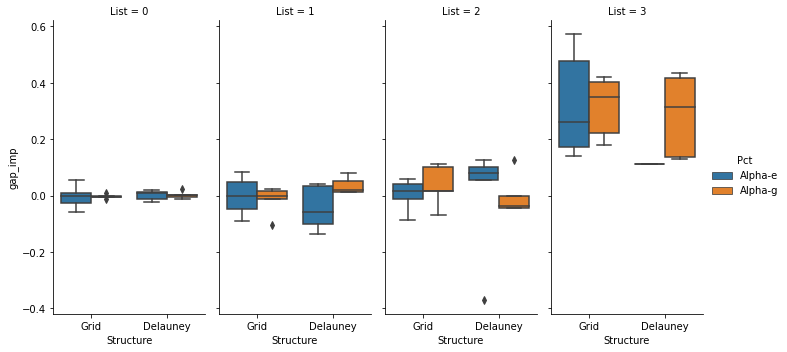
\includegraphics[width=1\linewidth]{differencewithwithout.png}
            \caption{Improved gap of MTZ formulation with and without initialization}
            \label{fig:3}
        \end{figure}
	\end{frame}
	
	
	\begin{frame}{Experiment 3: Solving the NMDRPG}
	    \begin{scriptsize}
        We generate five instances for each number $|\mathcal G|\in\{5, 10\}$ of target graphs. For each instance:
        \begin{itemize}
            \item The same percentage of graphs ($20\%$) has respectively 4, 6, 8, 10 and 12 nodes.
            \item $v_D= 3v_M$.
            \item $\alpha^g$ and $\alpha^{e_g}$ randomly generated in $[0, 1]$.
            \item \textcolor{red}{Three different network structures are considered:}
                {\color{red}
                \begin{scriptsize}
                \begin{itemize}
                    \item Graph of 6 nodes with a tree structure with origin of the path of the base vehicle different from the destination.
                    \item Complete graph of 4 vertices with origin of the path of the base vehicle different from the destination.
                    \item Star graphs of 7 nodes representing the mothership network, where the origin coincides with the destination and it is located at the centre of the star.
                \end{itemize}
                \end{scriptsize}}
        \end{itemize}
        
        The experiment consists on:
        \begin{itemize}
            \item Running the MTZ and Stages formulation for (NMDRPG) with and without initial solution provided by the matheuristic.
            \item Using Gurobi 9.03.
            \item Time Limit: 2 hour.
        \end{itemize}
	    
	\end{scriptsize} 
	\end{frame}
	
	\begin{frame}{Experiment 3: Network Structures}
	    \begin{figure}
	        \centering
	        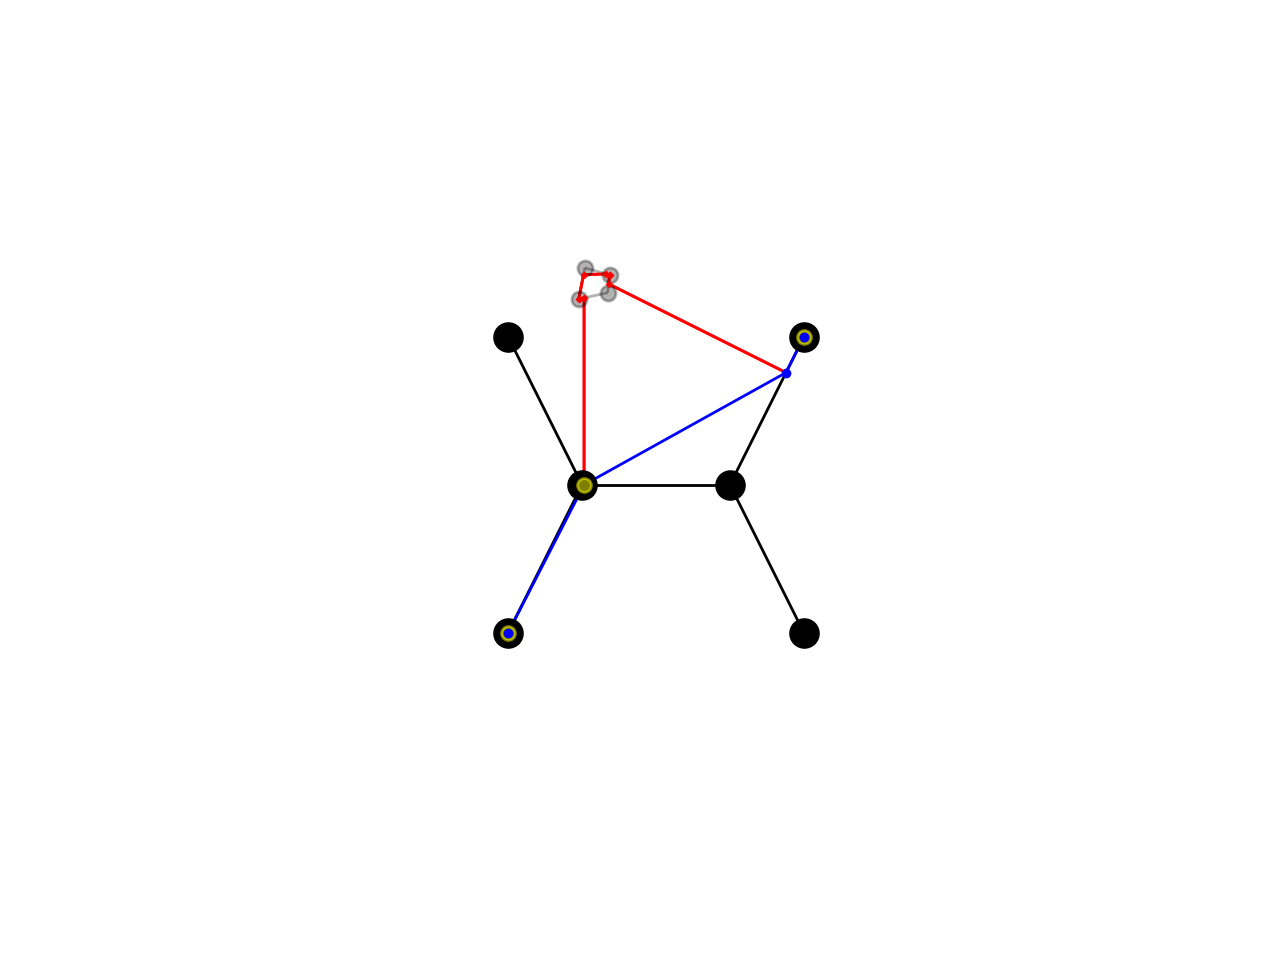
\includegraphics[width=0.33\linewidth]{NDMTZ-grid-mode1.png}
	        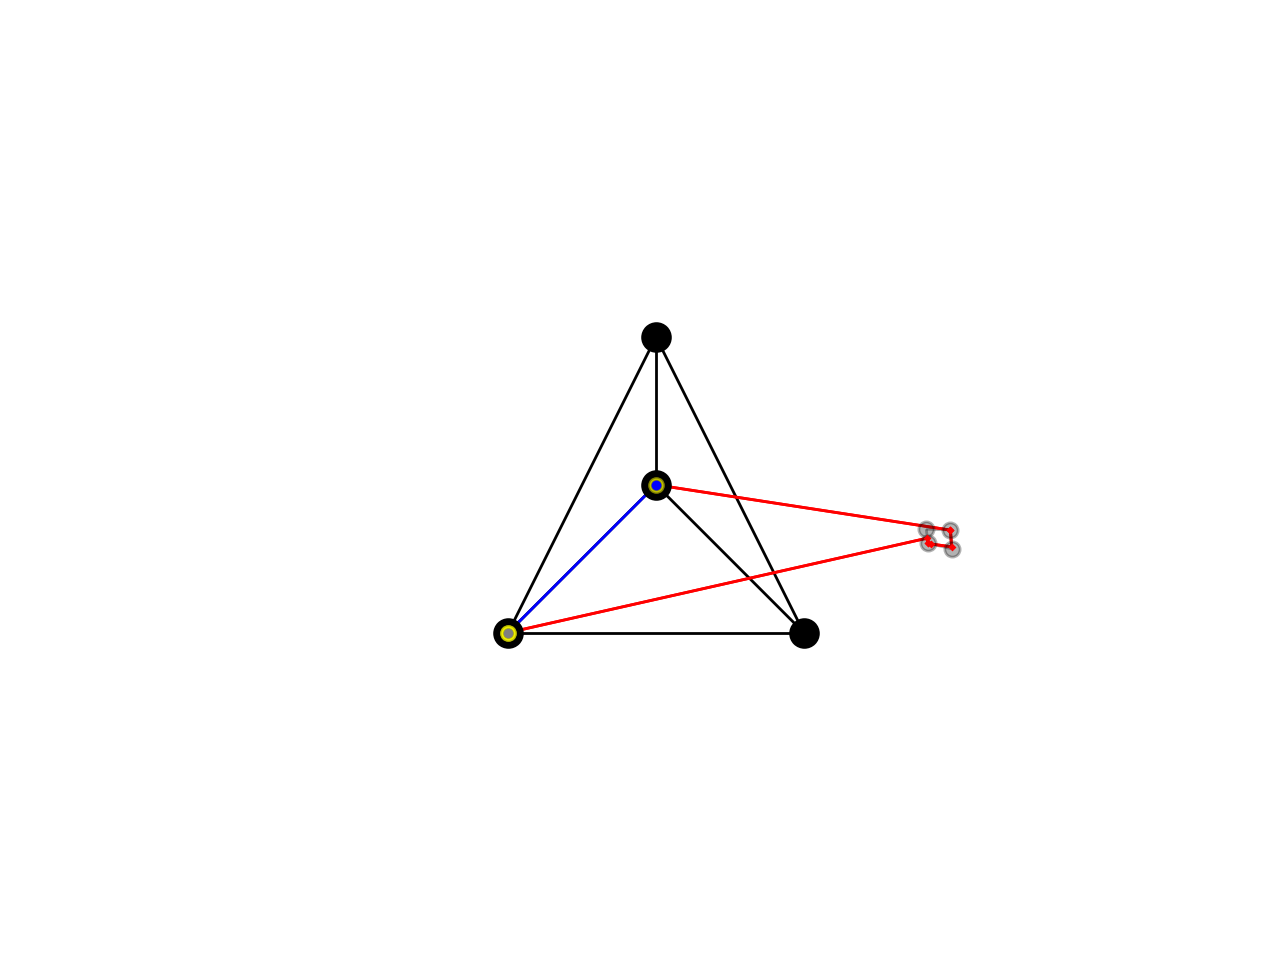
\includegraphics[width=0.33\linewidth]{NDMTZ-grid-mode2.png}
	        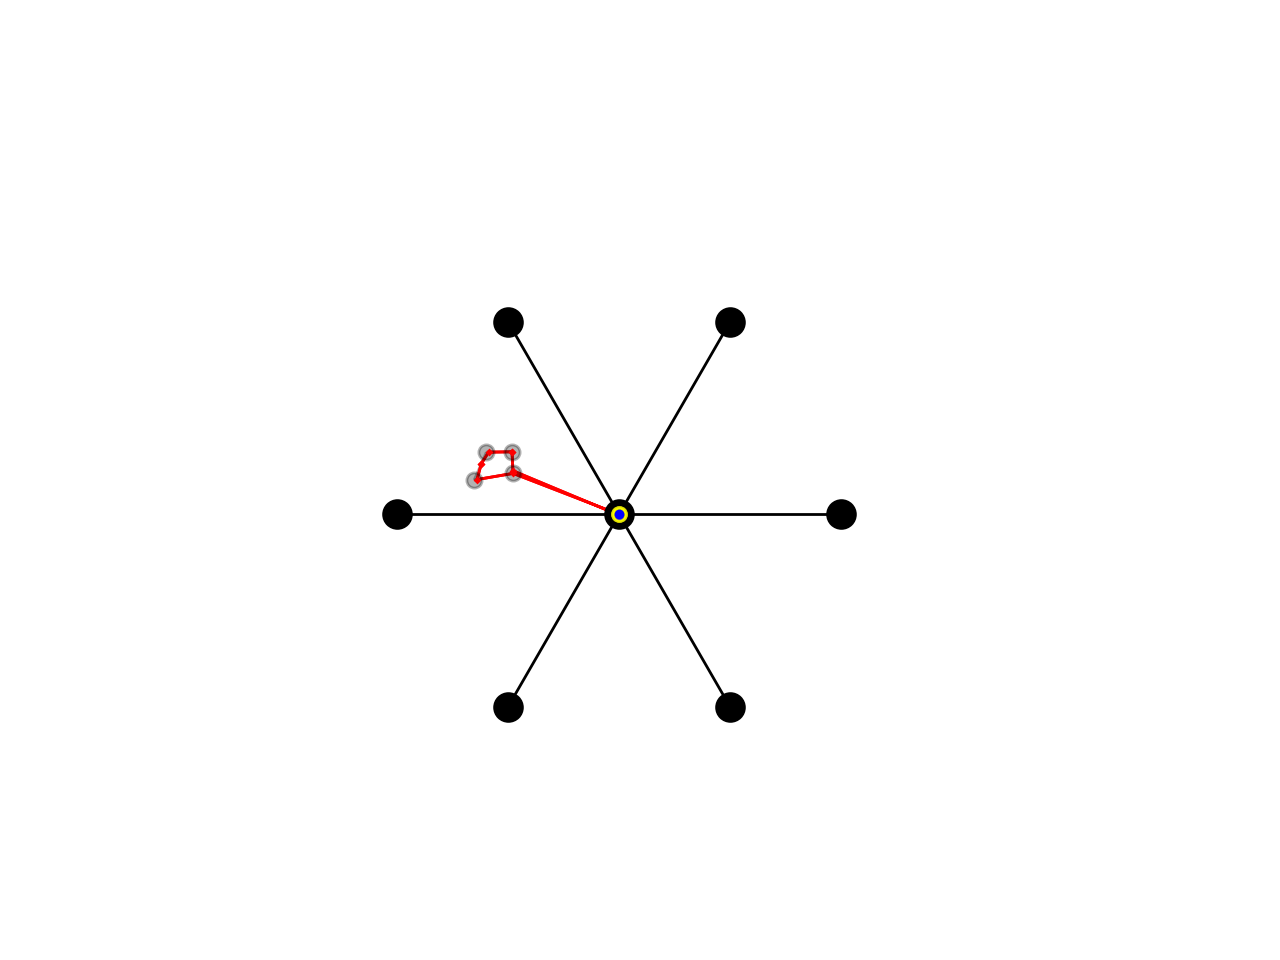
\includegraphics[width=0.33\linewidth]{NDMTZ-grid-mode3.png}
	        \caption{Network Structures}
	    \end{figure}
	\end{frame}
	
	\begin{frame}{Experiment 3: Results}
	    \begin{table}[!h]
        \caption{Comparison between formulations of the (NMDRPG)}
        \centering
        \footnotesize
        \begin{tabular}{c c | c c | c c | c c}
        \hline
         & Net Struct  & \multicolumn{2}{c}{1} &  \multicolumn{2}{c}{2}  & \multicolumn{2}{c}{3}\\
        \hline
        List & $\%$ &  Stages  & MTZ & Stages & MTZ  & Stages & MTZ\\
        \hline
        \multirow{}{}{0} & e & 0.89 & 0.33 & 0.88 & 0.24 & 0.87 & 0.39\\
        & g & 0.86 & 0.29 & 0.89 & 0.18 & 0.90 & 0.42\\
        \hline
        \multirow{}{}{1} & e & 0.92 & 0.43 & 0.92 & 0.33 & 0.92 & 0.46\\
        & g & 0.91 & 0.36 & 0.92 & 0.23 & 0.92 & 0.39\\
        \hline
        \end{tabular}
        \label{table:tab5}
        \end{table}
    
    \begin{table}[!h]
        \caption{Comparison between exact resolution with and without initialization of the (NMDRPG)}
        \centering
        \tiny
        \resizebox{\textwidth}{!}{
        \begin{tabular}{c c | c c c | c c c | c c c}
        \hline
         & Net Struct  & \multicolumn{3}{c}{1} &  \multicolumn{3}{c}{2}  & \multicolumn{3}{c}{3}\\
        \hline
        List &  $\%$  & $\%$ Gap (i) & T$\_$h & $\%$ Gap (wi)  & $\%$ Gap (i) & T$\_$h &  $\%$ Gap (wi) & $\%$ Gap (i) & T$\_$h &  $\%$ Gap (wi)\\
        \hline
        \multirow{}{}{0} & e & 0.32 & 109.96 & 0.33 & 0.24 & 207 & 0.24 & 0.39 & 177.57 & 0.39\\
        & g & 0.30 & 110.92 & 0.29 & 0.18 & 163.36 & 0.18 & 0.45 & 149.68 & 0.42\\
        \hline
        \multirow{}{}{1} & e & 0.48 & 1030.64 & 0.43 & 0.39 & 802.3 & 0.33 & 0.53 & 770.05 & 0.46\\
        & g & 0.33 & 479.36 & 0.36 & 0.35 & 639.09 & 0.23 & 0.42 & 689.51 & 0.39\\
        \hline
        \end{tabular}}
        \label{table:tab6}
    \end{table}
	\end{frame}
	
	\begin{frame}
		\small
	    \begin{figure}
        \centering
        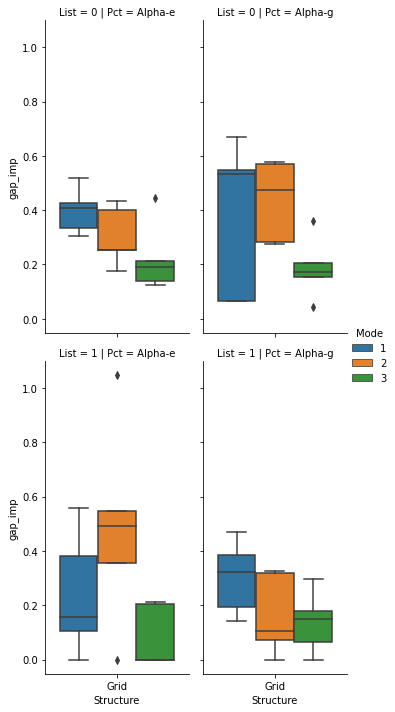
\includegraphics[width=0.35\linewidth]{improved_gap_ND.png}
        \caption{Matheuristic improved gap for the NMDRPG}
        \label{fig:4}
        \end{figure}
	\end{frame}
	

	\section{Coordinated Models: The AMMDRPG}
	\begin{frame}{Contents}
	    \begin{itemize}
		    \item Problem Description
		    \item Formulations
		    \item Example
		    \item Strengthening the formulation
		    \item Matheuristic
		    \item Computational Experiments
		    \item Case Study
		\end{itemize}
	\end{frame}
	
	\begin{frame}{Problem Description}
	\begin{itemize}
	    \item There is one mothership and a fleet of drones in coordination to visit a set of target graphs, whose locations are given. \textcolor{red}{The drone has a limited endurance $N^d$ in this case}.
	    \item For each graph $g\in\mathcal G$ the assigned drone performs the following task:
	    \begin{enumerate}
	        \item It is launched from the current mothership location (to be determined).
	        \item It flies to the graph $g$ that has to be visited.
	        \item It traverses the required edges of graph $g$.
	        \item It returns to the current position of the mothership (to be determined).
	    \end{enumerate}
	    We assume wlog that the mothership and the drone do not need to arrive at each rendezvous location at the same time: the fastest arriving vehicle may wait for the other at the rendezvous point.
	\end{itemize}
	\end{frame}
	
	\begin{frame}{Problem Description}
	It is required to determine:
	    \begin{itemize}
	        \item The tour of the mothership starting at $orig$, deciding the different launching and rendezvous points, and returning to $dest$.
	        \item The optimal assignment of drones for visiting graphs in a given stage $t$.
	        \item The order of visits of the target graphs followed by the drone, determining the corresponding launching and rendezvous points of the drone on each visited graph.
	        \item The tour followed by the drone on each target graph $g \in \mathcal{G}$.
	    \end{itemize}
	\end{frame}
	
	\begin{frame}{Parameters of the AMMDRPG}
	\footnotesize
	The known parameters of the problem are:
	\begin{itemize}
	    \item $orig$: coordinates of the point defining the origin of the mothership path (or tour).
        \item $dest$: coordinates of the point defining the destination of the mothership path (or tour).
        \item $\mathcal{G}$: set of the target graphs.\\
        \item $g = (V_g, E_g)$: set of nodes and edges of each target graph $g \in \mathcal{G}$.
        \item $\mathcal{L}(e_g)$: length of edge $e$ of graph $g \in \mathcal{G}$.
        \item $B^{e_g}, C^{e_g}$: coordinates of the endpoints of edge $e$ of graph $g \in \mathcal{G}$.
        \item $\alpha^{e_g}$: percentage of edge $e$ of graph $g \in \mathcal{G}$ that must be visited.
        \item $\alpha^g$: percentage of graph $g \in \mathcal{G}$ that must be visited.
        \item $v_D$: drone speed.
        \item $v_M$: mothership speed.
        \item $N^d$: drone endurance.
        \item $M$: big-M constant.
    \end{itemize}
	\end{frame}
	
	\begin{frame}{Binary and Integer Decision Variables for the AMMDRPG}
	\begin{itemize}
	    \item $\mu^{e_g} \in \{0,1\} \:\: \forall e_g \in E_g$ ($g \in \mathcal{G}$): equal to 1 if edge $e$ of graph $g$ (or a portion of it) is visited by the drone, and  0 otherwise.
        \item $entry^{e_g} \in \{0,1\} \:\: \forall e_g \in E_g$ ($g \in \mathcal{G}$): auxiliary binary variable used for linearizing expressions.
        \item $u^{e_{g}td} \in \{0,1\} \:\: \forall e_g \in E_g$ ($g \in \mathcal{G}$) $\: \forall t \in \mathcal T$: equal to 1 \textcolor{red}{if the drone $d$} enters in graph $g$ by the edge $e_g$ at stage $t$, 0 otherwise.
        \item $z^{e_{g}e^{'}_{g}} \in \{0,1\} \:\: \forall e_g, e_g' \in E_g$ ($g \in \mathcal{G}$): equal to 1 if the drone goes from $e_g$ to $e^{'}_{g}$, 0 otherwise.
        \item $v^{e_{g}td} \in \{0,1\} \:\: \forall e_g \in E_g$ ($g \in \mathcal{G}$) $\: \forall t \in \mathcal T$: equal to 1 \textcolor{red}{if the drone $d$} exits from graph $g$ by $e_g$ at stage $t$, 0 otherwise.
        \item $s^{e_g},\; \forall e_g \in E_g$ ($g \in \mathcal{G}$): integer non negative variable representing the order of visit of edge $e$.
    \end{itemize}
	\end{frame}
	
	\begin{frame}{Continuous Decision Variables for the AMMDRPG}
	\textbf{Location variables}
	\begin{itemize}
	    \item $\rho^{e_g} \in [0,1]$ and $\lambda^{e_g} \in [0,1] \:\: \forall e_g \in E_g$ ($g \in \mathcal{G}$): defining the entry and exit points on $e_g$.
        \item $\nu_\text{min}^{e_g}$ and $\nu_\text{max}^{e_g} \in [0,1] \forall e_g \in E_g$ ($g \in \mathcal{G}$): auxiliary variables used for linearizing expressions.
        \item $x_L^t \:\: \forall t \in \mathcal T$: coordinates representing the point where the mothership launches the drone at stage $t$.
        \item $x_R^t \:\: \forall t \in \mathcal T$: coordinates representing the point where the mothership retrieves the drone at stage $t$.
        \item $R^{e_g} \:\: \forall e_g \in E_g$ ($g \in \mathcal{G}$): coordinates representing the entry point on edge $e$ of graph $g$.
        \item $L^{e_g} \:\: \forall e_g \in E_g$ ($g \in \mathcal{G})$: coordinates representing the exit point on edge $e$ of graph $g$.
    \end{itemize}
    \end{frame}
    
    \begin{frame}{Continuous Decision Variables for the AMMDRPG}
    \textbf{Distance variables}
    \begin{itemize}
        \footnotesize
        \item $d_L^{e_gtd} \geq 0, \:\: \forall e_g \in E_g$ ($g \in \mathcal{G}$) $\forall t \in \mathcal T$: representing the distance travelled by the \textcolor{red}{drone $d$} from the launching point $x_L^t$ on the mothership at stage $t$ to the first visiting point $R^{e_g}$ on $e_g$.
        \item $d^{e_ge^\prime_g} \geq 0, \:\: \forall e_g, e^\prime_g \in E_g $ ($g \in \mathcal{G}$): representing the distance travelled by the drone from the launching
        point $L^{e_g}$ on $e_g$ to the rendezvous point $R^{e^\prime_g}$ on $e^\prime_g$.
        \item $d^{e_g} \geq 0, \:\: \forall e_g \in E_g$ ($g \in \mathcal{G}$): representing the distance travelled by the drone from the rendezvous point $R^{e_g}$ to the launching point $L^{e_g}$ on $e_g$. 
        \item $d_R^{e_gtd} \geq 0 \:\: \forall e_g \in E_g$ ($g \in \mathcal{G}$) $\forall t \in \mathcal T$: representing the distance travelled by the \textcolor{red}{drone $d$} from the last
        visiting point $L^{e_g}$ on $e_g$ to the rendezvous point $x_R^t$ on the mothership at stage $t$.
        \item $d_{LR}^t \geq 0 \:\: \forall t \in \mathcal T$: representing the distance travelled by the mothership from the launching point $x_L^t$ to the rendezvous point $x_R^t$ at stage $t$.
        \item $d_{RL}^t \geq 0 \:\: \forall t \in \mathcal T$: representing the distance travelled by the mothership from the rendezvous point $x_R^t$ at stage $t$ to the launching point $x_L^{(t+1)}$ at the stage $t+1$.
    \end{itemize}
	\end{frame}

    \begin{frame}{Visit of the graphs}
	    We have considered two modes of visit to the target graphs $g\in \mathcal{G}$ that must be represented by their corresponding constraints:
        \begin{itemize}
            \item Visiting a percentage $\alpha^{e_g}$ of each edge $e_g$ which can be modeled by:
            \begin{equation}\label{eq:alphaE}\tag{$\alpha$-E}
            |\lambda^{e_g} - \rho^{e_g}|\mu^{e_g}\geq \alpha^{e_g}, \quad \forall e_g\in E_g.
            \end{equation}
            \item Visiting a percentage $\alpha^g$ of the total length $\mathcal L(g)$ of the graph $g$ modeled by:
            \begin{equation}\label{eq:alphaG}\tag{$\alpha$-G}
            \sum_{e_g\in E_g} \mu^{e_g}|\lambda^{e_g} - \rho^{e_g}|\mathcal L(e_g) \geq \alpha^g\mathcal L(g).
            \end{equation}
            %where $\mathcal L(g)$ denotes the total length of the graph.
        \end{itemize}
	\end{frame}
	
	\begin{frame}{Visit of the graphs}
	    In both cases the corresponding constraints are nonlinear. For each edge $e_g$, we linearize the absolute value constraint \eqref{eq:alphaE} by introducing a binary variable:
        \begin{equation}\label{eq:alpha-E}\tag{$\alpha$-E}
         \mu^{e_g}|\rho^{e_g}-\lambda^{e_g}|\geq \alpha^{e_g} \Longleftrightarrow
         \left\{
         \begin{array}{ccl}
          \rho^{e_g} - \lambda^{e_g}                       & =    & \nu_\text{max}^{e_g} - \nu_\text{min}^{e_g}                                     \\
          \nu_\text{max}^{e_g}                         & \leq & 1-{\text{entry}^{e_g}}                                    \\
          \nu_\text{min}^{e_g}                      & \leq & {  \text{entry}^{e_g}},                                        \\
          \mu^{e_g}(\nu_\text{max}^{e_g} + \nu_\text{min}^{e_g} ) & \geq & \alpha^{e_g}.
          \\
         \end{array}
         \right.
        \end{equation}
        
        \noindent
        The linearization of \eqref{eq:alphaG} is similar to \eqref{eq:alphaE} and only requires changing the last inequality in \eqref{eq:alpha-E} for
        
        \begin{equation}\label{eq:alpha-G}\tag{$\alpha$-G}
        \sum_{e_g\in E_g} \mu^{e_g}(\nu_\text{max}^{e_g} + \nu_\text{min}^{e_g})\mathcal L(e_g)\geq \alpha_g\mathcal L(g).
        \end{equation}
	\end{frame}
	
	\begin{frame}{Modeling the Drone Route}
	\begin{small}
    {\color{red}
    \begin{align}
        \sum_{g\in \mathcal G}\sum_{e_g\in E_g} \sum_{d\in\mathcal D} u^{e_gtd} & \leq 1, &\forall t\in \mathcal T, \label{st:DEntd}\\%\tag{DEn}\\
        \sum_{g\in\mathcal G}\sum_{e_g\in E_g} \sum_{d\in\mathcal D} v^{e_gtd} & \leq 1, &\forall t\in \mathcal T, \label{st:DExtd}\\%\tag{DEx}\\
        \sum_{e_g\in E_g} \sum_{t\in \mathcal T} \sum_{d\in\mathcal D} u^{e_gtd} & = 1, &\forall g\in\mathcal G, \label{st:DEngd}\\%\tag{D
        \sum_{e_g\in E_g} \sum_{t\in \mathcal T} \sum_{d\in\mathcal D} v^{e_gtd} & = 1, &\forall g\in\mathcal G, \label{st:DExgd}\\%\tag{D
        \sum_{e_g\in E_g} u^{e_gtd} & = \sum_{e_g\in E_g} v^{e_gtd}, &\forall g\in\mathcal G, \forall t\in \mathcal T, \forall d\in\mathcal D, \label{st:Duvd}\\%\tag{D
         \sum_{t\in \mathcal T} \sum_{d \in \mathcal D} u^{e_gtd} + \sum_{e^\prime_g\in E_g} z_g^{e^\prime_ge_g} & = \mu^{e_g}, &\forall e_g\in E_g:g\in\mathcal G, \label{st:DInud}\\
         \sum_{t\in \mathcal T} \sum_{d \in \mathcal D} v^{e_gtd} + \sum_{e^\prime_g\in E_g} z_g^{e_ge^\prime_g} & = \mu^{e_g}, &\forall e_g\in E_g:g\in\mathcal G. \label{st:DInvd}
    \end{align}}
    \end{small}
	\end{frame}
	
	\begin{frame}{Subtour elimination inside the graph}
	    \begin{small}
		To prevent the existence of subtours within each graph $g\in \mathcal G$ that the drone must visit: 
		\begin{itemize}
		\item One can add the Miller-Tucker-Zemlin constraints, given by:
    		\begin{align}
    		    s^{e_g} - s^{e^\prime_g} + |E_g|z^{e_ge^\prime_g} & \leq |E_g| - 1  , &\quad\forall e_g \neq e_g'\in E_g \tag{MTZ$_1$}, \label{MTZ1}\\
                0 & \leq s^{e_g} \leq |E_g| - 1, &\quad\forall e_g\in E_g\tag{MTZ$_2$},\label{MTZ2}
                \end{align}
        \item It is also possible to include the subtour elimination constraints:
        \begin{equation}\tag{SEC}\label{SEC}
        \sum_{e_g, e^\prime_g \in S} z_g^{e_ge^\prime_g} \leq |S| - 1, \quad \forall S\subset E_g:g\in \mathcal G.
    \end{equation}
    \end{itemize}
    \end{small}
	    
	\end{frame}
	
	\begin{frame}{Distance constraints}
	    To account for the different distances among the decision variables of the model we need to set the continuous variables $d_L^{e_gt}$, $d^{e_g}$, $d^{e_ge^\prime_g}$, $d_R^{e_gt}$, $d_{RL}^t$ and $d_{LR}^t$. This can be done by means of the following constraints:
        
        \begin{align*}
        \|x_L^t- R^{e_g}\| & \leq  d_L^{e_gtd},  &\quad \forall e_g:g\in \mathcal{G}, \forall t\in \mathcal T, \forall d\in\mathcal D, \tag{DIST$_{1}$-t} \label{eq:d1d}\\
        \|R^{e_g}- L^{e_g}\| & \leq  d^{e_g},  &\quad \forall e_g:g\in \mathcal{G}, \tag{DIST$_{2}$-t} \label{eq:d2}\\
        \|R^{e_g}- L^{e^\prime_g}\| & \leq  d^{e_ge^\prime_g}, &\quad \forall e_g\neq e_g'\in E_g:g\in \mathcal{G}, \tag{DIST$_{3}$-t} \label{eq:d3}\\
        \|L^{e_g}- x_R^t\| & \leq  d_R^{e_gtd}, &\quad \forall e_g:g\in \mathcal{G},\forall t\in T, \forall d\in\mathcal D, \tag{DIST$_{4}$-t} \label{eq:d4}\\
        \|x_R^t- x_L^{t+1}\| & \leq  d_{RL}^t, & \quad \forall t\in \mathcal T, \tag{DIST$_{5}$-t} \label{eq:d5}\\
        \|x_L^t- x_R^t\| & \leq  d_{LR}^t, & \quad \forall t\in \mathcal T. \tag{DIST$_{6}$-t} \label{eq:d6d}\\
        \end{align*}
	\end{frame}
	
	\begin{frame}{Coordination constraint}
        The coordination between the drones and the mothership must ensure that the time spent by the drone $d$ to visit the graph $g$ at the stage $t$ is less than or equal to the time that the mothership needs to move from the launching point to the retrieving point during the stage $t$. To this end, we need to define the following coordination constraint for each graph $g\in \mathcal G$, stage $t\in \mathcal T$ and drone $d\in\mathcal D$:
        
        \begin{tiny}
        {\color{red}
        \begin{equation}\tag{DCW}\label{DCW}
        \frac{1}{v_D}\left(\sum_{e_g\in E_g} u^{e_gtd}d_L^{e_gtd} + \sum_{e_g, e^\prime_g\in E_g}z^{e_ge^\prime_g}d^{e_ge^\prime_g} + \sum_{e_g\in E_g} \mu^{e_g}d^{e_g} + \sum_{e_g\in E_g} v^{e_gtd}d_R^{e_gtd}\right) \leq \frac{d_{LR}^t}{v_M} + M(1 - \sum_{e_g\in E_g} u^{e_gtd}).
        \end{equation}}
        \end{tiny}
	\end{frame}
	
	\begin{frame}{Endurance constraint}
    	Note that, since the objective function of this problem minimizes the right-hand-side of \eqref{DCW}, this constraint will become an equality and we can model the time capacity constraint for a particular stage $t\in \mathcal T$ by limiting the distance traveled by the mothership for this task $t$:
    
    {\color{red}
    \begin{equation}\tag{Capacity}\label{CAP}
        d_{LR}^t \leq N^d.
    \end{equation}}
	    
	\end{frame}
	\begin{frame}{Setting the origin and the destination}
	    Eventually, we have to impose that the tour of the mothership, together with the drone, starts from the origin $orig$ and ends at the destination $dest$. To this end, we define the following constraints:

        \begin{align*}
        x_L^0 & =  orig,  \tag{ORIG$_1$} \label{eq:O1} \\
        x_R^0 & =  orig,  \tag{ORIG$_2$} \label{eq:O2} \\
        x_L^{|\mathcal{G}|+1} & =  dest,  \tag{DEST$_1$} \label{eq:D1} \\
        x_R^{|\mathcal{G}|+1} & =  dest.  \tag{DEST$_2$} \label{eq:D2} 
        \end{align*}

	\end{frame}
	
	\begin{frame}{Formulation for the AMMDRPG}
	
	\begin{align*}
	    \text{min}\quad & \sum_{t\in \mathcal T} (d_{RL}^t + d_{LR}^t) \\
	    \text{s.t.}\quad & \eqref{st:DEntd}-\eqref{st:DInvd}, \\
	    & \eqref{MTZ1} - \eqref{MTZ2} \text{ or } \eqref{SEC}, \\
	    & \eqref{eq:alpha-E} \text{ or } \eqref{eq:alpha-G}, \\
	    & \eqref{DCW}, \textcolor{red}{\eqref{CAP}}, \\
	    & \eqref{eq:d1d}-\eqref{eq:d6d}, \\
	    & \eqref{eq:O1}-\eqref{eq:D2}.
	\end{align*}
	\end{frame}
	
	\begin{frame}{Example}
        \begin{figure}
        \centering
        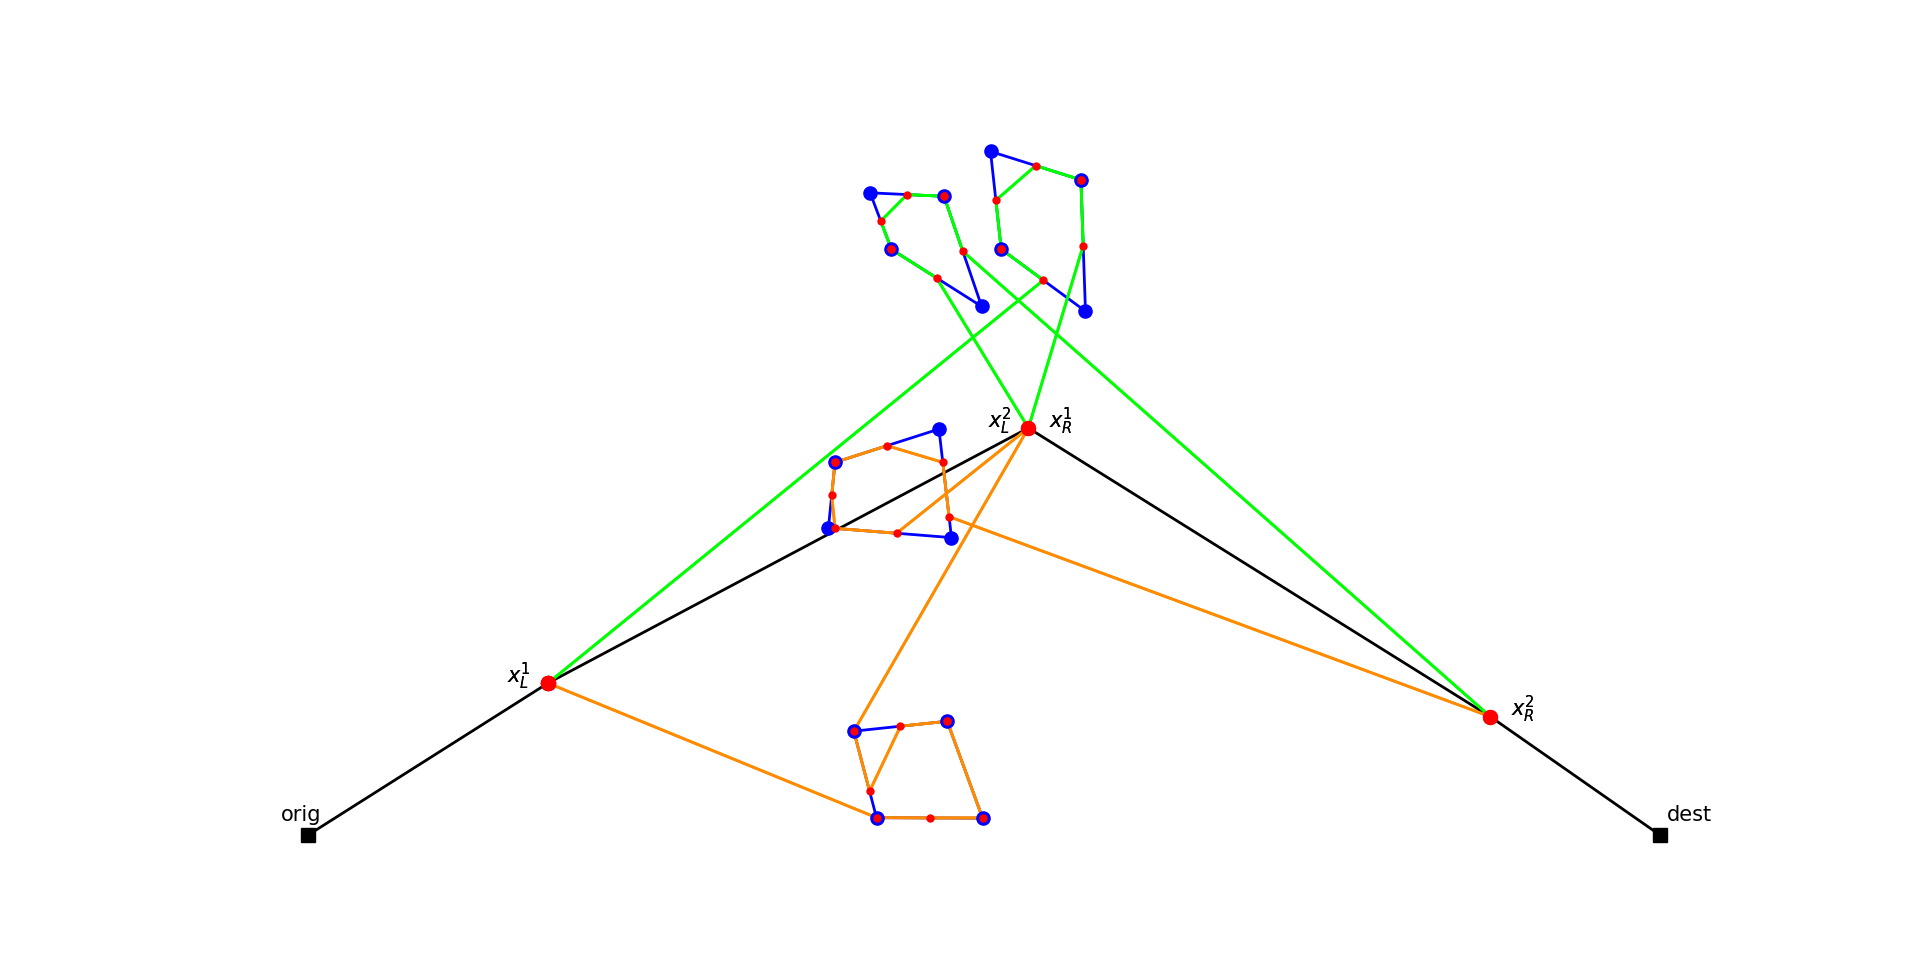
\includegraphics[width=0.95\linewidth]{figure_latex.png}
        \caption{Example illustrating the meaning of the launching  (L) and retrieving (R) points.}
        \label{fig:illustrative}
        \end{figure}
	\end{frame}
	
	\begin{frame}{The AMMDRPG without synchronisation}
	    We consider a variant of the model presented before, in which we assume that the mothership can retrieve one drone in a stage different from the one in which it has been launched. That is, the mothership can move to another point to launch a new drone without having  retrieved the one that was launched before.
        \bigskip
        
        To deal with this extension, we do not need to define new variables since it is possible to use the same variables that were used in the previous model. \\
        
        First of all, constraint \eqref{st:Duvd} must be changed to:
        {\color{red}
        \begin{equation}\label{constraint:Duv-S}
            \sum_{e_g\in E_g} u^{e_gtd} -  \sum_{e_g\in E_g} \sum_{t'\geq t} v^{e_gt'd}=0, \quad\forall  g\in\mathcal G,\forall t\in\mathcal T, \forall d\in\mathcal D.
        \end{equation}}

	\end{frame}
	
	\begin{frame}{The AMMDRPG without synchronisation}
		\small
       Moreover, the coordination constraint \eqref{DCW} must be modified to consider the general case in which the stages of launching and retrieving can be different. For each $t_1<t_2$ and $\forall g\in\mathcal G,\forall d\in\mathcal D$:
       \begin{itemize}
            
           \item Time spent by the drone $d$ to visit the graph $g$:
           \begin{scriptsize}
              $$T_D = \frac{1}{v_D}\left(\sum_{e_g\in E_g} u^{e_gt_1d}d_L^{e_gt_1d} + \sum_{e_g, e^\prime_g\in E_g}z^{e_ge^\prime_g}d^{e_ge^\prime_g} & + \sum_{e_g\in E_g} \mu^{e_g}d^{e_g} + \sum_{e_g\in E_g} v^{e_gt_2d}d_R^{e_gt_2d}\right).$$
           \end{scriptsize}

           \item Time spent by the mothership:
           {\color{red}
           $$T_M = \frac{\sum_{t=t_1}^{t_2}d_{LR}^t}{v_M} + \frac{\sum_{t=t_1}^{t_2-1}d_{RL}^t}{v_M} + M(2 - \sum_{e_g\in E_g} u^{e_gt_1d} - \sum_{e_g\in E_g} v^{e_gt_2d}).$$}
       \end{itemize}
       
       The time spent by the drone must be lower than the one spent by the mothership:
       \begin{equation}\tag{DCW-NS}\label{constraint:DCW-NS}
            T_D \leq T_M.
        \end{equation}
	\end{frame}
	
	\begin{frame}{\large Link between AMMDRPG with and without synchronisation}
	
	\begin{theorem}
        Let $x_L^1$, $x_L^2$ (resp. $x_R^1$, $x_R^2$) be the launching (resp. rendezvous) points associated to the visit of the target points $P_1$ and $P_2$. If there exist two points $x_L$ and $x_R$ verifying 
        $$
         \left\{
         \begin{array}{ccl}
          \dfrac{\|x_L-x_R\|}{v_C} & \leq    & \dfrac{\|x_L - P_1\| + \|P_1 - x_R\|}{v_D}, \\
          \dfrac{\|x_L-x_R\|}{v_C} & \leq    & \dfrac{\|x_L - P_2\| + \|P_2 - x_R\|}{v_D}, \\
          \dfrac{\|x_L-x_R\|}{v_C} & \leq   & N^d, \\
          \|x_L-x_R\| & \leq & \|x_L^1 - x_L^2\| + \|x_L^2- x_R^1\| + \|x_R^1-x_R^2\|,
         \end{array}
         \right.
        $$
        
        \noindent then the contribution of this partial route to the optimal objective value will be the same in both models.
        \end{theorem}
	    
	\end{frame}
	
	\begin{frame}{Valid inequalities for the AMMDRPG}
	\begin{itemize}
	    \item Let $\beta^t$ be a binary variable that assumes the value one if all the target graphs are visited when the operation $t$ begins, and  zero, otherwise.
	    \begin{equation}\tag{Monotonicity}\label{eq:Monotonicity}
            \beta^t \leq \beta^{t+1}, \mbox{ for all } t=1,\ldots, |\mathcal{G}|-1.
        \end{equation}
	    \item Let $k^t$ denote the number of graphs that are visited in the stage $t$. 
	    $$k^t=\sum_{e_g\in g:g\in\mathcal G}\sum_{d\in\mathcal D} u^{e_gtd}.$$
	\end{itemize}
	\end{frame}
	
	\begin{frame}{Valid inequalities for the AMMDRPG}
	    \begin{block}{Valid Inequalities I}
	    If $\beta^t$ is one, the entire set of graphs in $\mathcal G$ must have been visited before the stage $t$:
            \begin{equation}\tag{VI-1}\label{eq:VI-1}
            \sum_{t'=1}^{t-1} k^{t'} \geq |\mathcal G|\beta^t.
            \end{equation}
        \end{block}
        
        \begin{block}{Valid Inequalities II}
        It is not permitted to have a stage $t$ without any operation if some graphs are still to be visited:
            \begin{equation}\tag{VI-2}\label{eq:VI-2}
            k^t \geq 1 - \beta^t.
            \end{equation}
        \end{block}
    \end{frame}
    
    \begin{frame}{Valid inequalities for the AMMDRPG}
        \begin{block}{Valid Inequalities III and IV}
        We are assuming that drones are indistinguishable, we can assume that given an arbitrary order on them, we always assign drones to operations in that given order. For all $t=1,\ldots,|\mathcal G|:$
        \begin{equation}\tag{VI-3}\label{eq:VI-3}
        \sum_{e_g\in \mathcal G} u^{e_gtd} \leq \sum_{e_g:g\in\mathcal G}u^{e_gtd-1}, \; \forall d=2,\ldots |\mathcal D|,      
        \end{equation}
        \begin{equation}\tag{VI-4}\label{eq:VI-4}
        \sum_{e_g\in \mathcal G} v^{e_gtd} \leq \sum_{e_g:g\in\mathcal G}v^{e_gtd-1}, \; \forall d=2,\ldots |\mathcal D|.      
        \end{equation}
        \end{block}
    \end{frame}
	
	\begin{frame}{Adjusting the Big-M constants}
    The model that we have proposed includes big-M constants. We have defined different big-M constants along this work. In order to strengthen the formulations we provide tight upper and lower bounds for those constants:
    
    \begin{block}{Big-M constants bounding $d_L^{e_gtd}$ and $d_R^{e_gtd}$}
    \small
        We model the product $d_L^{e_gtd} u_L^{e_gtd}$ by defining the auxiliar non-negative continuous variables $p_L^{e_gtd}$ (resp. $p_R^{e_gtd}$) and including the following constraints:
        \begin{align*}
        p_L^{e_gtd} & \geq m_L^{e_g} u^{e_gtd}, \\
        p_L^{e_gtd} & \leq d_L^{e_g} - M_L^{e_gtd}(1-u^{e_gt}).
        \end{align*}
        The best upper bound $M_L^{e_gtd}$ or $M_R^{e_gtd}$ that we can consider is the maximum distance between every pair of vertices of the graphs $g\in \mathcal{G}$:
        $$
        M_R^{e_gtd} = \max_{\{v\in V_g, v'\in V_{g'} : g, g'\in\mathcal G\}} \|v - v'\| = M_L^{e_gtd}.
        $$
    \end{block}
	\end{frame}
	
	\begin{frame}{Adjusting the Big-M constants}
    The model that we have proposed includes big-M constants. We have defined different big-M constants along this work. In order to strengthen the formulations we provide tight upper and lower bounds for those constants:
    
    \begin{block}{Big-M constants bounding $d^{e_ge'_g}$}
        \footnotesize
        We model the product $d^{e_ge_g'} z^{e_g e_g'}$ by defining the auxiliar non-negative continuous variables $p^{e_ge_g'}$ and including the following constraints:
        \begin{align*}
        p^{e_ge'_g} & \geq m^{e_ge_g'} d_{RL}^{gg'}, \\
        p^{e_ge_g'} & \leq d^{e_ge_g'} - M^{e_ge_g'}(1-z^{e_ge_g'}).
        \end{align*}
        Since we are taking into account the distance between two edges $e=(B^{e_g},C^{e_g}), \, e'=(B^{e^\prime_g},C^{e^\prime_g})\in E_g$, the maximum and minimum distances between their vertices give us the upper and lower bounds:
        \begin{align*}
        M^{e_g e^\prime_g} = & \max\{\|B^{e_g} - C^{e^\prime_g}\|, \|B^{e_g} - B^{e^\prime_g}\|, \|C^{e_g} - B^{e^\prime_g}\|, \|C^{e_g} - C^{j_g}\|\}, \\
        m^{e_g e^\prime_g} = & \min\{\|B^{e_g} - C^{e^\prime_g}\|, \|B^{e_g} - B^{e^\prime_g}\|, \|C^{e_g} - B^{e^\prime_g}\|, \|C^{e_g} - C^{e^\prime_g}\|\}.
        \end{align*}
    \end{block}
	\end{frame}
	
	\begin{frame}{Adjusting the Big-M constants}
    The model that we have proposed includes big-M constants. We have defined different big-M constants along this work. In order to strengthen the formulations we provide tight upper and lower bounds for those constants:
    
    \begin{block}{Big-M constants bounding the total distance made by a drone in a stage}
        \footnotesize
        To link the drone operation with the trip followed by the mothership, we have defined the constraint $\eqref{DCW}$ that includes another big-M constant.
        
        \bigskip
        
        To obtain an upper bound on $M$ we add to the length of the graph $\mathcal L(g)$ the big-Ms computed for $u^{e_gtd}$ and $v^{e_gtd}$, namely $M_{L}^{e_gtd}$ and $M_R^{e_gtd}$, respectively, and the maximum distance that can be traveled by the drone to move from one edge to another one. This results in a valid value for this $M$ constant:
        
        $$M = \mathcal{L}(g) + M_L^{e_gtd} + M_R^{e_gtd} + \sum_{e_g, e_g'\in E_g}M^{e_ge_g'}.$$
    \end{block}
	\end{frame}
	
	\begin{frame}{Matheuristic for the AMMDRPG}
	   \textbf{Pseudo-code of this algorithm:}
        \begin{itemize} 
        \item[STEP 1] (First entry and last exit points for each target graph)\\
        Compute the route on each target graph $g \in \mathcal{G}$.
        Let $L^{e_{g}}$ and $R^{e^{'}_{g}}$ be the pair of entry and exit points on $g$ closest to the origin and let  $\mathcal L(e_{g}, e^{'}_{g})$ be the associated length computed as the sum of the distances travelled by the drone to visit the graph $g$, excluding the distance between $L^{e_{g}}$ and $R^{e^{'}_{g}}$.
        \end{itemize}
    \end{frame}
    \begin{frame}{Matheuristic for the AMMDRPG}
    	\textbf{Pseudo-code of this algorithm:}
        \begin{itemize}
        \small
        \item[STEP 2] (Clustering procedure)\\
        Initialization: set $it=1$, define one cluster for each target graph and set $nit=1$. \\
        Select randomly two clusters $K_i$ and $K_j$ (where $i<j$).\\
        Check if the number of graphs belonging to the union of $K_i$ and $K_j$ is less than the number of available drones $n_D$.\\
        If this condition is satisfied:\\
        search for point $P$ satisfying the following capacity constraint:
        $$
        \frac{d(P, R^{e_g}) + \mathcal L(e_{g}, e^{'}_{g}) + d(L^{e^{'}_{g}}, P)}{v_D} \leq N^d, \quad \forall R^{e_g}, L^{e^{'}_{g}} \in K_i, \:\: K_j.
        $$
        If such a point exists, merge the two clusters and label the new one as $K_i$.\\
        Set $nit=nit+1$.\\
        Repeat the same procedure on the new cluster structure while $nit < maxit$.
        \end{itemize}
    \end{frame}
    
    \begin{frame}{Matheuristic for the AMMDRPG}
    \textbf{Pseudo-code of this algorithm:}
    \begin{itemize}
        \small
        \item[STEP 3] (Computation of Reference Points) 
        %\JP{This step is not well-defined: The term centroid defines exactly the points we should use another term that allows to minimize something!!!} \\
        % Compute the centroids of the clusters generated at STEP 2, by minimizing the distance between them and the origin always imposing that the capacity constraint is satisfied.
        Compute a reference point for each cluster generated at STEP 2. This computation seeks for the minimization of the distance between each pair of reference points and the distance between them and the origin, always imposing that the \eqref{CAP} constraint is satisfied.
        \item [STEP 4] (Setting the order of visits to the  graphs: route via the reference points and the origin/destination points) \\
        Compute the TSP of the mothership among the reference points of the clusters and let $\mathcal L(TSP)$ be the associated length.\\
        Set $it=it+1$.\\
        if(it< maxseed) go to STEP 2\\
        else go to STEP 5
        \item [STEP 5] (Solution of the AMMDRPG model fixing an initial partial solution)\\
        Set the values of the binary variables $u^{e_{g}td}$ and $v^{e_{g}td}$ and solve the model \AMD\, to obtain a feasible solution.
    \end{itemize}
	\end{frame}
	
	\begin{frame}{Experiment 1}
    We generate five instances for each setting:
    \begin{itemize}
        \item Number of target graphs $|\mathcal G|\in\{5, 10\}$.
        \item The same percentage of graphs ($20\%$) has respectively 4, 6, 8, 10 and 12 nodes.
        \item Number of drones $n_D\in\{1, 2, 3\}.$
        \item Drone endurance $N^d\in\{20, 30, 40, 50, 60\}$.
        \item $v_D= 2v_M$.
        \item $\alpha^g$ and $\alpha^{e_g}$ randomly generated in $[0, 1]$.
    \end{itemize}
    
    The experiment consists on:
    \begin{itemize}
        \item Running the formulation for (AMMDRPG) with and without initial solution provided by the matheuristic.
        \item Using Gurobi 10.1.
        \item Time Limit: 2 hours.
    \end{itemize}
    \end{frame}
	
	\begin{frame}{Experiment 1: Results}
        \begin{table}
        \caption{Comparison between exact solution with and without initialization by the matheuristic solution}
        \centering
        \tiny
        \resizebox{\textwidth}{!}{
        \begin{tabular}{|c|c|c|c c c c c c c c c|}
        \hline
        \multirow{3}{*}{\textbf{|$\mathcal{G}$|}} & \multirow{3}{*}{\textbf{N^d}}  & \multirow{3}{*}{\textbf{v.t.}} & \multicolumn{9}{|c|}{\textbf{$\#$ drones}} \\
        \cline{4-12}
        & & & \multicolumn{3}{c|}{1} & \multicolumn{3}{c|}{2} & \multicolumn{3}{c|}{3}\\
        \cline{4-12}
        & & &  $\%$Gap (i) & TimeH & $\%$Gap (wi) & $\%$Gap (i) & TimeH & $\%$Gap (wi)& $\%$Gap (i) & TimeH & $\%$Gap (wi)\\
        \hline
        \multirow{5}{*}{\midrule 5} & \multirow{2}{*}{20} & e & 82,63 & 61,56 & 81,70 & 91,57 &	63,80 &	90,61 &	93,06 &	60,87 &	90,93\\
        &  & g & 79,09 & 44,97 & 79,63 & 89,03 & 37,32 & 91,85 & 94,00 & 39,05 & 95,80\\
        \cline{2-12}
        & \multirow{2}{*}{30} & e & 82,70 &	65,21 &	80,17 &	85,14 &	64,41 &	82,21 &	91,90 &	63,34 &	90,12\\
        & & g & 75,80 &	55,77 &	71,19 &	84,36 &	44,36 &	88,27 &	91,02 &	44,59 &	91,39\\
        \cline{2-12}
        & \multirow{2}{*}{40} & e & 80,94 &	68,81 &	77,98 &	83,44 &	64,80 &	82,16 &	91,24 &	63,19 &	86,25\\
        & & g & 74,47 &	43,92 &	73,46 &	81,21 &	38,27 &	84,35 &	85,34 &	37,51 &	89,63\\
        \cline{2-12}
        & \multirow{2}{*}{50} & e & 76,87 &	66,67 &	74,41 &	81,12 &	63,86 &	79,57 &	85,11 &	63,51 &	86,16\\
        & & g & 70,58 &	43,42 &	66,90 &	80,96 &	43,98 &	88,84 &	80,49 &	44,35 &	82,81\\
        \cline{2-12}
        & \multirow{2}{*}{60} & e & 76,39 &	67,78 &	71,61 &	81,63 &	66,08 &	79,84 &	83,82 &	64,40 &	82,06\\
        & & g & 78,17 &	44,69 &	72,79 &	79,35 &	40,63 &	86,55 &	81,74 &	50,01 &	84,66\\
        \hline
        \multirow{5}{*}{10} & \multirow{2}{*}{20} & e & 82,56 &	137,93 &	84,91 &	92,30 &	128,53 & - & 94,73 & 124,44 & -\\
        &  & g & 81,00 & 119,20 & \textcolor{red}{84,08 (2)} & 89,88 & 83,50 & \textcolor{red}{96,64 (2)} & 96,44 & 70,00 & \textcolor{red}{97,43 (3)}\\
        \cline{2-12}
        & \multirow{2}{*}{30} & e & 80,60 &	159,00 & 80,93 & 87,11 & 132,15 & \textcolor{red}{87,58 (3)} &	94,56 &	127,35 & \textcolor{red}{92,85 (2)}\\
        & & g & 79,93 &	132,67 & \textcolor{red}{82,70 (1)} & 86,32 & 80,29 & \textcolor{red}{86,13 (3)} & 91,12 &	76,72 &	\textcolor{red}{89,74 (1)}\\
        \cline{2-12}
        & \multirow{2}{*}{40} & e & 79,05 &	191,37 & 78,07 & 85,11 & 131,26 &	84,33 &	91,88 &	132,10 & \textcolor{red}{88,61 (1)}\\
        & & g & 80,23 &	115,00 & 79,64 & 87,31 & 68,39 & \textcolor{red}{84,57 (3)} & 96,09 &	69,40 &	\textcolor{red}{91,86 (1)}\\
        \cline{2-12}
        & \multirow{2}{*}{50} & e & 81,49 &	188,32 & 77,81 & 87,72 & 134,01 &	\textcolor{red}{85,51 (1)} &	92,68 &	132,82 & \textcolor{red}{90,79 (3)}\\
        & & g & 79,92 &	87,23 &	80,38 &	82,80 &	66,14 &	\textcolor{red}{84,00 (3)} &	92,48 &	64,94 &	\textcolor{red}{91,96 (2)}\\
        \cline{2-12}
        & \multirow{2}{*}{60} & e & 83,79 &	155,27 & 81,57 & 85,91 & 131,94 &	\textcolor{red}{82,96 (2)} &	92,24 &	130,11 & \textcolor{red}{86,58 (3)}\\
        & & g & 77,57 &	97,89 &	78,46 &	86,94 &	76,53 &	\textcolor{red}{88,29 (2)} &	94,31 &	69,53 &	\textcolor{red}{92,23 (3)}\\
        \hline
        \end{tabular}}
        \label{table:tab2}
        \end{table}
	\end{frame}
	
	\begin{frame}{Experiment 1: Results}
	    \begin{figure}[h!]
        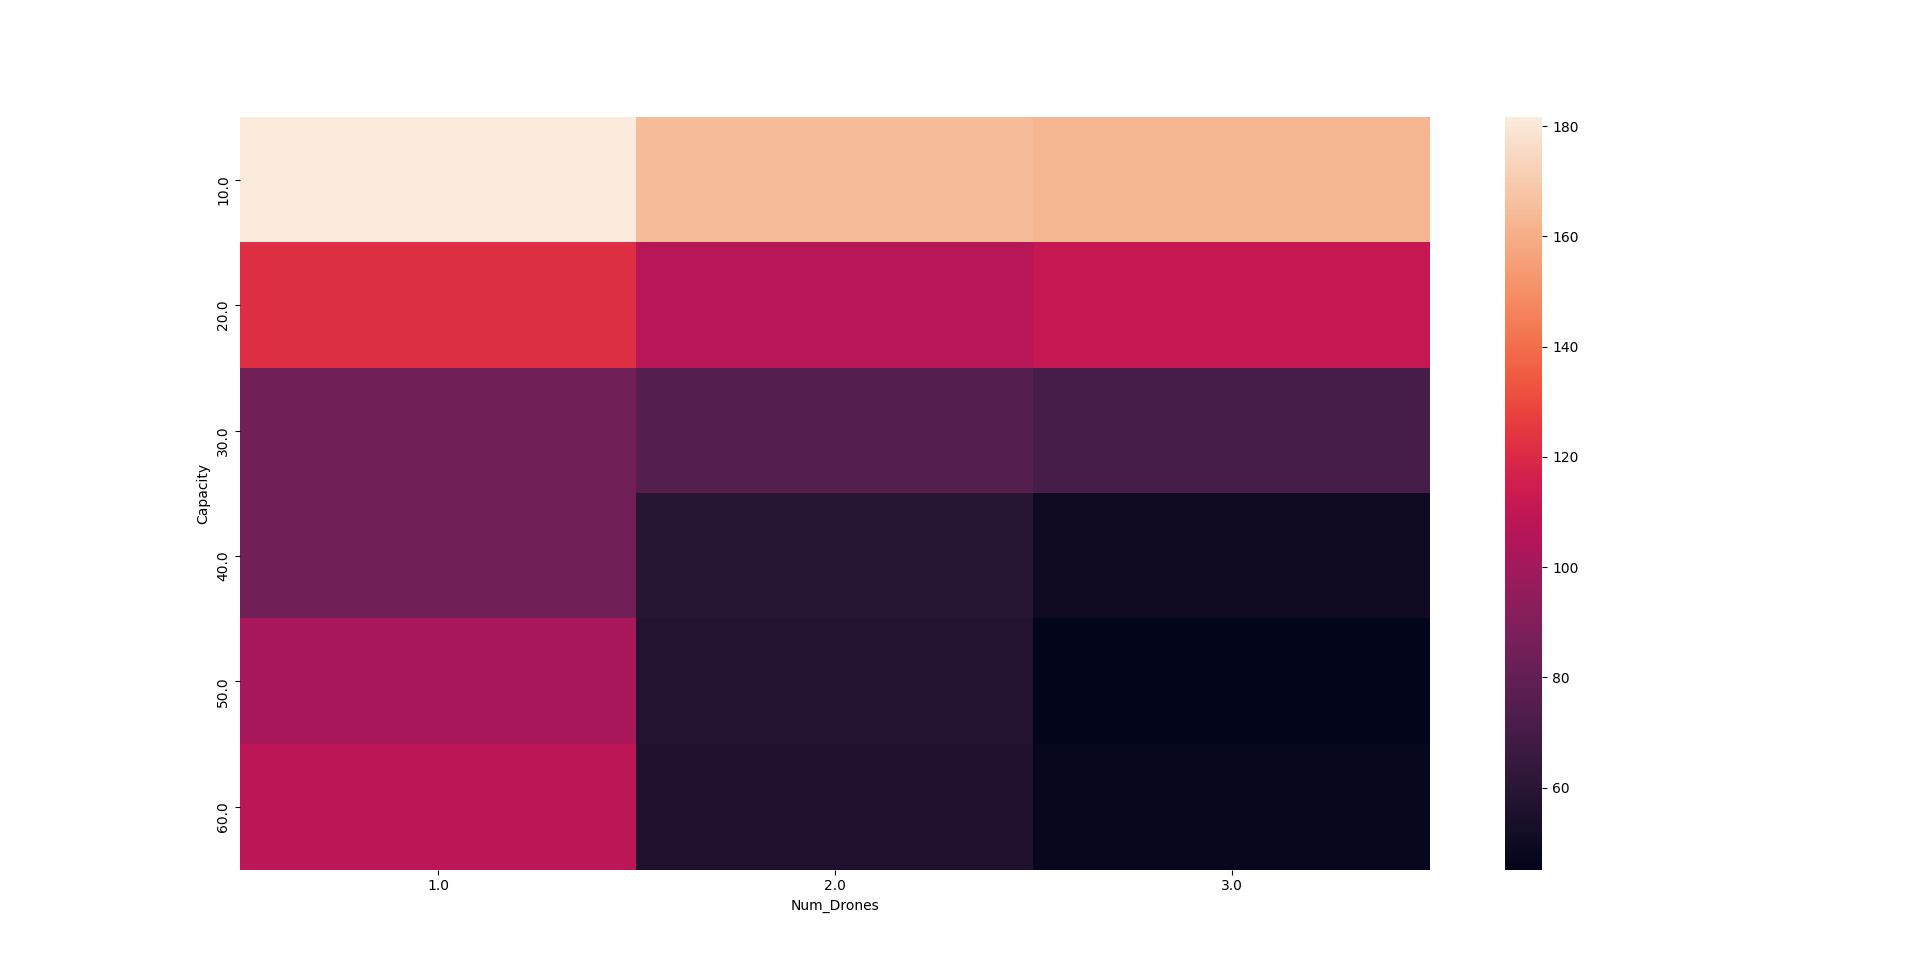
\includegraphics[width=\linewidth]{heatmap.png}
        \caption{Heatmap of objective function values depending on number of drones and drone capacities. The darker the color intensity the smaller the objective value. \label{fig:heatmap}}
        \end{figure}
	\end{frame}

    \begin{frame}{Case Study: Los Patios de C\'ordoba}
        Considering the current COVID-19 restrictions, we focus on the problem of preventing and identifying possible concentrations of people during events such as popular or religious festivals. In particular we consider the Courtyards Festival of Cordoba (\url{https://patios.cordoba.es/es/}).
        \begin{figure}[h!]
        \centering
        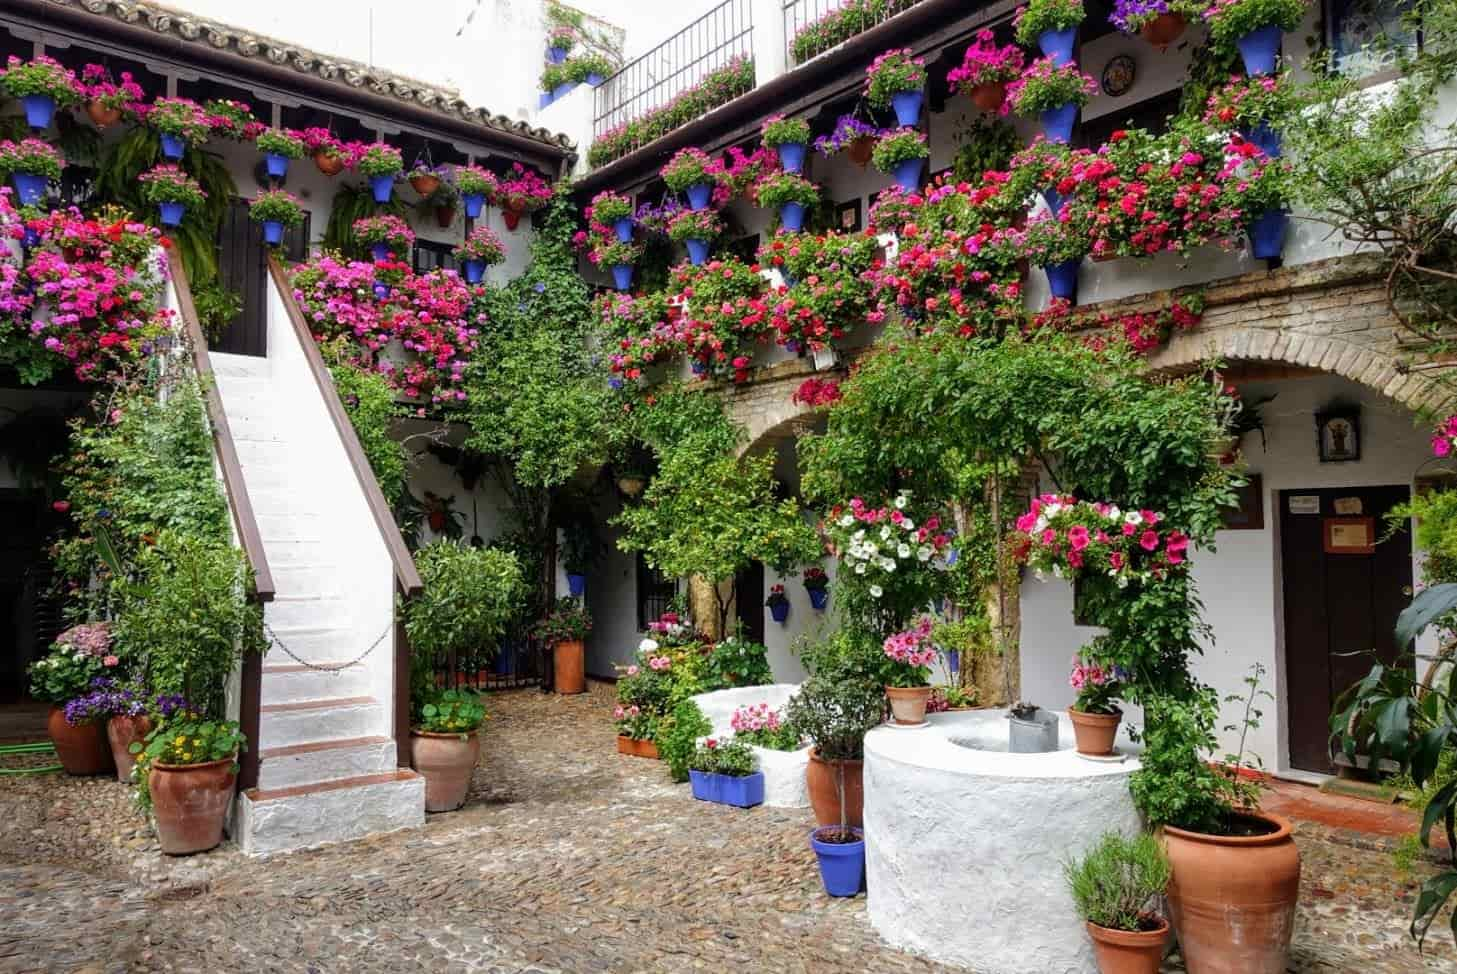
\includegraphics[width=0.33\linewidth]{patios_bonitos.jpg}
        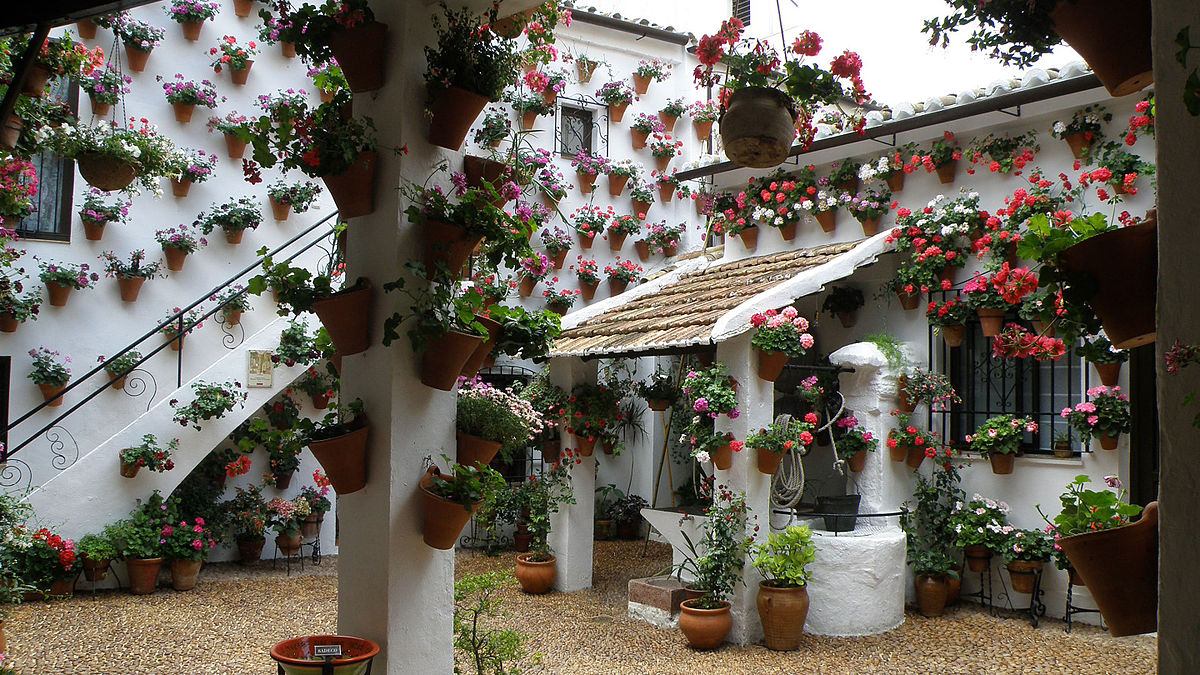
\includegraphics[width=0.4\linewidth]{patios_bonitos2.jpg}
        \end{figure}
    \end{frame}


    \begin{frame}{Case Study}
        \small
        We run the model on this scenario starting from the initial solution provided by the matheuristic, where the 6 coloured paths reported in the map of Figure \ref{fig:mapPF} represent the 6 target graphs to be visited, in this case inspected, by the fleet of drones. In addition, we suppose that the drones' speed is 100 km/h while that of the helicopter is  50 km/h aiming to minimize costs.
        \begin{figure}[h!]
        \centering
        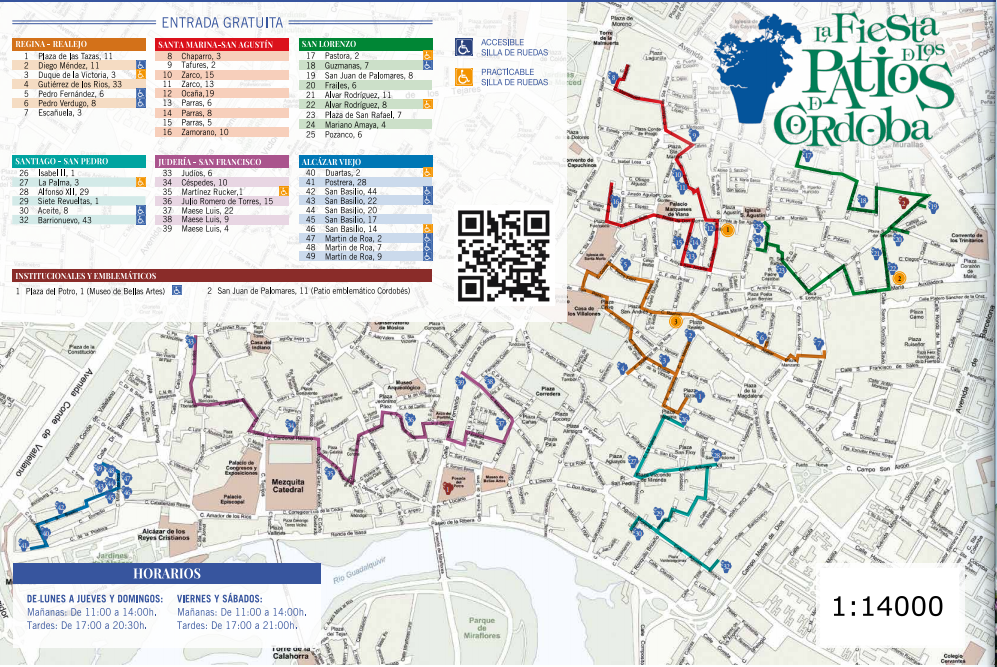
\includegraphics[width=0.5\linewidth]{first.png}
        \caption{Map of the Courtyards Festival in Cordoba. \label{fig:mapPF}}
        \end{figure}
    \end{frame}

    \begin{frame}{Case Study}
        We assume that the fleet is composed by three drones with an endurance equal to 2 hours, and we impose that each target graph must be fully visited (inspected) and the origin of the mothership tour coincides with the destination and it is located in an area of the city where it is possible to assume the take-off and landing of an helicopter.
        \begin{figure}[h!]
        \centering
        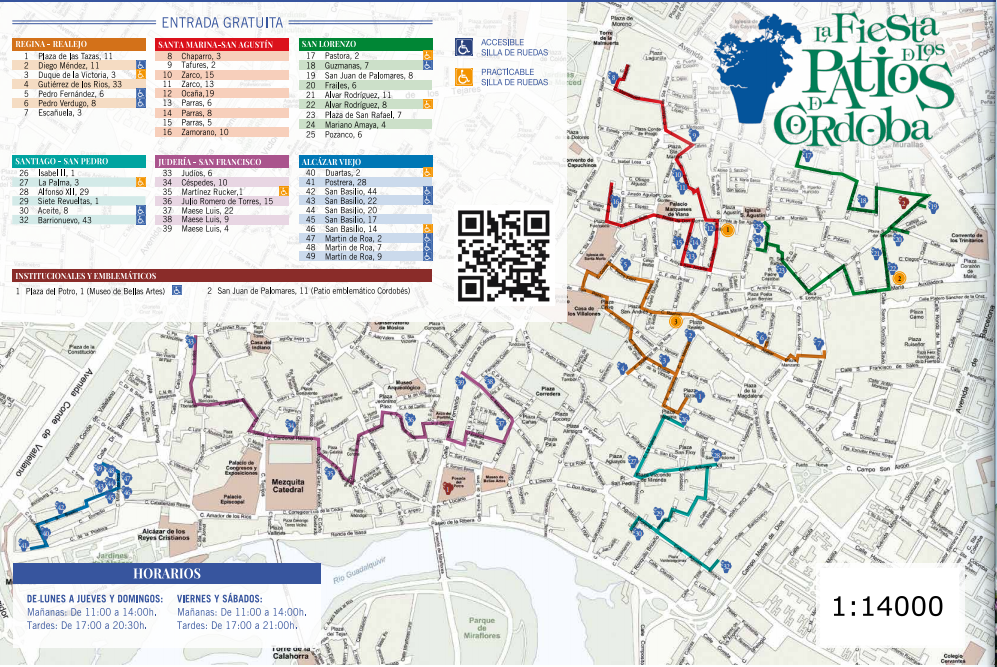
\includegraphics[width=0.5\linewidth]{first.png}
        \caption{Map of the Courtyards Festival in Cordoba. \label{fig:mapPF}}
        \end{figure}
    \end{frame}
    
    \begin{frame}{Case Study: Solution}
        \begin{figure}[h!]
        \centering
        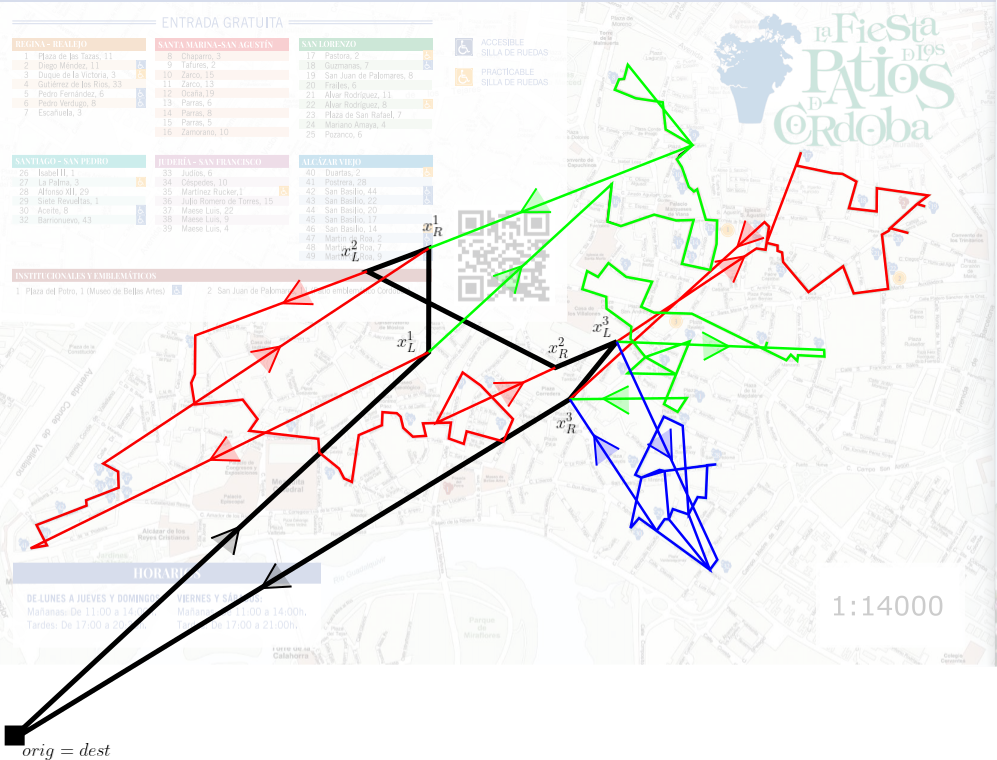
\includegraphics[width=0.7\linewidth]{third.png}
        \caption{The complete solution. \label{fig:tourD}}
        \end{figure}
    \end{frame}

    \begin{frame}{Acknowledgements}
        This research has been partially supported by Spanish Ministry of Education and Science/FEDER grant number  MTM2016-74983-C02-(01-02), and projects FEDER-US-1256951, Junta de Andaluc\'ia P18-FR-1422, CEI-3-FQM331 and  \textit{NetmeetData}: Ayudas Fundaci\'on BBVA a equipos de investigaci\'on cient\'ifica 2019.
    \end{frame}
    
	\begin{frame}
	    \bigskip
	    \begin{figure}
	        \centering
	        
\includegraphics[width=0.7\linewidth]{thank.jpg}
	    \end{figure}
	\end{frame}
	
	
	
	
	
	
	
	
	
	
	
	
	
	
	
	
	
	
	
	
	
\end{document}
